\documentclass[10pt,a4paper,final,oneside,openany]{memoir}

\usepackage[english]{babel}
\usepackage[utf8]{inputenc}
\usepackage[T1]{fontenc}
\usepackage[british]{isodate}

% Layout Fixes
\usepackage{booktabs} % nicer spacing between table rulers
\usepackage{microtype}
\usepackage{fixltx2e} % To prevent the figures from being placed
                      % out-of-order with respect to their
                      % "non-starred" counterparts


\usepackage{amsmath,amssymb, amsbsy}
\usepackage[amsmath,amsthm,thmmarks]{ntheorem}
\usepackage{graphicx}
\usepackage[export]{adjustbox}
\usepackage{float}
\usepackage{pdfpages}
\usepackage{color}
\usepackage{fancyvrb}
\usepackage{semantic}

\usepackage{enumitem} % Allows \begin{description}[style=nextline]

\usepackage{fixme}
\fxsetup{
    status=draft,
    author=,
    layout=margin,
    theme=color
}

\makeatletter
\newcommand*\idstyle{%
        \expandafter\id@style\the\lst@token\relax
}
\def\id@style#1#2\relax{%
        \ifcat#1\relax\else
                \ifnum`#1=\uccode`#1%
                        \color{blue}
                \fi
        \fi
}
\makeatother

% Bibliography
%\usepackage[style=alphabetic,natbib=true]{biblatex}
\usepackage[
hyperref=auto,
backend=biber,
style=numeric,
defernumbers=true
]{biblatex}

\usepackage[hyperindex,hidelinks]{hyperref}
\usepackage{cleveref}

% Fonts
\usepackage{palatino}
\linespread{1.05}
\usepackage[scaled]{beramono}

% customize chapter pages
\makepagestyle{myheadings}
\makepagestyle{myheadingschapterpage}
\makeevenfoot{myheadingschapterpage}{}{\thepage}{}
\makeoddfoot{myheadingschapterpage}{}{\thepage}{}
\aliaspagestyle{chapter}{myheadingschapterpage}
\aliaspagestyle{title}{myheadingschapterpage}
\makeevenhead{myheadings}{\hskip.5cm\leftmark}{}{}
\makeoddhead{myheadings}{}{}{\rightmark\hskip.5cm}
\makeevenfoot{myheadings}{}{\thepage}{}
\makeoddfoot{myheadings}{}{\thepage}{}
\pagestyle{myheadings}

\def\thefigure{\arabic{figure}}
\setcounter{tocdepth}{0}


\setsecnumdepth{subsection}
\setcounter{chapter}{0}
\setsecheadstyle{\large\bfseries\raggedright}
\setsubsecheadstyle{\bfseries}

% BIBLIOGRAPHY styling
% Print the DOI url out
%\newcommand*{\doi}[1]{DOI: \url{http://dx.doi.org/#1}}

\DeclareFieldFormat{doi}{\textsc{doi}: \url{http://dx.doi.org/#1}}
\DeclareNameAlias{default}{last-first/first-last}
%\DeclareFieldFormat{title}{\emph{#1}}
\renewcommand\mkbibnamefirst[1]{\textsc{#1}}
\renewcommand\mkbibnamelast[1]{\textsc{#1}}
\renewcommand*{\bibfont}{\footnotesize}

% No page numbers for parts in TOC
\cftpagenumbersoff{part}
% Footnote symbols
%\renewcommand*{\thefootnote}{\fnsymbol{footnote}}

% Figures
% \newsubfloat{figure}

\usepackage{sidecap}
\usepackage{caption}
\captionsetup{margin=0pt, font=small, labelfont=bf, format=hang}
% \setlength{\abovecaptionskip}{0pt}
% \setlength{\belowcaptionskip}{0pt}
\usepackage{subcaption}

% Default commands
\newcommand{\subimgwidth}{.48\textwidth}
\newcommand{\imgwidth}{.85\textwidth}


\newtheorem{example}{Example}
%
\theoremstyle{plain}
\theoremsymbol{\tiny $\Box$}
\newtheorem{definition}[equation]{Definition}


% Bitwise and and or operators
% http://tex.stackexchange.com/questions/39313/double-nested-logical-and-and-logical-or-symbols
\DeclareFontFamily{U}{matha}{\hyphenchar\font45}
\DeclareFontShape{U}{matha}{m}{n}{
      <5> <6> <7> <8> <9> <10> gen * matha
      <10.95> matha10 <12> <14.4> <17.28> <20.74> <24.88> matha12
      }{}

\newcommand{\bland}{\mathbin{
  \raisebox{.1ex}{%
    \rotatebox[origin=c]{-90}{\usefont{U}{matha}{m}{n}\symbol{\string"CE}}}}}
\newcommand{\blor}{\mathbin{
  \raisebox{.1ex}{%
    \rotatebox[origin=c]{90}{\usefont{U}{matha}{m}{n}\symbol{\string"CE}}}}}

% The colorcode environment lets us use colour markup inside verbatim blocks.
\DefineVerbatimEnvironment{colorcode}%
        {Verbatim}{fontsize=\small,commandchars=\\\{\}}

\DefineVerbatimEnvironment{bcolorcode}%
        {BVerbatim}{fontsize=\small,commandchars=\\\{\}}

% Visually Separate figures from text using a line.
\def\topfigrule{\vskip1ex\noindent\dotfill}
\def\botfigrule{\noindent\dotfill\vskip1ex}

%%% Local Variables: 
%%% mode: latex
%%% TeX-master: "thesis.tex"
%%% End: 


\usepackage[titelside, en, nat]{ku-forside}

\titel{Exploiting functional invariants}
\undertitel{to optimise parallelism: a dataflow approach}
\forfatter{Troels Henriksen -- \texttt{athas@sigkill.dk}}
\forfatterET{}
\forfatterTO{}
\opgave{Master's Thesis} % Findes kun under 'titelside'
\dato{February 2014}
\vejleder{Supervisors: Cosmin Eugen Oancea and Fritz Henglein}

\newcommand\boolt[0]{\texttt{bool}}
\newcommand\realt[0]{\texttt{real}}
\newcommand\chart[0]{\texttt{char}}
\newcommand\intt[0]{\texttt{int}}
\newcommand\aliases[1]{\textrm{aliases}(#1)}
\renewcommand\tilde[0]{{\raise.17ex\hbox{$\scriptstyle\sim$}}}
\newcommand{\LO}{$\mathcal{L}_0$}

\newcommand{\tagsc}[1]{\tag{\textsc{#1}}} % Fake Small Caps tagging
\newcommand{\nfrac}[2]{\frac{\displaystyle{#1}}{\displaystyle{#2}}}
\newcommand*{\bfrac}[2]{\genfrac{}{}{0pt}{}{#1}{#2}}

\definecolor{DikuRed}{RGB}{130,50,32}
\newcommand{\emp}[1]{\textcolor{DikuRed}{ #1}}
\definecolor{CosGreen}{RGB}{10,100,70}
\newcommand{\emphh}[1]{\textcolor{CosGreen}{ #1}}

\newcommand{\mymath}[1]{$ #1 $}
\newcommand{\myindx}[1]{_{#1}}
\newcommand{\myindu}[1]{^{#1}}
\newcommand{\mymathbb}[1]{\mathbb{#1}}
\newcommand{\cindx}[1]{\(\myindx{#1}\)}
\newcommand{\cindu}[1]{\(\myindu{#1}\)}

% Write "Part II" etc. in TOC instead of just "II"
\renewcommand*{\cftpartname}{Part\space}

\bibliography{bibliography}

\begin{document}
\frontmatter

 \clearpage

\maketitle
~
\vspace{3cm}
  \begin{abstract}
We present \LO{}, a purely functional programing language supporting nested
regular data parallelism and targeting massively parallel SIMD hardware
such as modern graphics processing units (GPUs).

\LO{} incorporates the following novel features:

\begin{itemize}
\item A type system for in-place modification and aliasing of arrays
  and array slices that ensures referential transparency, which in
  turn supports equational reasoning.

\item An assertion language for expressing bounds checks on
  dynamically allocated arrays, which can often be checked statically
  to eliminate dynamic bounds checks.

\item Compiler optimisations for hoisting bounds checks out of inner
  loops and performing loop fusion based on structural
  transformations.
\end{itemize}

We show that:

\begin{itemize}
\item The type system is simpler than existing linear and unique
  typing systems such Clean~\cite{barendsen1996uniqueness}, and more
  expressive than libraries such as DPH, Repa and
  Accelerate~\cite{Chak06DPH,keller2010regular,ArrayAccelerate}, for
  efficient array processing.

\item Our fusion transformation is capable of fusing loops whose
  output is used in multiple places, when possible without duplicating
  computation, a feature not found in other implementations of
  fusion~\cite{jones2001playing}.

\item The effectiveness of our optimisations is demonstrated on three
  real-world benchmark problems from quantitative finance, based on
  empirical run-time measurements and manual inspection of the
  optimised programs.  In particular, hoisting and fusion yield a
  sequential speed-up of up to 71\% compared to the unoptimised source
  code, even without any parallel execution.
\end{itemize}

The results suggest that the language design, expressiveness and
optimisation techniques of \LO{} can be realized across a range of
SIMD-architectures, notably existing GPUs and manycore-chips, to
simultaneously achieve portability and eventually performance
competitive with hand-coding.

The results reported are based on joint work with Cosmin Oancea, DIKU.

%%% Local Variables: 
%%% mode: latex
%%% TeX-master: "thesis.tex"
%%% End: 

  \end{abstract}

\setlength{\cftpartnumwidth}{4em}

% \clearpage
%  ~\thispagestyle{empty}
\clearpage
\tableofcontents*
%\openany
\phantomsection
\addcontentsline{toc}{chapter}{Preface}
\chapter*{Preface}
This dissertation is submitted in fulfillment of the graduate education
in computer science (\textit{Datalogi}) at the University of
Copenhagen, for Troels Henriksen.
%\openright
\mainmatter
\counterwithout{table}{chapter}
\counterwithout{figure}{chapter}
\chapter{Introduction}

For practically the entire lifetime of the electronic computer,
programmers have been used to an exponential growth in commonly
available computing power.  Until around 2006, this directly
manifested itself as improvements to sequential performance, although
physical limits made it uneconomical (or impossible) for this trend to
continue.  These days, hardware designers are making their machines
increasingly \textit{parallel}: rather than speeding up the individual
processors, as happened previously, \textit{more} processors, or more
\textit{specialised} processors, are added.  Thus, while computing
power is still growing, it has become increasingly necessary to write
programs that are parallel in order to take full advantage of modern
advancements in hardware.

One interesting development is the commoditisation of massively
parallel vector processors in the form of graphics cards.  While
hardware acceleration of graphics became commonplace in the 90s, it
was not until the rise of CUDA and OpenCL in 2006 that
\textit{General-Purpose computing on Graphics Processing Units}
(GPGPU) began to move into the mainstream.  Today, there are three
main ways to take advantage of this parallel processing power:

\begin{description}
\item[Low-level interfaces:] CUDA and OpenCL implementations are
  supplied by the GPU vendors.\footnote{Strictly. OpenCL has a broader
    focus, and seeks to provide an interface to heterogenous
    computation in general, but for the purpose of this thesis, we
    will consider OpenCL and CUDA to be GPU-oriented.}  These are very
  low-level, and provide a C-like programming interface.  Furthermore,
  GPU hardware has very complicated performance characteristics, and
  it can be hard to achieve optimal, or even good performance.
  Nevertheless, the full supported power of the devices is available
  at this level, and optimal performance is theoretically achievable,
  although in practice, specialist knowledge is required to achieve
  good results at this level.

  At the most basic level, all other approaches eventually boil down
  to talking to a low-level interface.

\item[Libraries:] Some programming libraries aimed at high-peformance
  computing have been rewritten to take advantage of GPU acceleration.
  For example, Nvidia provides CUBLAS~\cite{nvidia2008cublas}, an
  implementation of the well-known BLAS array operations API.  These
  libraries are typically written by experts, and come close to peak
  potential performance on the target hardware.  It is generally easy
  to use these libraries from any language offering a good foreign
  function interface, and it is thus an efficient way to reach a large
  number of potential users.  Usage of these libraries requires little
  in the way of GPU knowledge, or indeed knowledge about parallel
  programming at all.

  On the downside, although each discrete function may be
  well-optimised in isolation, the library approach does not permit
  optimisation of composed operations.  For example, if a library
  exports a function \texttt{mult} to multiply two matrices, and we
  use it in two invocations to multiply three matrices, as in
  \texttt{mult(x,mult(y,z))}, the library will likely not be as fast
  as if we used a specialised ternary multiplication function.
  Although particularly clever libraries may use a variant of lazy
  evaluation to delay computation and optimise some composed
  operations~\cite{kristensenbohrium}, the optimisation potential is
  still limited as long as the program cannot be inspected directly.

  The library approach is very popular in practice, with many
  high-performance computing libraries now possessing GPGPU backends.

\item[Data-parallel programming languages:] The final way to perform
  GPGPU is to integrate GPU support directly into a programming
  language, with full compiler support.  This permits code generation
  based on a global view of the entire computation, at least in
  theory, and optimise with full knowledge of the program.  There
  appears to be two main paths within the programming language
  approach:

\begin{description}
\item[Embedded languages:] Somewhat similar to the library approach,
  this integrates GPGPU support in an existing language as an
  \textit{Embedded Domain Specific Language}
  (EDSL)~\cite{czarnecki2004dsl}.  The distinction between an EDSL and
  a library is often fuzzy, with the distinction typically being about
  the level of composability offered, and whether the EDSL follows the
  same evaluation rules as the host language.  Further blurring the
  issue, some EDSLs use syntactical extensions -- for example through
  macros~\cite{kohlbecker1986hygienic} or
  quasiquotation~\cite{mainland2007s} -- while others take advantage
  of the host languages existing syntactical facilities.

  The limitations for EDSLs are similar to the ones for libraries.
  For example, the embedded language must be expressible in the type
  system of the host language.  It also varies how much support the
  host language provides for hooking into the compiler, in order to
  perform optimisation.  On the other hand, much of the infrastructure
  of the host language will be inherited by the EDSL, leading to a
  much simpler implementation, compared to writing a full compiler.
  Furthermore, due to the integration with the host language, EDSL
  usage can be very seamless.  On the other hand, it is extremely hard
  to access an EDSL from outside of the host language.

  DPH, Repa and
  Accelerate~\cite{Chak06DPH,keller2010regular,ArrayAccelerate} are
  examples of data-parallel EDSLs for Haskell, with Accelerate suppors
  OpenCL and CUDA backends.

\item[Independent languages:] The final approach is to write an entire
  compiler targeting GPGPU execution.  This provides total control, at
  the cost of greatly increased implementation complexity.
  Furthermore, it can be difficult to integrate components written in
  a these new languages into existing code-bases written in mainstream
  languages.  Nevertheless, the language can be designed from the
  bottom up for efficient parallel execution, without compromises due
  to host language integration.  The NESL~\cite{BlellochCACM96NESL}
  language is an early ('96) example of a programming language
  designed entirely for data-parallel execution.  Although designed
  before the proliferation of GPUs, a GPU backend has recently been
  developed~\cite{bergstrom2012nested}.  Another example of such a
  language is Single-Assignment C (SAC)~\cite{grelck2006sac}.

  In a way, we could also consider the OpenCL and CUDA kernel
  languages themselves to be in this category, but we only consider
  high-level languages to be proper members of this group.
\end{description}
\end{description}

The library approach is effective if a library exists for the specific
problem the programmer is attempting to solve, but will often be
neither sufficiently fast nor expressive for new domains.  EDSL suffer
from a similar problem -- in particular, nested parallelism is
generally very poorly supported.  The NESL and SAC languages are more
expressive, but their implementation does not perform many advanced
optimisations.

In this thesis, we will present \LO{}, an independent language
designed for parallel execution.  We have chosen to implement \LO{} as
a non-embedded language in order to have more design freedom, as we do
not need to, e.g., fit \LO{} into the type system of an existing
language.

Loop fusion is one of the most important code transformations, as it
has the potential for substantially optimising both memory hierarchy
overhead and, sometimes asymptotically, space requirement.  In
functional languages, fusion is naturally and relatively easily
derived from the producer-consumer relation between program constructs
that expose a rich, higher-order algebra of program invariants, such
as the \texttt{map-reduce} list homomorphisms.

In imperative languages, fusing producer-consumer loops requires
dependency analysis on arrays applied at loop-nest level.  Such
analysis, however, has often been labeled as ``heroic effort'' and, if
at all, is supported only in its simplest and most conservative form
in industrial compilers.

... \fixme{Insert more - convince reader that my work addresses an
  important problem, and that I will give a well thought-out solution.
  Why is \LO{} functional, and why does it support sequential loops
  anyway?}

Throughout this thesis, we will often refer to a vaguely defined
``programmer'', as well as ascribe various motives and expectations to
this nebulous being.  While \LO{} is intended as an intermediate
language, and in the end is intended as a target language by compilers
for higher-level languages, it has a well-defined human-readable (and
writable) syntax, and can be programmed directly.  Indeed, all extant
\LO{} programs have been written by hand.  Thus, when ``the
programmer'' is referenced, we can refer to either an actual human, or
a compiler generating \LO{} code.  For our purposes, these will have
identical motives, although a human programmer may complain somewhat
more vocally about the lack of syntactical niceties in the language.

\section{Contributions}

We present a purely functional data-parallel programming language,
\LO{}, with support for nested parallelism.  The language supports a
method \fixme{Why do I support nested parallelism?  Why only regular
  arrays?  Why are in-place updates supported (cross-iteration
  dependent loops)} for safely performing in-place updates of array
data through a type system concept called \textit{uniqueness types}.
Through the translation of real-world financial programs to \LO{}, we
demonstrate the practical usefulness of this language feature.

We describe the design and implementation of several optimisations,
notably hoisting bounds checks out of inner loops, and loop fusion
based on a structural transformation.  The fusion transformation is
capable of fusing loops whose output is used in multiple places, when
possible without duplicating computation.\fixme{Why is it important to
  hoist bounds checks?  Because we target aggressive (static+dynamic)
  analysis; this is an instance of optimising arbitrary predicates.}

The benefits of our optimisations are demonstrated on three real-world
financial benchmarks.  It is shown that the compiler is able to hoist
bounds checks and other assertions outside of loops.

The effectiveness of fusion is demonstrated via compiler
instrumentation and quantitative and qualitative measurements on the
three benchmarks, in the form of inspecting the changes in program
dataflow.  This shows that always refusing to duplicate computation is
too conservative on parallel hardware, and discuss potential
directions for further improvement.

The implementation of the \LO{} compiler consists of roughly ten
thousand lines of Haskell (ignoring comments and blank lines), and it
is hosted and publicly browsable at
\url{https://github.com/HIPERFIT/L0Language}.

Parts of this thesis, in particular the core of the fusion algorithm
in \cref{chap:fusion}, has been previously published as

\begin{quote}
\fullcite{Henriksen:2013:TGA:2502323.2502328}
\end{quote}

\section{Report outline}

The remainder of the report is structured as follows.
\Cref{chap:l0language,chap:uniqueness-types} will introduce the
programmer-visible part of \LO{} and serves as a language reference.
\Cref{chap:internal} presents a slight modification of the external
language, that makes it more amenable to transformation and
optimisation.  \Cref{chap:first-order-optimisations} discusses various
classical optimisations in the context of \LO{}.  \Cref{chap:fusion}
covers \textit{loop fusion}, an important optimisation, while
\cref{chap:fusion-enabling-soac-transformations,chap:hindrance-removal}
cover transformations that enable other optimisations (although
particularly fusion).

\section{Notation}

In various places, I will use an \(\overline{\text{overline}}\) to
indicate a comma-separated sequence of terms.  For example, when
describing a function call, rather than writing:
\[
f(e_{1},\ldots,e_{n})
\]
I may instead write:
\[
f(\overline{es})
\]
I may also use this in conjunction with expliclt arguments, as in:
\[
f(e_{start},\overline{es},e_{end})
\]

%%% Local Variables:
%%% mode: latex
%%% TeX-master: "thesis"
%%% End:


\nocite{uffe}

\part{Language Design}
\label{part:languagedesign}

\chapter{The \LO{} language}
\label{chap:l0language}

\LO{} is a purely functional, call-by-value, mostly first-order
language that permits bulk operations on arrays using
\textit{second-order array combinatrs} (SOACs).
\Cref{sec:fo-l0,sec:soacs} will present \LO{} through informal
walkthrough of the major language concepts, whilst a complete
reference of language constructs is given in \cref{sec:l0-reference}.

\section{First-order \LO{}}
\label{sec:fo-l0}

\begin{figure}[bt]
\begin{tabular}{lrll}
$t$ & $::=$ & \texttt{int} & (Integers) \\
& $|$ & \texttt{real} & (Floats) \\
& $|$ & \texttt{bool} & (Booleans) \\
& $|$ & \texttt{char} & (Characters) \\
& $|$ & \texttt{\{$t_{1}$, \ldots, $t_{n}$\}} & (Tuples) \\
& $|$ & \texttt{[$t$]} & (Arrays) \\
& $|$ & \texttt{*[$t$]} & (Unique arrays) \\
\\
$k$ & $::=$ & $n$ & (Integer)\\
& $|$ & $x$ & (Decimal number) \\
& $|$ & $b$ & (Boolean)\\
& $|$ & $c$ & (Character)\\
& $|$ & \texttt{\{$v_{1},\ldots,v_{n}$\}} & (Tuple) \\
& $|$ & \texttt{[$v_{1},\ldots,v_{n}$]} & (Array) \\
\\
$p$ & $::=$ & \texttt{\textbf{id}} & (Name pattern)\\
& $|$ & \texttt{($p_{1}$, \ldots, $p_{n}$)} & (Tuple pattern) \\
\end{tabular}
\caption{\LO{} syntax}
\label{fig:fo-syntax}
\end{figure}

\begin{figure}[bt]
\begin{tabular}{lrll}
$e$ & $::=$ & $k$ & (Constant)\\
& $|$ & $v$ & (Variable)\\
& $|$ & \texttt{($e_{1}$,\ldots,$e_{n}$)} & (Tuple expression) \\
& $|$ & \texttt{\{$e_{1}$,\ldots,$e_{n}$\}} & (Array expression) \\
& $|$ & $e_{1} \odot{} e_{2}$ & (Binary operator) \\
& $|$ & \texttt{-$e$} & (Prefix minus) \\
& $|$ & \texttt{not $e$} & (Logical negation) \\
& $|$ & \texttt{if $e_{1}$ then $e_{2}$ else $e_{3}$} & (Branching) \\
& $|$ & \texttt{$v$[$e_{1}$, \ldots, $e_{n}$]} & (Indexing) \\
& $|$ & \texttt{$v$($e_{1}$, \ldots, $e_{n}$)} & (Function call) \\
& $|$ & \texttt{let $p$ = $e_{1}$ in $e_{2}$} & (Pattern binding) \\
& $|$ & \texttt{zip($e_{1}$, \ldots, $e_{n}$)} & (Zipping) \\
& $|$ & \texttt{unzip($e$)} & (Unzipping) \\
& $|$ & \texttt{iota($e$)} & (Range) \\
& $|$ & \texttt{replicate($e_{n}$, $e_{v}$)} & (Replication) \\
& $|$ & \texttt{size($e$)} & (Array length) \\
& $|$ & \texttt{reshape(($e_{1}$,\ldots,$e_{n}$), $e$)} & (Array reshape) \\
& $|$ & \texttt{transpose($e$)} & (Transposition) \\
& $|$ & \texttt{split($e_{1}$, $e_{2}$)} & (Split $e_{2}$ at index $e_{1}$) \\
& $|$ & \texttt{concat($e_{1}$, $e_{2}$)} & (Concatenation) \\
& $|$ & \texttt{let $v_{1}$ = $v_{2}$ with} & (In-place update) \\
&     & \texttt{\ \ [$e_{1}$,\ldots,$e_{n}$] <- $e_{v}$} \\
&     & \texttt{in $e_{b}$} \\
& $|$ & \texttt{loop ($p$ = $e_{1}$) =} & (Loop) \\
&     & \texttt{\ \ for $v$ < $e_{2}$ do $e_{3}$} \\
&     & \texttt{in $e_{4}$} \\
\end{tabular}
\\
\begin{tabular}{lrll}
$fun$ & $::=$ & \texttt{fun $t$ $v$($t_{1}$ $v_{1}$,\ldots $t_{n}$ $v_{n}$) = $e$} \\
\\
$prog$ & $::=$ & $\epsilon$ \\
       & $|$   & $fun$ $prog$
\end{tabular}
\caption{\LO{} syntax, continued}
\label{fig:fo-syntax-continued}
\end{figure}

The syntax of \LO{}, as seen on \cref{fig:fo-syntax} and
\cref{fig:fo-syntax-continued}, is heavily inspired by Haskell and
Standard ML.  An identifier stats with a letter, followed by any
number of letters, digits and underscores.  Numeric, string and
character literals use the same notation as Haskell (which is very
similar to C), including all escape characters.  Comments are
indicated with \texttt{//} and span to end of line.

An \LO{} program consists of a sequence of \emph{function
  definitions}, of the following form.

\begin{colorcode}
  fun \textit{return-type} \textit{name}(\textit{params...}) = \textit{body}
\end{colorcode}

A function must declare both its return type and the types of all
parameters.  All functions (except for inline anonymous functions; see
below) are defined globally.  \LO{} does not use type inference.
Symbolic constants are not supported, although 0-ary functions can be
defined.  As a concrete example, here is the recursive definition of
the factorial function in \LO{}.
\begin{colorcode}
  fun int fact(int n) =
    if n = 0 then 1
             else n * fact(n-1)
\end{colorcode}
Indentation has no syntactical significance in \LO{}, but recommended for
readability.

The syntax for tuple types is a comma-separated list of types or
values enclosed in braces, so \texttt{\{int, real\}} is a pair of an
integer and a floating-point number.  Both single-element and empty
tuples are permitted.  Array types are written as the element type
surrounded by brackets, meaning that \texttt{[int]} is a
one-dimensional array of integers, and \texttt{[[[\{int, real\}]]]} is a
three-dimensional array of tuples of integers and floats.  An
immediate array is written as a sequence of elements enclosed by
brackets.
\begin{colorcode}
  [1, 2, 3]       // Array of type [int].
  [[1], [2], [3]] // Array of type [[int]].
\end{colorcode}
All arrays must be \emph{regular} (often termed \emph{full}) - for
example, all rows of a two-dimensional array must have the same number
of elements.
\begin{colorcode}
  [[1, 2], [3]]      // Compile-time error.
  [iota(1), iota(2)] // Run-time error.
\end{colorcode}
Arrays are indexed using the common row-major notation, e.g.,
\texttt{a[i1, i2, i3...]}.  An indexing is said to be \textit{full} if
the number of given indexes is equal to the dimensionality of the
array.

A \texttt{let}-expression can be used to refer to the result of a
subexpression:
\begin{colorcode}
  let z = x + y in ...
\end{colorcode}
Recall that \LO{} is eagerly evaluated, so the right-hand side of the
\texttt{let} is evaluated exactly once, at the time it is first
encountered.

Two-way \texttt{if-then-else} is the only branching construct in \LO{}.
Pattern matching is supported in a limited way for taking apart
tuples, but this can only be done in \texttt{let}-bindings, and not
directly in a function argument list.  Specifically, the following
function definition is not valid.
\begin{colorcode}
  fun int sumpair(\{int, int\} \{x, y\}) = x + y // WRONG!
\end{colorcode}
Instead, we must use a let-binding explicitly, as follows.
\begin{colorcode}
  fun int sumpair(\{int, int\} t) =
    let \{x,y\} = t in x + y
\end{colorcode}
Pattern-matching in a binding is the only way to access the components
of a tuple.

Function calls are written as the function name followed by the
arguments enclosed in parentheses.  All function calls must be fully
saturated - currying is only permitted in SOACs (see
\cref{sec:soacs}).

\subsection{Sequential loops}

\LO{} has a built-in syntax for expressing certain tail-recursive
functions.  Consider the following tail-recursive formulation of a
function for computing the Fibonacci numbers.
\begin{colorcode}
  fun int fib(int n) = fibhelper(1,1,n)

  fun int fibhelper(int x, int y, int n) =
    if n = 1 then x else fibhelper(y, x+y, n-1)
\end{colorcode}
We can rewrite this using the \texttt{loop} construct.
\begin{colorcode}
  fun int fib(int n) =
    loop (\{x, y\} = \{1,1\}) = for i < n do
                              {y, x+y}
    in x
\end{colorcode}
The semantics of this is precisely as in the tail-recursive function
formulation.  In general, a loop
\begin{colorcode}
  loop (\emph{pat} = \emph{initial}) = for \emph{i} < \emph{bound} do \emph{loopbody}
  in \emph{body}
\end{colorcode}
has the following semantics:

\begin{enumerate}
  \item Bind \textit{pat} to the initial values given in \textit{initial}.
  \item While $\textit{i} < \textit{bound}$, evaluate
    \textit{loopbody}, rebinding \textit{pat} to be the value returned
    by the body.  At the end of each iteration, increment \textit{i}
    by one.
  \item Evaluate \textit{body} with \textit{pat} bound to its final
    value.
\end{enumerate}
The purpose of \texttt{loop} is partly to render some sequential
computations slightly more convenient, partly to express certain loop
optimisations in the compiler.  Semantically, it is completely
equivalent to the call to its corresponding tail-recursive function.
For example, denoting by \texttt{t} the type of \texttt{x}, the loop
in \cref{fig:loop-recursion} has the semantics of a call to the
tail-recursive function on the right-hand side.

\begin{figure}
\begin{minipage}{0.35\columnwidth}
\begin{colorcode}
loop (x = a) =
  for i < n do
    g(x)
in body
\end{colorcode}
\end{minipage}
\begin{minipage}{0.05\columnwidth}
$\Rightarrow$
\end{minipage}
\begin{minipage}{0.6\columnwidth}
\begin{colorcode}
fun t f(int i, int n, t x) =
  if i >= n then x
     else f(i+1, n, g(x))

let x = f(i, n, a)
in body
\end{colorcode}
\end{minipage}
\caption{Loop to recursive function}
\label{fig:loop-recursion}
\end{figure}

\subsection{In-place updates}

General modification of array elements is done using the
\texttt{let-with} construct.  In its most general form, it looks as
follows.
\begin{colorcode}
  let \textit{dest} = \textit{src} with [\textit{indexes}] <- \textit{value}
  in \textit{body}
\end{colorcode}
This evaluates \textit{body} with \textit{dest} bound to the value of
\textit{src}, except that the element(s) at the position given by
\textit{indexes} take on the new value \textit{value}.\footnote{Yes,
  this is the \emph{third} binding construct in the language, ignoring
  function abstraction!}  The given indexes need not be complete, but
in that case, \textit{value} must be an array of the proper size.  As
an example, here's how we could replace the third row of an $n\times3$
array.
\begin{colorcode}
  let b = a with [2] <- [1,2,3] in b
\end{colorcode}
Whenever $\textit{dest} = \textit{src}$, we can write
\begin{colorcode}
  let \textit{dest}[\textit{indexes}] = \textit{value} in \textit{body}
\end{colorcode}
as a shortcut.  Note that this has no special semantic meaning, but is
simply a case of normal name shadowing.  Let-with has some unusual
restrictions to permit in-place modification of the \textit{src}
array, as described in \cref{chap:uniqueness-types}.

For example, the loop given below implements the ``imperative''
version of matrix multiplication of two $M\times M$ matrices.

\begin{colorcode}
fun *[[int]] matmultImp(int N, [[int]] a, [[int]] b) =
    let res = replicate(N, iota(N)) in
    loop (res) = for i < N do
        loop (res) = for j < N do
            let partsum =
                let res = 0 in
                loop (res) = for k < N do
                    let res = res + a[i,k] * b[k,j]
                    in  res
                in res
            in let res[i,j] = partsum in res
        in res
    in res
\end{colorcode}

\section{SOACs}
\label{sec:soacs}

The language presented in the previous section is in some sense
``sufficient'', in that it is Turing-complete, and can express
imperative-style loops in a natural way with \texttt{do}-loops.
However, \LO{} is not intended to be used in such a way - bulk
operations on arrays should be expressed via the four
\textit{second-order array combinators} (SOACs) shown in
\cref{fig:soacs}, as the optimisations covered in later chapters are
expressed as transformations on these.

\begin{figure}[bt]
\begin{tabular}{lrll}
$l$ & $::=$ & \texttt{fn $t$ ($t_{1}$ $v_{1}$, \ldots, $t_{n}$ $v_{n}$) => $e$} & (Anonymous function) \\
& $|$ & \texttt{\textbf{id} ($e_{1}$, \ldots, $e_{n}$)} & (Curried function) \\
& $|$ & \texttt{op $\odot$ ($e_{1}$, \ldots, $e_{n}$)} & (Curried operator) \\
\\
$e$ & $::=$ & \texttt{map($l$, $e$)} \\
    & $|$ & \texttt{filter($l$, $e$)} \\
    & $|$ & \texttt{reduce($l$, $x$, $e$)} \\
    & $|$ & \texttt{scan($l$, $x$, $e$)} \\
    & $|$ & \texttt{redomap($l_{r}$, $l_{m}$, $x$, $e$)} \\
\end{tabular}
\caption{Second-order array combinators}
\label{fig:soacs}
\end{figure}

The semantics of the \textsc{soac}s is identical to the similarly-named
higher-order functions found in many functional languages, but we
reproduce it here for completeness.  The types given are not \LO{}
types, but a Haskell-inspired notation, since the \textsc{soac}s cannot
be typed in \LO{} itself.
\begin{align*}
\texttt{map($f$,$a$)}
& :: (\alpha\rightarrow\beta)\rightarrow[\alpha]\rightarrow[\beta] \\
& \equiv \texttt{\{$f$($a$[0]), \ldots, $f$($a$[n])\}}
\end{align*}
\begin{align*}
\texttt{ filter}
& :: (\alpha\rightarrow\texttt{bool})\rightarrow[\alpha]\rightarrow[\alpha] \\
\texttt{ filter($f$,a)} & \equiv \texttt{\{$a$[i] | $f$($a$[i]) = \texttt{True }\}}
\end{align*}
\begin{align*}
\texttt{ reduce}
& :: (\alpha\rightarrow\alpha\rightarrow\alpha)\rightarrow\alpha\rightarrow[\alpha]\rightarrow\alpha \\
\texttt{ reduce($f$,$x$,$a$)} & \equiv \texttt{ $f$(\ldots($f$($f$($x$,$a$[0]), $a$[1])\ldots), $a$[n])}
\end{align*}
\begin{align*}
\texttt{ scan}
& :: (\alpha\rightarrow\alpha\rightarrow\alpha)\rightarrow\alpha\rightarrow[\alpha]\rightarrow[\alpha] \\
\texttt{ scan($f$,$x$,a)} & \equiv \texttt{\{$f$($x$,$a$[0]), $f$($f$($x$,$a$[0]),$v$[1]),\ldots\}}
\end{align*}

In particular, note that \texttt{scan} and \texttt{reduce} require
binary associative operators and \texttt{scan} is an inclusive prefix
scan.  The value given as the initial value of the accumulator must be
the neutral element for the function.  These properties are not
checked by the \LO{} compiler, and are the responsibility of the
programmer.

\texttt{redomap} is a special case -- it is not intended for use by
the programmer, but used internally for fusing \texttt{reduce} and
\texttt{map}.  Its semantics is as follows.
\begin{align*}
\texttt{redomap}
& :: (\alpha\rightarrow\alpha\rightarrow\alpha)\rightarrow(\alpha\rightarrow\beta\rightarrow\alpha)\\
& \quad\rightarrow\alpha\rightarrow[\beta]\rightarrow\alpha \\
\texttt{redomap($\odot$,$g$,$x$,$v$)} & \equiv \texttt{foldl($g$, $x$, $v$)}
\end{align*}
Note that the runtime semantics is a left-fold, not a normal \LO{}
\texttt{reduce}.  In particular, $g$ need not be associative.  We use
a Haskell-like syntax to explain the
rationale behind \texttt{redomap}:\\
$(\texttt{reduce}\ \odot\ e)\ \circ\ (\texttt{map}\ f)$ can be
formally transformed, via the list homomorphism (\textsc{lh})
promotion lemma~\cite{BirdListTh}, to an
equivalent form:  \\
$(\texttt{reduce}\ \odot\ e)\ \circ\ (\texttt{map}\ f)\
\emphh{\equiv}\ \texttt{reduce}\ \odot\
e\ \circ\ \texttt{map}\ (\emp{\texttt{reduce}\ \odot\ e\ \circ\ \texttt{map}\ f})\ \circ\ \texttt{split}_{p}$\\
where the original list is distributed to $p$ parallel processors,
each of which execute the original map-reduce computation sequentially
and, at the end, reduce in parallel the per-processor result using the
operator $\odot$.  Hence, the \textit{inner} map-reduce can be
rewritten as a left-fold:\\
$(\texttt{reduce}\ \odot\ e)\ \circ\ (\texttt{map}\ f)\
\emphh{\equiv}\ \texttt{reduce}\ \odot\
e\ \circ \texttt{map} \ (\emp{\texttt{foldl}\ g\ e})\ \circ\ \texttt{split}_{p}$\\
Where $g$ is a function generated from the composition of $f$ and
$\circ$.  It follows that in order to generate parallel code for \\
\texttt{(reduce $\odot$ $e$) $\circ$ (map $f$)} it is sufficient to
record either $\odot$ and $f$, or $\odot$ and $g$. We choose the
latter, i.e., \texttt{redomap($\odot$, $g$, $e$)}, because it allows a
richer compositional algebra for fusion.  In particular, it allows us
to fuse \texttt{reduce~$\circ$~map~$\circ$~filter} into a
\texttt{redomap} without duplicating computation, as described in
\cref{chap:fusion}.

\section{Language reference}
\label{sec:l0-reference}

The builtin types in \LO{} are \intt{}, \realt{}, \boolt{} and \chart{}, as
well as their combination in tuples and arrays.

The following list describes every syntactical language construct in
the language.

\begin{description}
  \item[\textit{constant}]\hfill\\
    Evaluates to itself.

  \item[\textit{var}]\hfill\\
    Evaluates to its value in the environment.

  \item[\texttt{\textit{x} \textbf{arithop} \textit{y}}] \hfill\\
    Evaluate the binary operator on its operands, which must both be
    of either type \intt{} or \realt.  The following operators are
    supported: \texttt{+}, \texttt{*}, \texttt{-}, \texttt{/},
    \texttt{\%}, \texttt{=}, \texttt{<}, \texttt{<=}, \texttt{pow}.

  \item[\texttt{\textit{x} \textbf{bitop} \textit{y}}] \hfill\\
    Evaluate the binary operator on its operands, which must both be
    of type \intt.  The following operators are supported:
    \texttt{\^}, \texttt{\&}, \texttt{|}, \texttt{>>}, \texttt{<<},
    i.e., bitwise xor, and, or, and arithmetic shift right and left.

  \item[\texttt{\textit{x} \&\& \textit{y}}]\hfill\\
    Short-circuiting conjunction, both operands must be of type \boolt.

  \item[\texttt{\textit{x} || \textit{y}}]\hfill\\
    Short-circuiting disjunction, both operands must be of type \boolt.

  \item[\texttt{not \textit{x}}]\hfill\\
    Logical negation of \textit{x}, which must be of type \boolt.

  \item[\texttt{-\textit{x}}]\hfill\\
    Numerical negation of \textit{x}, which must be of type \realt{} or \intt.

  \item[\texttt{a[i]}]\hfill\\
    Return the element at the given position in the array.  The index
    may be a comma-separated list of indexes.

  \item[\texttt{zip($a_1, \ldots, a_n$)}]\hfill\\
    Zips together the elements of the outer dimensions of arrays $a_1,
    \ldots, a_n$.  Static or runtime check is required to check that
    the sizes of the outermost dimension of arrays $a_1, \ldots, a_n$
    are the same.  If this invariant does not hold, program execution
    stops with an error.
  \item[\texttt{unzip($a$)}]\hfill\\
    If the type of $a$ is $[\{t_1, \ldots, t_n\}]$ then the result is
    a tuple of $n$ arrays, i.e., $\{[t_1], \ldots, [t_n]\}$, otherwise
    error.

  \item[\texttt{iota(\textit{n})}]\hfill\\
    An array of the integers from $0$ to \textit{n}.

  \item[\texttt{replicate(\textit{n}, \textit{a})}]\hfill\\
    An array consisting of \textit{n} copies of \textit{a}.

  \item[\texttt{size($k$, \textit{a})}]\hfill\\
    The size of dimension $k$ of array \textit{a}.  $k$ must be a
    static integral constant.

  \item[\texttt{split(\textit{n}, \textit{a})}]\hfill\\
    Partitions the given array into two disjoint arrays
    \texttt{\textit{a}[$0\ldots{}n$]},
    \texttt{\textit{a}[$n+1\ldots{}$]}, returned as a tuple.

  \item[\texttt{concat(\textit{a}, \textit{b})}]\hfill\\
    Concatenate the rows/elements of one array with another.  The
    shape of the two arrays must be identical in all but the first
    dimensionel.

  \item[\texttt{copy(\textit{x})}]\hfill\\
    Return a deep copy of the argument.  Semantically, this is just
    the identity function, but it has special semantics related to
    uniqueness types as described in \cref{chap:uniqueness-types}.

  \item[\texttt{reshape((\textit{dim}$_{1}$, \ldots, \textit{dim}$_{n}$), a)}]\hfill\\
    Reshape the elements of the given array into the specified shape.
    The number of elements in \textit{a} must be equal to
    $\texttt{dim}_{1}\times\ldots\times\texttt{dim}_{n}$.

  \item[\texttt{transpose(a)}]\hfill\\
    Return the transpose of \textit{a}.

  \item[\texttt{transpose(k,n,a)}]\hfill\\
    Return the generalised transpose of \textit{a}.  If
    \texttt{b=transpose(k,n,a)}, then
    \[
    \texttt{a}[i_1, ..., i_k, i_{k+1}, ..., i_{k+n}, ..., i_q ]
    =
    \texttt{b}[i_1 ,.., i_{k+1} , ..., i_{k+n}, i_k, ..., i_q ].
    \]

    Thus, \texttt{transpose(0,1,a)} is the common two-dimensional
    transpose.

  \item[\texttt{let \textit{pat} = \textit{e} in \textit{body}}]\hfill\\
    While evaluating \textit{body}, bind the names mentioned in
    \textit{pat} to the components in the corresponding positions of
    the value of \textit{e}.

  \item[\texttt{let \textit{dest} = \textit{src} with [\textit{index}] <- \textit{v} in \textit{body}}] \hfill \\
    Evaluate \textit{body} with \textit{dest} bound to the value of
    \textit{src}, except that the element(s) at the position given by
    the index take on the value of \textit{v}.  The given index need
    not be complete, but in that case, the value of \textit{v} must be
    an array of the proper size.

  \item[\texttt{if \textit{c} then \textit{a} else \textit{b}}]\hfill\\
    If \textit{c} evaluates to \textit{True}, evaluate \textit{a},
    else evaluate \textit{b}.

  \item[\texttt{loop (\textit{pat} = \textit{initial}) = for \textit{i} < \textit{bound} do \textit{loopbody} in \textit{body}}]\hfill
    \begin{enumerate}
    \item Bind \textit{pat} to the initial values given in \textit{initial}.
    \item While $\textit{i} < \textit{bound}$, evaluate \textit{loopbody},
      rebinding \textit{pat} to be the value returned by the body.
    \item Evaluate \textit{body} with \textit{pat} bound to its final
      value.
    \end{enumerate}

  \item[\texttt{map(\textit{f}, \textit{a})}]\hfill\\
    Apply \textit{f} to every element of \textit{a} and return the resulting array.

  \item[\texttt{reduce(\textit{f}, \textit{x}, \textit{a})}]\hfill\\
    Left-reduction with \textit{f} across the elements of \textit{a},
    with \textit{x} as the neutral element for \textit{f}.  \textit{f}
    must be associative, as the evaluation order is not otherwise
    specified.

  \item[\texttt{scan(\textit{f}, \textit{x}, \textit{a})}]\hfill\\
    Inclusive prefix-scan.

  \item[\texttt{filter(\textit{f}, \textit{a})}]\hfill\\
    Remove all those elements of \textit{a} that do not satisfy the
    predicate \textit{f}.

\end{description}

\subsection{Tuple shimming}

In a SOAC, if the given function expects $n$ arguments of types
$t_{1}, \ldots, t_{n}$, but the SOAC will call the function with a
single argument of type \texttt{\{$t_{1}, \ldots, t_{n}$\}} (that is,
a tuple), the \LO{} compiler will automatically generate an anonymous
unwrapping function.  This allows the following expression to
type-check (and run):

\begin{colorcode}
  map(op +, zip(as, bs))
\end{colorcode}

Without the above transformation, the above would cause an error, as
\texttt{op +} is a function that takes two arguments, but is passed a
two-element tuple by \texttt{map}.

\subsection{Arrays of tuples}

For reasons that will be explained in \cref{chap:fusion},
arrays of tuples are in a sense merely syntactic sugar for tuples of
arrays.  The type \texttt{[\{int, real\}]} is transformed to
\texttt{\{[int], [real]\}} during the compilation process, and all
code interacting with arrays of tuples is likewise transformed.  In
most cases, this is fully transparent to the programmer, but there are
edge cases where the transformation is not trivially an isomorphism.

Consider the type \texttt{[\{[int], [real]\}]}, which is transformed
into \texttt{\{[[int]], [[real]]\}}.  These two types are not
isomorphic, as the latter has more stringent demands as to the
fullness of arrays.  For example,
\begin{colorcode}
[
 \{[1],   [1.0]\},
 \{[2,3], [2.0]\}
]
\end{colorcode}
is a value of the former, but the first element of the
corresponding transformed tuple
\begin{colorcode}
\{
 [[1],   [2, 3]],
 [[1.0], [2.0]]
\}
\end{colorcode}
is not a full array.  Hence, when determining whether a program
generates full arrays, we must hence look at the \textit{transformed}
values - in a sense, the fullness requirement ``transcends'' the
tuples.

\Cref{sec:tuple-transformation} contains more information on the
transformation of arrays of tuples.

%%% Local Variables:
%%% mode: latex
%%% TeX-master: "thesis.tex"
%%% End:


\chapter{Uniqueness types}
\label{chap:uniqueness-types}

While \LO{} is through and through a pure functional language, it may
occasionally prove useful to express certain algorithms in an
imperative style.  In such cases, we may also want to update arrays
\textit{in-place}, that is, with a static guarantee that the operation
will not require any additional memory allocation, such as copying the
array.  In order to perform such updates without violating referential
transparency, we need to know that no other references to the array
exist, or at least that they will not be used.  In LO{}, this is done
through a type system feature known as \textit{uniqueness types},
similar to, although simpler, than the one found in
Clean~\cite{clean-uniqueness-types}\cite{barendsen1996uniqueness}.
Alongside a (relatively) simple aliasing analysis in the type checker,
this is sufficient to determine a compile time whether an in-place
modification is safe.

The simplest way to introduce uniqueness types are through examples.
To that end, let us consider the following function definition.

\begin{colorcode}
fun \emp{*}[int] modify(\emp{*}[int] a, int i, int x) =
  let b = a with [i] <- a[i] + x in
  b
\end{colorcode}

The function \texttt{modify(a,i,x)} returns \texttt{a}, but where the
element at index \texttt{i} has been increased by \texttt{x}.  Note
the \emp{asterisks}: In the parameter declaration \texttt{*[int] a},
this means that the function \texttt{modify} has been given
``ownership'' of the array \texttt{a}, meaning that it can do whatever
it wants with its contents - the caller will never reference it again.
In particular, it can modify the element at index \texttt{i} without
first copying the array.  Furthermore, the return value of
\texttt{modify} is also unique - this means that there are no other
references to the underlying memory, and the caller can use it as it
sees fit.

Let us consider a call to \texttt{modify}, which might look as
follows.

\begin{colorcode}
let b = modify(a, i, x) in
...
\end{colorcode}

Under which circumstances is this call valid?  Two things must hold:
\begin{enumerate}
\item The type of \texttt{a} must be \texttt{*[int]}, of course.

\item Neither \texttt{a} or any variable that \textit{aliases}
  \texttt{a} may be used on any execution path following the call to
  \texttt{modify}.
\end{enumerate}

In general, when a value is passed as a unique-typed argument in a
function call, we consider that value to be \textit{consumed}, and
neither it nor any of its aliases can be used again.  Otherwise, we
would break the contract that gives the function liberty to manipulate
the argument however it wants.  Note that it is the type in the
argument declaration that must be unique - it is permissible to pass a
unique-typed variable as a non-unique argument (that is, a unique type
is a subtype of the corresponding nonunique type).

A variable aliases \texttt{a} if it may share the same memory.  As the
most trivial case, after evaluating the binding \texttt{let b = a},
the variable \texttt{b} will alias \texttt{a}.  As another example, if
we extract a row from a two-dimensional array, the row will alias its
source.  Section \ref{sec:l0-sharing} will cover sharing and sharing
analysis in greater detail.

Let us consider the definition of a function returning a unique array:

\begin{colorcode}
fun *[int] f([int] a) = \(e\)
\end{colorcode}

Note that the argument, \texttt{a}, is non-unique, and hence we cannot
modify it.  But there is another restriction: \texttt{a} must not be
aliased to our return value, as the uniqueness contract requires us to
ensure that there are no other references to the unique return value.
This requirement would be violated if we permitted the return value in
a unique-returning function to alias its (non-unique) parameters.

We can crystallise these observations as three principal rules:

\begin{description}
\item[Uniqueness Rule 1] When a value is passed in the place of a
  unique parameter in a function call, or used as the source in a
  \texttt{let-with} expression, neither that value, nor any value that
  aliases it, may be used on any execution path following the function
  call.

\item[Uniqueness Rule 2] If a function definition is declared to
  return a unique value, the return value (that is, the result of the
  body of the function) must not share memory with any non-unique
  arguments to the function.

\item[Uniqueness Rule 3] If a function call yields a unique
  return value, the caller has exclusive access to that value.  The
  value may not share memory with any variable used in any execution
  path following the function call.
\end{description}

Finally, it is worth noting that everything in this chapter is used as
part of a static analysis.  \textit{All} violations of uniqueness
constraints will be discovered at compile-time (in fact, during
type-checking), thus leaving the code generator and runtime system at
liberty to exploit them for low-level optimisation.

\subsection{Sharing analysis}
\label{sec:l0-sharing}

Whenever the memory regions for two values overlap, we say that they
are \textit{aliased}, or that \textit{sharing} is present.  As an
example, if you have a two-dimensional array \texttt{a} and extract
its first row as the one-dimensional array \texttt{b}, we say that
\texttt{a} and \texttt{b} are aliased.  While the \LO{} compiler may
do a deep copy if it wishes, it is not required, and this operation
thus holds the potential for sharing memory.  Sharing analysis is
necessarily conservative, and merely imposes an upper bound on the
amount of sharing happening at runtime.  The sharing analysis in \LO{}
has been carefully designed to make the bound as tight as possible,
but still easily computable.

In \LO{}, the only values that can have any sharing are arrays -
everything else is considered ``primitive''.  Tuples are special, in
that they are not considered to have any identity beyond their
elements.  Therefore, when we store sharing information for a
tuple-typed expression, we do it for each of its element types, rather
than the tuple value as a whole.

To be precise, sharing information for an expression $e$, written
$\aliases{e}$, can take one of two forms:

\begin{enumerate}
\item $l$, where $l$ is a subset of the variables in scope at $e$.
  This means that $e$ may share data with some of the variables in
  $l$.

\item $\langle s_{1}, \ldots, s_{n} \rangle$, which requires that the
  type of $e$ is a tuple $\{t_{1}, \ldots, t_{n}\}$, and denotes that
  the sharing of the $i$th component is $s_{i}$.
\end{enumerate}

We need a way to combine sharing information.  The typical case is for
computing sharing information for the expression \texttt{if c then e1
  else e2}, where the sharing of the resulting value is the
``combination'' of the sharing in both \texttt{e1} and \texttt{e2}.
We make this combination precise by the associative, commutative
operation $s_{1} \oplus s_{2}$, which is defined by the following
equation.

\begin{align*}
  l_{1} \oplus l_{2} &= l_{1} \cup l_{2} \\
  l \oplus \langle s_{1}, \ldots, s_{n} \rangle &= \langle l \oplus s_1, \ldots, l \oplus s_n \rangle \\
   \langle s_{1}, \ldots, s_{n} \rangle \oplus l &= \langle l \oplus s_1, \ldots, l \oplus s_n \rangle \\
  \langle s_{1}, \ldots, s_{n} \rangle \oplus \langle s_{n+1}, \ldots, s_{2n} \rangle &= \langle s_{1} \oplus s_{n+1}, \ldots, s_{n} \oplus s_{2n} \rangle \\
\end{align*}

Now we can define
\[
\aliases{\texttt{if c then e1 else e2}} = \aliases{\texttt{e1}} \oplus \aliases{\texttt{e2}}.
\]
Note that $(\oplus, \emptyset)$ constitutes a monoid - this is
exploited in the \LO{} compiler.  We will often treat sharing
information as a set and write things such as $\forall
v\in\aliases{e}.p(v)$ -- in these cases, the set elements are all
variables contained anywhere in the sharing information.

Aliasing is transitive -- if $v\in\aliases{e}$, then
$v'\in\aliases{e}\Rightarrow v\in\aliases{v'}$.  Aliasing is mostly
intuitive, but here's a few rules describing how sharing is propagated
by various expressions.

\begin{align*}
  \aliases{\texttt{\textit{e}}} &= \emptyset & (\text{Whenever $e$ has a basic type}) \\
  \aliases{\texttt{copy(\textit{e})}} &= \emptyset \\
  \aliases{\texttt{if \textit{c} then ${e}_{1}$ else ${e}_{2}$}} &= \aliases{e_{1}} \oplus \aliases{e_{2}} \\
\end{align*}

The rule for function application is more complicated.  To begin with,
and this was indeed the original rule in \LO{}, we can state that the
return value of a function call aliases all of its arguments.

\begin{align*}
  \aliases{\textit{f}(e_{1}, \ldots, e_{n})} &= \bigcup_{1 \leq i \leq n} \aliases{e_{i}} & \textit{(--Too restrictive!)}
\end{align*}

However, it turns out that this is far too restrictive.  Consider a
call \texttt{f1(a)} to the function \texttt{f1} whose type is shown on
\fref{fig:unique-arguments} - if the return value aliased the
argument \texttt{a}, then we could never use the return value at all,
as it would alias something that has been consumed, namely the
parameter \texttt{a}.  Hence, a first elaboration is that the return
value should only alias those function arguments that are not
consumed:

\begin{align*}
  \aliases{\textit{f}(e_{1}, \ldots, e_{n})} &= \bigcup_{1 \leq i \leq n, \text{$e_{i}$ is not consumed}} \aliases{e_{i}}  & \textit{(--Still too restrictive!)}
\end{align*}

The argument for the soundness of this rule is as follows: even if the
return value may at runtime alias a consumed argument, we do not need
to record it, as that argument will never be accessed elsewhere.

Unfortunately, the above rule is still too restrictive, as can be
illustrated by function \texttt{f2} from \ref{fig:unique-arguments}.
Consider a call \texttt{f2(a)} - by the above rule, the return value
would be aliased to \texttt{a}, which would violate Uniqueness
Rule 3, as \texttt{a} may be used again.

Hence, we add another elaboration, wherein the alias set is empty if
the return value is unique.

\begin{align*}
  \aliases{f(e_{1}, \ldots, e_{n})} &=
  \begin{cases}
    \emptyset & \mbox{If $f$ returns a unique value}\\
    \bigcup_{\overset{1 \leq i \leq n}{\text{$e_{i}$ is not consumed}}} \aliases{e_{i}} & \mbox{Otherwise}
  \end{cases}
\end{align*}

The final rule is essentially correct, except that it ignores tuples.
As mentioned earlier, sharing information for tuples is represented
element-wise.  Hence, we can simply apply the above rule piecewise for
each element in the tuple.

\begin{figure}
\begin{center}
\begin{bcolorcode}
fun [int] f1(*[int] a) = ...

fun *[int] f2([int] a) = ...
\end{bcolorcode}
\end{center}
\caption{Unique arguments}
\label{fig:unique-arguments}
\end{figure}

\subsection{Tracking uniqueness}
\label{subsec:l0-tracking-uniqueness}

If the type of an array parameter is preceded by a single asterisk, it
denotes that the array is unique - that it will never be reused
outside of the current function.  The source operand to a let-with
\textit{must} be unique.  If it is not, it is reported as a type
error.  Let-with and function calls are the only places in which
variable consumption can happen.  As a first example, let us consider
a function that replaces the value at a given position in an integer
array.

\begin{colorcode}
  fun *[int] replace(*[int] arr, int i, int x) =
    let arr[i] = x in arr
\end{colorcode}

The type of this function expresses the fact that it consumes its
array argument, and also returns a unique array.  This permits
composition - \texttt{replace(replace(a, i1, x), i2, y)} is a valid
application.  Defining \texttt{replace} as
\begin{colorcode}
  fun [int] replace2(*[int] arr, int i, int x) =
    let arr[i] = x in arr
\end{colorcode}
would still be type correct (a unique array can be used anywhere a
nonunique is expected), but the composition
\texttt{replace2(replace2(a, i1, x), i2, y)} would no longer be well
typed.

Checking that uniqueness invariants are being upheld is far subtler
than normal type checking.  In particular, detailed sharing analysis
has to be performed, in order to ensure that after an array $a$ is
modified, it becomes an error to use any value that may refer to
(parts of) the old value of the array.  Whenever we consume a variable
$a$, we mark as inaccessible all of its aliases.

\begin{colorcode}
  let b = a in               // Now \(\texttt{b}\in\aliases{\texttt{a}}\).
  let c = a with [i] <- x in // \(\forall{}v\in\aliases{\texttt{a}}\Rightarrow\textrm{Mark \(v\) as consumed.}\)
  b                          // Error, because \(\texttt{b}\in\aliases{\texttt{a}}\)!
\end{colorcode}

A key principle is that of \textit{sequence points} that lexically
checkpoint the use of variables.  As an exampe, assume that we are
given a function \texttt{f} of type \texttt{*[int] -> int}.  That is,
\texttt{f} consumes an array and returns an integer.  The expression
\begin{colorcode}
  f(a) + a[i]
\end{colorcode}
is invalid because a consumption and observation of the same variable
happens within the same \textit{sequence}.  It is valid for a sequence
to contain multiple observations of the same variable, but if a
variable is consumed, that must be the only occurence of the variable
(or any of its aliases) within the sequence.  Binding constructs
(lets, let-withs and loops) create sequence points that delimit
sequences.  If we rewrite the expression to cordon the consumption
into its own sequence, all will be well.
\begin{colorcode}
  let c = a[i] // Since a[i] is of primitive type,
               // c does not alias a.
  in f(a) + c
\end{colorcode}

The reason for this rule is to enable simpler code generation, as any
necessary order of operations is evident in the code.  It does require
a certain amount of care when doing program transformations, as for
example copy propagation may result in invalid programs.

In the previous examples, function arguments that were consumed were
all simple variables, making it easy to describe what was being
consumed.  But in general, we might have an expression
\begin{colorcode}
  replace(e, i, x)
\end{colorcode}
where \texttt{e} is some arbitrary expression.  In this case, we mark
as consumed all variables in $\aliases{\texttt{e}}$.

Constant, literal arrays are not considered unique, as the compiler
may put them in read-only memory and return the same reference every
time they are accessed.  For example, the following program is
invalid.
\begin{colorcode}
  fun [int] fibs(int i, int x) =
    let a = [1, 1, 2, 3, 5, 8, 13] in
    let a[i] = x in a
\end{colorcode}
Since \texttt{a} is not unique, its use in the let-with is a type
error.  However, we can use \texttt{copy} to create a unique duplicate
of the array.
\begin{colorcode}
  fun [int] fibs(int i, int x) =
    let a = copy([1, 1, 2, 3, 5, 8, 13]) in
    let a[i] = x in a
\end{colorcode}

If we have a function such as
\begin{colorcode}
  fun int f(*[int] a, int x) = x
\end{colorcode}
then it is not valid to curry it in such a way that we provide values
for the consumed parameters.  For example, \texttt{map(f (a), b)}
would be an error.  The reason for this is that \texttt{t} may be
called an arbitrary number of times during the mapping, but \texttt{a}
can only be consumed once.

%%% Local Variables: 
%%% mode: latex
%%% TeX-master: "thesis.tex"
%%% End: 


\chapter{Internal representations}
\label{chap:internal}

\section{Tuple-SOACs}

\begin{figure}[bt]
\begin{tabular}{lrll}
$e$ & $::=$ & \texttt{<$c$>map2(fn $t$ ($t_{1}$ $v_{1}$, \ldots, $t_{n}$ $v_{n}$) => $e_f$, $e_{1}$, \ldots, $e_{n}$)} \\
    & $|$ & \texttt{<$c$>filter2(fn $t$ ($t_{1}$ $v_{1}$, \ldots, $t_{n}$ $v_{n}$) => $e_f$, $e_{1}$, \ldots, $e_{n}$)} \\
    & $|$ & \texttt{<$c$>reduce2(fn $t$ ($t_{1}$ $v_{1}$, \ldots, $t_{n}$ $v_{n}$) => $e_f$, $x_{1}$, \ldots, $x_{n}$, $e_{1}$, \ldots, $e_{n}$)} \\
    & $|$ & \texttt{<$c$>scan2(fn $t$ ($t_{1}$ $v_{1}$, \ldots, $t_{n}$ $v_{n}$) => $e_f$, $x_{1}$, \ldots, $x_{n}$, $e_{1}$, \ldots, $e_{n}$)} \\
    & $|$ & \texttt{<$c$>redomap2(fn $t_{o}$ ($t_{o_{1}}$ $v_{o_{1}}$, \ldots, $t_{o_{n}}$ $v_{o_{n}}$) => $e_o$,} \\
    &     & \texttt{\ \ \ \ \ \ \ \ \ \ \ \ fn $t_{i}$ ($t_{i_{1}}$ $v_{i_{1}}$, \ldots, $t_{i_{n}}$ $v_{i_{n}}$) => $e_i$,} \\
    &     & \texttt{\ \ \ \ \ \ \ \ \ \ \ \ $x_{1}$, \ldots, $x_{n}$, $e_{1}$, \ldots, $e_{n}$)} \\
\end{tabular}
\caption{Second-order tuple-array combinators}
\label{fig:tuple-soacs}
\end{figure}

\section{Assertions}

\begin{figure}[bt]
\begin{tabular}{lrll}
$t$ & $::=$ & \texttt{cert} \\
\\
$c$ & $::=$ & $v_1, \ldots ,v_{n}$ \\
\\
$e$ & $::=$ & \texttt{assert($e$)} & (Assertion) \\
& $|$ & \texttt{conjoin($e_{1}$, \ldots, $e_{n}$)} & (Conjoin assertions) \\
& $|$ & \texttt{<$c$>\textbf{id}[$e_{1}$, \ldots, $e_{n}$]} & (Indexing) \\
& $|$ & \texttt{<$c$>size($k$, $e$)} & (Array length) \\
& $|$ & \texttt{<$c$>reshape(($e_{1}$,\ldots,$e_{n}$), $e$)} & (Array reshape) \\
& $|$ & \texttt{<$c$>transpose($e$)} & (Transposition) \\
& $|$ & \texttt{<$c$>split($e_{1}$, $e_{2}$)} & (Split $e_{2}$ at index $e_{1}$) \\
& $|$ & \texttt{<$c$>concat($e_{1}$, $e_{2}$)} & (Concatenation) \\
& $|$ & \texttt{let <$c$>$v_{1}$ = $v_{2}$ with} & (In-place update) \\
&     & \texttt{\ \ [$e_{1}$,\ldots,$e_{n}$] <- $e_{v}$} \\
&     & \texttt{in $e_{b}$} \\
\end{tabular}
\caption{Assertions}
\label{fig:assertions}
\end{figure}

%%% Local Variables: 
%%% mode: latex
%%% TeX-master: "thesis.tex"
%%% End: 


\part{Optimisations}

\chapter{First Order Optimisations}
\label{chap:first-order-optimisations}

As a data-parallel programming language, most of the interesting
optimisations for \LO{} naturally revolve around SOACs.  Yet,
classical optimisations such as copy propagation, constant folding,
hoisting and common subexpression elimination remain important.  This
chapter will cover their implementation for \LO{}.

It turns out that hoisting and common subexpression elimination can be
unified in a single framework, which in the \LO{} compiler is termed
the \textit{Rebinder}.  It is described in \cref{sec:rebinder}.

\section{Inlining}

One property currently holds for all optimisations performed by the
\LO{} compiler: they are all strictly intraprocedural.  Thus, we rely
on aggressive inlining as the first step of optimisation, wherein we
inline every non-recursive function call.  Inlining a large function
at multiple call sites can of course result in a tremendous amount of
code bloat, but as function calls are in any case usually always
inlined on current GPU hardware, due to very little (or no) stack
being available, this is perhaps excusable.

After inlining, most functions will be dead, and are summarily
removed.

\section{Let- and tuple-normalisation}
\label{sec:let-normalisation}

At its core, program optimisation is about recognising code patterns,
and rewriting them to a more efficient form that retains the meaning
of the original code.  To make this process simpler, we pre-process
the program to give it a more regular structure.  The use of internal
\LO{} as presented in \cref{chap:internal} is an important step in
this process, but it is not sufficient by itself.  To this end, we use
a transformation pass that rewrites needlessly complex program
structure into a simpler form.  The mechanics behind the
transformation are tedious and unimportant (basically a recursive
traversal through the syntax tree), and it is best understood by the
invariants guaranteed of the resulting program:

\begin{itemize}
\item Tuple expressions can appear only as the final result of a
  function, SOAC, or \texttt{if} expression, and similarly for the
  tuple pattern of a let binding, e.g., a formal argument cannot be a
  tuple,
\item Consecutive \texttt{let}, \texttt{let-with} and \texttt{loop}
  expressions are at the same nesting level, e.g., $e_1$ cannot be a
  \texttt{let} expression when used in
  \texttt{let~$p$~=~$e_1$~in~$e_2$},
\item Each \texttt{if} is bound to a corresponding \texttt{let}
  expression, and an \texttt{if}'s condition cannot be in itself an
  \texttt{if} expression, e.g.,
\begin{center}
\begin{colorcode}
a + if (if c\cindx{1} then \(e\myindx{1}\) else \(e\myindx{2}\))
    then \(e\myindx{3}\)
    else \(e\myindx{4}\)
  \(\Downarrow\)
let c\(\myindx{2}\) = if c\(\myindx{1}\) then \(e\myindx{1}\) else \(e\myindx{2}\) in
let b = if c\(\myindx{2}\) then \(e\myindx{3}\) else \(e\myindx{4}\) in a+b
\end{colorcode}
\end{center}
\item Function calls, including SOACs, have their own \texttt{let}
  binding, e.g., \texttt{g(reduceT(f,a))} $\Rightarrow$
  \texttt{let~y~=~reduceT(f,e,a)~in~g(y)},
\item All actual arguments in a function call are vars, e.g.,
  \texttt{f(a+b)}$\Rightarrow$\texttt{let~x=a+b~in~f(x)}.
\end{itemize}

Note that we consider ``function-like'' constructs such as
\texttt{transpose}, \texttt{reshape} and \texttt{replicate} to be
functions as far as the above invariants are considerned.

\section{Copy/constant propagation and constant folding}
\label{sec:copyconstpropfold}

Copy propagation is the mechanism by which we eliminate bindings that
are merely copies of existing variables.  Constant propagation is the
inlining of constant bindings where the bindings are
used. Constant-folding is the process of evaluating a constant
expression at compile time, for example an addition where both
operands are statically known.
\Cref{fig:copy/constant-propagation/folding} illustrates the
difference between the three processes.

\begin{figure}
\begin{subfigure}[t]{.33\textwidth}
\centering
\begin{colorcode}
let x = 2 in
let y = 3 in
let z = x in
z + y
  \(\Downarrow\)
let x = 2 in
let y = 3 in
x + y
\end{colorcode}
\subcaption{Copy propagation}
\end{subfigure}%
\begin{subfigure}[t]{.33\textwidth}
\centering
\begin{colorcode}
let x = 2 in
let y = 3 in
x + y
  \(\Downarrow\)
2 + 3
\end{colorcode}
\vspace{2.9\baselineskip}
\subcaption{Constant propagation}
\end{subfigure}%
\begin{subfigure}[t]{.33\textwidth}
\centering
\begin{colorcode}
2 + 3
  \(\Downarrow\)
5
\end{colorcode}
\vspace{4.7\baselineskip}
\subcaption{Constant folding}
\end{subfigure}
\caption{Examples of copy/constant propagation and constant folding}
\label{fig:copy/constant-propagation/folding}
\end{figure}

In imperative compilers, these optimisations are usually performed on
a program after it has been converted to a basic block graph.
However, after undergoing the let/tuple-normalisation described in the
previous section, it is easy to perform all three optimisations in
tandem directly on the syntax tree of an \LO{} program.

The central idea is that we consider some expressions to be
\textit{inlineable}.  Whenever the RHS of a \texttt{let}-expression is
inlineable, we substitute any occurrences of the name bound by the
binding within the body of the \texttt{let}-expression by the RHS (we
ignore bindings where the pattern is a tuple-pattern for now).  For
example, consider this expression:
\begin{colorcode}
let a = 2 in
\(e\)
\end{colorcode}
We consider the expression \texttt{2} (a constant number) to be
inlinable, hence we substitute \texttt{2} for \texttt{a} within $e$
and remove the binding of \texttt{a} entirely.

A big question is which expressions to inline.  As inlining may
duplicate the inlined expression, we should only inline where such
duplication will not result in additional computation at run-time.  As
a start, we can certainly inline variables and non-array constants.
Incidentally, this by itself provides copy- and constant-propagation.

As for other expressions, we note that \texttt{reshape} and
\texttt{transpose} operations are entirely index-space
transformations, and can thus be handled at compile-time wherever the
result of the operation is used.  Although uninplemented in the
current \LO{} compiler, it is envisioned that a transformation similar
to the one on \cref{fig:removing-reshape-transpose} will be used by
the code generator.  Therefore, we freely inline \texttt{reshape} and
\texttt{transpose}.  As \texttt{iota} and \texttt{replicate} can be
removed in a similar manner, they are therefore also considered
inlineable.

Bindings with tuple-patterns can be inlined under some circumstances,
specifically if the RHS is itself a tuple literal, where every
component is an inlineable expression.

\begin{figure}
\centering
\begin{subfigure}[t]{.4\textwidth}
\centering
\begin{colorcode}
let b = transpose(a) in
b[i,j]
  \(\Downarrow\)
a[j,i]
\end{colorcode}
\end{subfigure}%
\begin{subfigure}[t]{.5\textwidth}
\centering
\begin{colorcode}
let b = reshape((n,m), a) in
b[i,j]
  \(\Downarrow\)
a[i*m+j] // Assuming 'a' has rank 1.
\end{colorcode}
\end{subfigure}%
\caption{Removing \texttt{reshape} and \texttt{transpose}}
\label{fig:removing-reshape-transpose}
\end{figure}

However, even if an expression is in principle inlineable, there are
still three cases that prevent inlining:

\begin{itemize}
\item If an array-typed variable is indexed, we need to keep it in the
  program, unless the replacement expression is itself a variable
  (that is, copy propagation).  This is because \LO{} only permits
  indexing of variables, not arbitrary array-typed expressions.

\item If an array-typed variable is used as the source in a
  \texttt{let-with}, we again need to keep its binding in the program.

\item If a variable cannot be substituted with an expression for some
  other reason (notably, because it would violate the
  \texttt{let}-normalisation properties from
  \cref{sec:let-normalisation}), we also cannot remove its binding.
\end{itemize}

Apart from substituting variables, we also look at other expressions
to determine whether constant folding is possible. This is done by a
bottom-up traversal of the syntax tree, where each expression is
processed as follows:

\begin{description}
\item[\texttt{\textit{x} \textbf{binop} \textit{y}}] \hfill\\
  If \textit{x} and \textit{y} are literals, compute and substitute
  with the result.

  \item[\texttt{\textbf{unop} \textit{x}}]\hfill\\
    If \textit{x} and \textit{y} is a literal, compute and substitute
  with the result.

  \item[\texttt{size($k$, \textit{a})}]\hfill\\
    Depending on $k$ and how \textit{a} was bound, we may be able to
    replace the \texttt{size} expression.
    \begin{itemize}
    \item If $k=0$ and \texttt{a} is the result of \texttt{iota(n)} or
      \texttt{replicate(n,e)}, we can substitute with simply
      \texttt{n}, as that is the size of \texttt{a}.
    \item If \texttt{a} is a literal constant, we can substitute
      with the exact size.
    \end{itemize}

  \item[\texttt{let \textit{pat} = \textit{e} in \textit{body}}]\hfill\\
    If, after transforming \textit{body}, none of the names in
    \textit{pat} are used, remove the binding.

  \item[\texttt{if \textit{c} then \textit{a} else \textit{b}}]\hfill\\
    If \textit{c} can be constant-folded to either \texttt{True} or
    \texttt{False}, replace with the corresponding branch.

  \item[\texttt{\textit{f}(...)}]\hfill\\
    If all parameters to a function call are literal values, we use
    the interpreter to evaluate the function and insert its return
    value.  At the moment, we assume that the function will terminate,
    although this assumption is not really justifiable.  Instead, we
    should probably only evaluate non-recursive functions.

  \item[\texttt{assert(True)}]\hfill\\
    Replace with \texttt{Checked}.

  \item[\texttt{<$c_{1}$,\ldots,$c_{n}$>e}]\hfill\\
    Remove any certificate $c_{i}$ that is bound to \texttt{Checked}
    (i.e. a certificate that is always true).

  \item[\texttt{conjoin($c_{1}$,\ldots,$c_{n}$)}]hfill\\
    Remove any certificate $c_{i}$ that is bound to \texttt{Checked}
    (i.e. a certificate that is always true).

  \item[\texttt{a[i]}]\hfill\\
    There are several potential avenues for constant-folding index
    operations, depending on how \texttt{a} was bound:
    \begin{description}[font=\normalfont\itshape]
    \item[\texttt{a} is bound to a variable \texttt{b}:] Replace with \texttt{b[i]}.

    \item[\texttt{a} is \texttt{iota(n)}:] Replace with \texttt{i} --
      note that this may make an invalid program valid, as we remove
      the bounds check $\texttt{i}<\texttt{n}$.  We could use the
      assertion mechanism from \cref{sec:assertions} to bring it back,
      but this is not done in the current compiler.

    \item[\texttt{a} is \texttt{b[j]}:] Replace with \texttt{b[j,i]}.

    \item[\texttt{a} is an array literal:] Replace with the
      corresponding element in the array literal.

    \item[\texttt{a} is \texttt{replicate(n, v)}:] Replace with
      \texttt{v}.
    \end{description}

  \item[\texttt{a[i,j]}]\hfill\\
    If more than one index is given, we can handle the same cases as
    above (although indexing into e.g. an \texttt{iota} would of
    course be a type error), as well as a few more:\footnote{For
      simplicity, we treat only the case where two indices are given.
      The implementation in the \LO{} compiler supports an arbitrary
      number of indices.}
    \begin{description}
    \item[\texttt{a} is \texttt{transpose(b)}:] Replace with
      \texttt{b[j,i]}.
    \item[\texttt{a} is \texttt{replicate(n,iota(m)):}] Replace with
      \texttt{j}.
    \end{description}
\end{description}

\section{Hoisting}
\label{sec:hoisting}

In the compiler literature, \textit{hoisting} (also known as
\textit{loop-invariant code motion}) is the movement of loop-invariant
expressions out of a loop.  This has a clear benefit: rather than
executing once per iteration of the loop, the expression is executed
once before the loop begins.  When compiling an imperative language,
we must be careful not to move any code with side effects, but in a
pure language such as \LO{}, we can hoist freely (with a few
restrictions that I'll get to in \cref{sec:when-not-to-hoist}).  A
simple example of hoisting in action is shown on
\cref{fig:simple-hoisting}.

\begin{figure}
\begin{center}
\begin{bcolorcode}
map(fn int (int x) =>
      let k = y + z in
      x + k,
    a)
\end{bcolorcode}
\hspace{1cm}
\adjustbox{valign=t}{
\(\Rightarrow\)
}%
\hspace{1cm}
\begin{bcolorcode}
let k = y + z in
map(fn int (int x) =>
      x + k,
    a)
\end{bcolorcode}
\end{center}

\caption{Hoisting in action}
\label{fig:simple-hoisting}
\end{figure}

At first glance, hoisting may seem to apply too rarely to be of much
benefit, since most programmers would put loop-invariant code outside
of the loop in the first place.  However, there are two important use
cases that do not involve programmer-written code:

\begin{itemize}
\item Much \LO{} code is not written by the programmer, but is rather
  the result of program transformation by the compiler.  Inlining and
  constant folding may easily result in the creation of loop-invariant
  expressions within a loop.

\item Explicit bounds checks, as introduced in \cref{sec:assertions},
  can sometimes be hoisted out of inner loops.
\end{itemize}

The latter case merits futher elaboration.  Consider the following
program:

\begin{colorcode}
map(fn int (int i) =>
      a[i] + a[i*2],
    iota(n))
\end{colorcode}

Here, \texttt{a} is a free variable.  Once the compiler has turned the
implicit bound checks explicit, the program will look like this:

\begin{colorcode}
map(fn int (int i) =>
      let c1 = assert(i   >= 0 && i   < size(0,a)) in
      let c2 = assert(i*2 >= 0 && i*2 < size(0,a)) in
      a[<c1>|i] + a[<c2>|i*2],
    iota(n))
\end{colorcode}

Now, the assertions are not loop-invariant, as they depend on
\texttt{i}.  If we assume a sufficiently smart compiler, for example
by employing some extension of \textit{symbolic range
  propagation}\cite{blume1995symbolic}, we can deduce that the
variable \textit{i} will always be in the range $[0,n-1]$.  This
allows us to rewrite the assertions -- the checks for non-negativity
goes away, as it is always true, and we only have to check the upper
bound for the maximum values that \texttt{i} and \texttt{i*2} may
attain:

\begin{colorcode}
map(fn int (int i) =>
      let c1 = assert(n   < size(0,a)) in
      let c2 = assert(n*2 < size(0,a)) in
      a[<c1>|i] + a[<c2>|i*2],
    iota(n))
\end{colorcode}

Now \texttt{c1} and \texttt{c2} are loop-invariant, and we can move
them out of the loop body, and perform bounds checking just once,
before entering the loop:

\begin{colorcode}
let c1 = assert(n   < size(0,a)) in
let c2 = assert(n*2 < size(0,a)) in
map(fn int (int i) =>
      a[<c1>|i] + a[<c2>|i*2],
    iota(n))
\end{colorcode}

For a simple loop such as the above, the potential benefits are great,
as most of the instructions of the original loop body was devoted to
bounds checkings.

The \LO{} compiler does not yet support the range analysis that
enables the critical rewrite of the \texttt{assert} expressions.  An
unpublished bachelors thesis by Jonas Brunsgaard and Rasmus Wriedt
Larsen suggests that the technique works in practice, but their work
has not yet been merged with the main compiler code base.

Hoisting assertions such as these is useful not only when the program
uses explicit array indexing.  While the array accesses performed by
SOACs are by construction always in-bounds, and therefore do not need
dynamic checks, the \texttt{assert} expressions we generate when
transforming from external SOACs to tupleless SOACs are conceptually
identical to bounds checks, and similarly important to hoist.  For
example, consider this program:

\begin{colorcode}
map(fn [int] ([int] r) =>
      map(op+, zip(r, b)),
    a)
\end{colorcode}

After transformation to internal \LO{}, we get the following:

\begin{colorcode}
mapT(fn \{[int]\} ([int] r) =>
       let c = assert(size(0,r) = size(0,b)) in
       <c>mapT(op+, r, b),
    a)
\end{colorcode}

The assertion is not loop-invariant, and range analysis is no help.
For this case, structural size analysis (described in depth in
\cref{sec:size-analysis}) reveals that since \texttt{r} is a row of
\texttt{a}, the outer size of \texttt{r} (\texttt{size(0,r)}) is equal
to the inner size of \texttt{a} (\texttt{size(1,a)}).  Thus, the
compiler rewrites to:

\begin{colorcode}
mapT(fn \{[int]\} ([int] r) =>
       let c = assert(size(1,a) = size(0,b)) in
       <c>mapT(op+, r, b),
    a)
\end{colorcode}

The assertion is now loop-invariant and can be hoisted:

\begin{colorcode}
let c = assert(size(1,a) = size(0,b)) in
mapT(fn \{[int]\} ([int] r) =>
       <c>mapT(op+, r, b),
    a)
\end{colorcode}

The details of how hoisting is implemented in the \LO{} compiler is
covered in \cref{sec:rebinder}.

\subsection{What not to hoist}
\label{sec:when-not-to-hoist}

Clearly, we can hoist only loop-invariant expressions.  Unfortunately,
not all loop-invariant expressions are hoistable, and as is often the
case when seemingly valid transformations become problematic,
constraints imposed by uniqueness types are at fault.  Consider the
following program:

\begin{colorcode}
map(fn (int i) =>
      let a = iota(10) in
      f(a, i),
    b)
\end{colorcode}

It seems that we should be able to hoist \texttt{a} out of the loop
like this:

\begin{colorcode}
let a = iota(10) in
map(fn (int i) =>
      f(a, i),
    b)
\end{colorcode}

However, if the function call \texttt{f(a,i)} consumes the \texttt{a}
argument, hoisting would result in an invalid program, as \texttt{a}
would be consumed multiple times.  We need a ``freshly allocated''
\texttt{a} for each iteration of the loop.  Hence, we must not hoist a
binding out of a loop in which it is consumed.

As a minor, but important point, it is strictly not permitted to hoist
out of loops unless it can be proven that the loop will always execute
at least one iteration.  The \LO{} compiler currently ignores this
restriction, implicitly assuming that all arrays are non-empty.

\subsubsection{Hoisting out of branches}

Most compilers generally do not hoist out of branches, as branching is
often used to prevent expensive execution of expensive expressions
whose value is not needed.  On many GPUs however, execution happens in
lock-step across all processors.  This implies that unless the branch
condition computes the same value in all threads, both sides of the
branch will have to be executed~\cite{reducing-branch-divergence}.
This implies that in some cases, hoisting out of a branch does not
cause more instructions to be executed, and hoisting might expose the
possibility of other optimisations, particularly common subexpression
elimination (see \cref{sec:cse}).

We should still be careful when hoisting expressions out of the
branches of a conditional, as it is possible that the expression may
result in an error unless the condition checked by the conditional is
true.  For example, consider this expression:

\begin{colorcode}
if \(c\) then y / x
     else if \(p\) then y / x
               else 0
\end{colorcode}

If \texttt{y / x} was hoisted out of the branch, the resulting program
might end up dividing by zero.  Assertions and array indexing are
other operations that are not safe to hoist out of a branch.  Most
expressions are safe however, and the \LO{} compiler aggressively
hoists these out of branches.  Depending on improvements in hardware,
or the targeting of \LO{} for non-GPU systems, it is likely that this
strategy will need to be revised.

\subsubsection{Performance Considerations}

There is another potential case where hoisting, while not resulting in
an invalid program, proves detrimental rather than beneficial to
performance.  This occurs when retrieving the hoisted value from
memory would be more expensive than re-computing it for each loop
iteration, which is particularly likely to occur on GPUs, as global
memory accesses are enormously expensive.  Balancing this problem is
not currently tackled by the \LO{} compiler, which instead hoists as
aggressively as possible.  Note that this is not a problem when
hoisting assertions, such as bounds checks, as the resulting values
are not actually accessed from within the loop.

\section{Common Subexpression Elimination}
\label{sec:cse}

Common Subexpression Elimination (henceforth referred to as CSE) is a
popular compiler optimisation that identifies identical expressions
(i.e. expressions that always evaluate to the same value), and
replaces them with a variable holding the value.  For example, this
program:

\begin{colorcode}
2 * x + 2 * x
\end{colorcode}

Can be transformed through CSE into:

\begin{colorcode}
let tmp = 2 * x in
tmp + tmp
\end{colorcode}

This saves us a multiplication.  As with hoisting, CSE can potentially
be detrimental to performance if it increases memory pressure, but
again like hoisting, this is not something the \LO{} compiler
currently takes into consideration.

We must be careful not to perform CSE such that we end with a
violation of the uniqueness rules.  Consider this program:

\begin{colorcode}
let a = iota(10) in
let b = iota(10) in
let a[2] = 5 in
f(a,b)
\end{colorcode}

Since \texttt{iota(10)} appears in two places, we might be tempted to
factor it out:

\begin{colorcode}
let tmp = iota(10) in
let a = tmp in
let b = tmp in
let a[2] = 5 in
f(a,b)
\end{colorcode}

However, this violates Uniqueness Rule 1, as \texttt{b} is aliased to
\texttt{a}, yet is used after \texttt{a} is consumed in a
\texttt{let-with} expression.  The solution is to not perform CSE on
expressions whose result is eventually consumed -- or more
conservatively, never perform CSE on an expression of type
\texttt{*[$\alpha$]}.  The latter is easier to implement, although too
conservative, but is what the \LO{} compiler currently does.

\section{The Rebinder}
\label{sec:rebinder}
Conceptually, hoisting and CSE are rather different transformations.
However, they both depend on identifying subexpressions that can be
moved (in the case of hoisting) or replaced (in the case of CSE), but
where the actual expression rewriting is quite simple.  In the \LO{}
compiler, the observation was made that a lot of the machinery used to
implement hoisting could be easily extended to also perform CSE, and
thus was born a compiler pass with the rather idiosyncratic name
\textit{the Rebinder}.

The central idea is to assume a program in a slightly modified
A-normal form~\cite{Sabry:1992:RPC:141478.141563}, a format similar to
\textit{three address code}, where the definition of each
\texttt{let}-binding is a \textit{simple expression}, and the body of
a \texttt{let}-binding is either another binding or a variable.  A
simple expression is either a branch\footnote{Not permitted in
  ``standard'' A-normal form.}, or an expression where all
subexpressions are variables or constants (except for the bodies of
SOAC functions), which implies that their execution terminates
immediately.  For example, the following program:

\begin{colorcode}
fun real solve(real a, real b, real c) =
  (-b + sqrt(b*b - 4.0*a*c)) / (2.0*a)
\end{colorcode}

Would look like this in A-normal form.  Note that it is also
\texttt{let}-normalised (\cref{sec:let-normalisation}):

\begin{colorcode}
fun real solve(real a_0, real b_1, real c_2) =
  let negate_3  = -b_1 in
  let times_4   = b_1 * b_1 in
  let times_5   = 4.0 * a_0 in
  let times_6   = times_5 * c_2 in
  let minus_7   = times_4 - times_6 in
  let norm_8    = sqrt(minus_7) in
  let plus_9    = negate_3 + norm_8 in
  let times_10  = 2.0 * a_0 in
  let divide_11 = plus_9 / times_10 in
  divide_11
\end{colorcode}

This simplifies hoisting and CSE significantly, as the problem is now
reduced to moving nodes in the syntax tree (for hoisting) and
substituting definitions of \texttt{let}-bindings (for CSE).
A-normalisation is performed by a separate pass before entering the
Rebinder, and is generally trivial, but there are a few difficulties
that I will cover in \cref{sec:simplification-of-expressions}.

In order to keep the exposition simpler, \texttt{loop} and
\texttt{let-with} will be ignored (except with respect to upholding
uniqueness constraints), and only discuss hoisting of normal
\texttt{let}-bindings.

To try to give an intuition of the Rebinder, let us consider the
following contrived program:

\begin{colorcode}
fun int main([int] a, int i, int v) =
  let {res} =
    reduceT(fn \{int\} (int sum, int x) =>
              {sum + x + v*a[i]},
            \{v*a[i]\}, a) in
  res
\end{colorcode}

The goal is to hoist the loop-invariant expression \texttt{v*a[i]} out
of the loop, and use CSE to combine it with the initial value of the
accumulator.  To this end, it is first transformed to A-normal form:

\begin{colorcode}
fun int main([int] a_0, int i_1, int v_2) =
  let index_10 = a_0[i_1] in
  let times_11 = v_2 * index_10 in
  let \{res_5\} =
    reduceT(fn \{int\} (int sum_3, int x_4) =>
              let plus_6 = sum_3 + x_4 in
              let index_7 = a_0[i_1] in
              let times_8 = v_2 * index_7 in
              let plus_9 = plus_6 + times_8 in
              {plus_9},
            \{times_11\}, a_0) in
  res_5
\end{colorcode}

The intuition we will use is to strip an expression $e$ of any
enclosing bindings, resulting in a ``core'' expression $e'$, and a set
of bindings.  There may be free variables in $e'$ that are bound by
the bindings in the set.  At some point, we will have to insert the
bindings in the program, but we will try to put them as far up the
syntax tree as possible.  For example, stripping the body of
\texttt{main} above would result in the core expression
\texttt{res\_5} and the bindings \texttt{index\_10},
\texttt{times\_11}, and \texttt{res\_5}.

The set of bindings, which we will term the \textit{potentially
  hoistable set}, is a partially ordered set.  The partial order used
is $\preceq$: for two bindings $b_{i}, b_{j}$, $b_{i} \preceq b_{j}$
if $b_{j}$ uses any variables bound by $b_{i}$, or if $b_{i} = b_{j}$.
The potentially hoistable set thus represents an acyclic
data-dependency graph.

The Rebinder proceeds with a recursive walk down the syntax tree,
collecting bindings into the potentially hoistable set.  Additionally,
for each binding, we recurse down its right-hand side in order to
determine whether it contains any \textit{hoistable subexpressions}.
This is only the case if the RHS is a SOAC -- where we can hoist out
of the body -- or \texttt{if} -- where we can hoist out of the
branches.  For all other expressions, due to the program being in
A-normal form, the subexpressions will be variables or constants,
which are not hoisted.

A traversal of the example program listed above follows:

\begin{itemize}
\item First, we encounter the \texttt{index\_10} and
  \texttt{times\_11} bindings, and their right-hand sides are
  inspected.  Neither of these inspections yield hoistable
  subexpressions, but we remove \texttt{index\_10} and
  \texttt{index\_11} themselves and insert them into the potentially
  hoistable set.

\item Next, we encounter the \texttt{res\_5} binding and we descend
  recursively into the scope of the SOAC function body:

  \begin{itemize}
  \item We inspect the right-hand sides of \texttt{plus\_6},
    \texttt{index\_7}, \texttt{times\_8} and \texttt{plus\_9}, none of
    which yield hoistable subexpressions.  We collect these bindings
    into a potentially hoistable set and remove them from the function
    body, leaving just the expression \texttt{\{plus\}}.

  \item We are now done inspecting the function, and we need to decide
    which of the bindings in the potentially hoistable set can in fact
    be hoisted out.  The function parameters are \texttt{sum\_3} and
    \texttt{x\_4}, and any bindings that depend on these cannot be
    hoisted (the details are given in \cref{sec:hoisting-bindings}).
    This leaves the bindings for \texttt{index\_7} and
    \texttt{times\_8} as hoistable; while \texttt{plus\_6} and
    \texttt{plus\_9} are re-inserted into the program.
  \end{itemize}

  This yields the \texttt{index\_7} and \texttt{times\_8} bindings as
  new elements in the potentially hoistable set.  We also add the
  modified \texttt{res\_5} binding itself.

\item Since there are no more bindings left, and we are at the top
  level of a function, we insert the bindings in the potentially
  hoistable set (\texttt{index\_10}, \texttt{times\_11},
  \texttt{res\_5}, \texttt{index\_7} and \texttt{times\_8}) in the
  program, yielding:

\begin{colorcode}
fun int main([int] a_0, int i_1, int v_2) =
  let index_10 = a_0[i_1] in
  let times_11 = v_2 * index_10 in
  let index_7 = a_0[i_1] in
  let times_8 = v_2 * index_7 in
  let {res_5} =
    reduceT(fn \{int\} (int sum_3, int x_4) =>
              let plus_6 = sum_3 + x_4 in
              let plus_9 = plus_6 + times_8 in
              \{plus_9\},
            \{times_11\}, a_0) in
  res_5
\end{colorcode}
\end{itemize}

We could now do a separate CSE pass over the entire program, but there
may be a more efficient strategy.  The Rebinder should be able to
perform the CSE optimisation whenever we insert the non-hoistable
bindings into the syntax tree.  We will try to provide an intuition
for the approach, using the above example:

When, at the end, we have to insert bindings for \texttt{index\_10},
\texttt{times\_11}, \texttt{res\_5}, \texttt{index\_7} and
\texttt{times\_8}, we have to determine an order that does not result
in a variable being used before it is defined.  This is easy, since
the potentially hoistable set is already dependency-ordered and thus
defines a data dependency graph (shown on
\cref{fig:rebinder-example-graph}).  The following insertion order is
obtained by performing a depth-first traversal of the graph:

\begin{enumerate}
\item \texttt{index\_10}
\item \texttt{times\_11}
\item \texttt{index\_7}
\item \texttt{times\_8}
\item \texttt{res\_5}.
\end{enumerate}

\begin{figure}
\centering
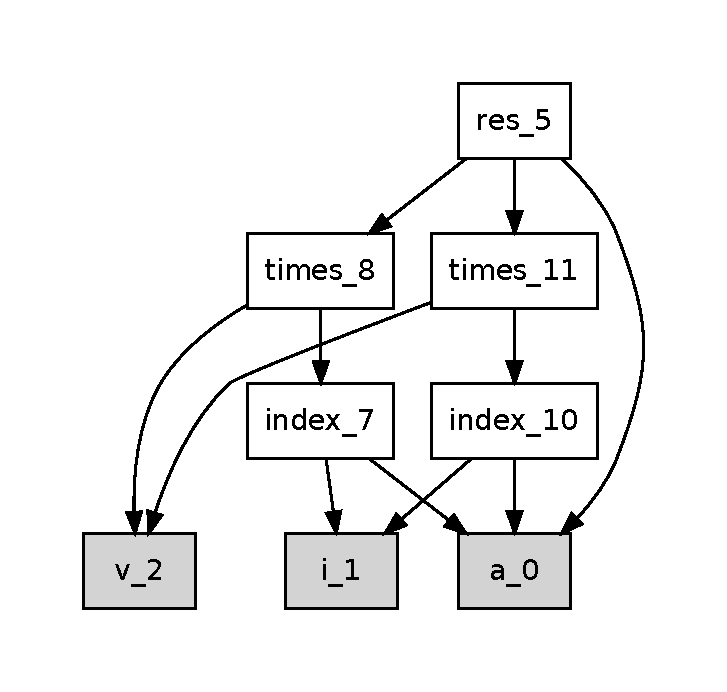
\includegraphics[width=4.5cm]{img/rebinder-ddg.pdf}
\caption{Data dependency graph for example program}
\label{fig:rebinder-example-graph}
\end{figure}

None of these bindings can be removed, as the names they bind may be
used in subexpressions, but their right-hand sides (RHS) can be
changed freely.  This is what is exploited to perform CSE.  The
following steps are performed:

\begin{description}
\item[\texttt{index\_10}:] Inserted unchanged, but we record its RHS,
  in case we end up seeing an identical expression later on.
\item[\texttt{times\_11}:] Likewise inserted unchanged, as its RHS
  does not correspond to any previously seen.
\item[\texttt{index\_7}:] Since the RHS of this binding is identical
  to the RHS of \texttt{index\_10}, we replace the RHS of
  \texttt{index\_7} with the variable \texttt{index\_10}.  We insert
  the resulting binding \texttt{let~times\_11~=~index\_7} and record
  the substitution $\texttt{index\_y}\rightarrow\texttt{index\_10}$.
\item[\texttt{times\_8}:] The substitution
  $\texttt{index\_y}\rightarrow\texttt{index\_10}$ is performed on the
  immediate subexpressions of the RHS, obtaining
  \texttt{v\_2~*~index\_10}, then check whether the resulting
  expression has been seen before.  This turns out to be identical to
  the RHS of \texttt{times\_11}, and therefore we insert the binding
  \texttt{let~times\_8~=~times\_11}.
\item[\texttt{res\_5}:] The substitution
  $\texttt{index\_y}\rightarrow\texttt{index\_10},\texttt{times\_8}\rightarrow\texttt{times\_11}$
  is performed, although no changes are made.  The binding is then
  inserted.
\end{description}

The result is the following program:

\begin{colorcode}
fun int main([int] a_0, int i_1, int v_2) =
  let index_10 = a_0[i_1] in
  let times_11 = v_2 * index_10 in
  let index_7 = index_10 in
  let times_8 = times_11 in
  let {res_5} =
    reduceT(fn \{int\} (int sum_3, int x_4) =>
              let plus_6 = sum_3 + x_4 in
              let plus_9 = plus_6 + times_8 in
              \{plus_9\},
            \{times_11\}, a_0) in
  res_5
\end{colorcode}

Copy propagation can then be used to remove the \texttt{index\_7} and
\texttt{times\_8} bindings.\fixme{This is still way too vague and hard to understand.}

\subsection{Hoisting Bindings}
\label{sec:hoisting-bindings}

The problem is as follows: We are given a potentially hoistable set,
$\{(p_{i}, e_{i})\}$, of patterns $p_{i}$ and $e_{i}$.  Each pattern
$p_{i}$ defines several names that may be used by other expressions in
the set.

We need to split the potentially hoistable set into a
\textit{hoistable set}, and a set of the bindings that cannot be
hoisted further, the \textit{unhoistable set}.  To this end, we are
given a unary relation $\mathcal{B}$, that given a binding $(p_{i},
e_{i})$, tells us whether $e_{i}$ is blocked from being hoisted.  As
the most archetypical reason, $\mathcal{B}(p_{i}, e_{i})$ whenever
$e_{i}$ uses a parameter of the function that we are trying to hoist
out of, but the relation also checks the other cases mentioned in
\cref{sec:when-not-to-hoist}.

Each of the expressions $e_{i}$ may use variables from any of the
patterns $p_{j}$ (except its own), but there may also be free
variables that are not contained in any pattern in the potentially
hoistable set.  These correspond to names bound higher up in the
program.

Since the potentially hoistable set is partially ordered, we can
process its elements in dependency order.  We keep track of the names
bound by unhoistable bindings in an \textit{unhoisted name set},
initially empty.  For each binding $(p_{i},e_{i})$, we check whether
$\mathcal{B}(p_{i},e_{i})$ or $e_{i}$ uses a name in the unhoisted
name set:
\begin{itemize}
\item If so, the binding is put into the unhoistable set, and the
  names in $p_{i}$ are added to the unhoisted name set.
\item Otherwise, the binding is put into the hoistable set.
\end{itemize}
The end result is a set of hoistable bindings, and a set of
nonhoistable bindings.  Because of the ordering, we are guaranteed
that no binding in the former uses a name bound in the
latter.\fixme{Insert figure}

\subsection{Inserting Bindings}

\fixme{Explain the ``insertion'' part.}

\subsection{Simplification of Expressions}
\label{sec:simplification-of-expressions}

The CSE technique described in previous sections depends heavily on
semantically identical code also having ($\alpha$-)equivalent
bindings.  However, in many cases, two expressions may have different
syntax trees, yet semantically be the same.  For example, consider the
expressions \texttt{(x*y)*z} versus \texttt{x*(y*z)}.  If we assume
that \texttt{*} is associative\footnote{Strictly not the case for
  floating-point multiplication.}, these expressions will always
compute the same value.  With respect to Anormalisation, the two
different normalised expressions are shown on
\cref{fig:differing-normalisation}.

\begin{figure}
\begin{subfigure}[t]{.33\textwidth}
\centering
\begin{colorcode}
let a = x * y in
let b = a * z in
b
\end{colorcode}
\subcaption{\texttt{(x * y) * z}}
\end{subfigure}%
\begin{subfigure}[t]{.33\textwidth}
\centering
\begin{colorcode}
let a = y * z in
let b * x * a in
b
\end{colorcode}
\subcaption{\texttt{x * (y * z)}}
\end{subfigure}%
\begin{subfigure}[t]{.33\textwidth}
\centering
\begin{colorcode}
let a = z * y in
let b * x * a in
b
\end{colorcode}
\subcaption{\texttt{x * (z * y)}}
\end{subfigure}
\caption{Normalisation of syntactically different expressions}
\label{fig:differing-normalisation}
\end{figure}

Despite the syntactical difference between these two expressions, they
are clearly semantically identical, and we would like for CSE to
remove one of them.  Given the way our CSE optimisation works, the
only solution is to ensure that equivalent expessions A-normalise to
$\alpha$-equivalent bindings.  In general, this is a very hard-problem
- in fact, determining whether two expressions will always evaluate to
the same result is undecideable, as it reduces to the halting problem.
Fortunately, the problem becomes quite tractable with restricted to
arithmetic operations, through the use of \textit{simplification}
before employing the normaliser.

One solution, which was implemented in an unpublished bachelors thesis
by Jonas Brunsgaard and Rasmus Wriedt Larsen, is to simplify
arithmetic expressions into a form known as \textit{sum-of-products}.
In this form, the top node of the syntax tree for an arithmetic
expression is always an addition node with $n$ multiplication
children.  Each of these multiplication nodes may have $m$ children,
which can be arbitary numeric expressions.  By ordering the children
of each node according to some criterion (say, lexicographically), we
obtain a unique tree structure for arithmetic expressions that ignores
superficial syntactical differences, such as one shown on
\cref{fig:differing-normalisation}.  This unique tree structure can
then be A-normalised into an equally unique set of bindings.

%%% Local Variables: 
%%% mode: latex
%%% TeX-master: "thesis.tex"
%%% End: 


\chapter{The Rebinder}
\label{chap:rebinder}

In the compiler literature, \textit{hoisting} (also known as
\textit{loop-invariant code motion}) is the movement of loop-invariant
expressions out of a loop.  This has a clear benefit: rather than
executing once per iteration of the loop, the expression is executed
once before the loop begins.  For \LO{}, hoisting can be an important
optimisation, as it holds the potential for moving bounds checks and
other assertions out of inner loops.  We will see an example of this
in the next section.

Common Subexpression Elimination (henceforth referred to as CSE) is a
popular compiler optimisation that identifies identical expressions
(i.e. expressions that always evaluate to the same value), and
replaces them with a variable holding the computed value.  If the
common expressions are expensive or computed very frequently, e.g. by
being part of an inner loop, this can result in significant speedup.

It turns out that hoisting and common subexpression elimination can be
unified in a single framework, which in the \LO{} compiler is termed
the \textit{Rebinder}.

This chapter will start out by describing basic principles of hoisting
and CSE in \cref{sec:hoisting,sec:cse}.  In \cref{sec:rebinder}, we
will describe their implementation in the \LO{} compiler.

\section{Hoisting}
\label{sec:hoisting}

When compiling an imperative language,
we must be careful not to move any code with side effects, but in a
pure language such as \LO{}, we can hoist freely (with a few
restrictions that I'll get to in \cref{sec:when-not-to-hoist}).  A
simple example of hoisting in action is shown on
\cref{fig:simple-hoisting}.

\begin{figure}
\begin{center}
\begin{bcolorcode}
map(fn int (int x) =>
      let k = y + z in
      x + k,
    a)
\end{bcolorcode}
\hspace{1cm}
\adjustbox{valign=t}{
\(\Rightarrow\)
}%
\hspace{1cm}
\begin{bcolorcode}
let k = y + z in
map(fn int (int x) =>
      x + k,
    a)
\end{bcolorcode}
\end{center}

\caption{Hoisting in action}
\label{fig:simple-hoisting}
\end{figure}

At first glance, hoisting may seem to apply too rarely to be of much
benefit, since most programmers would put loop-invariant code outside
of the loop in the first place.  However, there are two important use
cases that do not involve programmer-written code:

\begin{itemize}
\item Much \LO{} code is not written by the programmer, but is rather
  the result of program transformation by the compiler.  Inlining and
  constant folding may easily result in the creation of loop-invariant
  expressions within a loop.

\item Explicit bounds checks, as introduced in \cref{sec:assertions},
  can sometimes be hoisted out of inner loops.
\end{itemize}

The latter case merits futher elaboration.  Consider the following
program:

\begin{colorcode}
map(fn int (int i) =>
      a[i] + a[i*2],
    iota(n))
\end{colorcode}

Here, \texttt{a} is a free variable.  Once the compiler has turned the
implicit bound checks explicit, the program will look like this:

\begin{colorcode}
map(fn int (int i) =>
      let c1 = assert(i   >= 0 && i   < size(0,a)) in
      let c2 = assert(i*2 >= 0 && i*2 < size(0,a)) in
      a[<c1>|i] + a[<c2>|i*2],
    iota(n))
\end{colorcode}

Now, the assertions are not loop-invariant, as they depend on
\texttt{i}.  If we assume a sufficiently smart compiler, for example
by employing some extension of \textit{symbolic range
  propagation}\cite{blume1995symbolic}, we can deduce that the
variable \textit{i} will always be in the range $[0,n-1]$.  This
allows us to rewrite the assertions -- the checks for non-negativity
goes away, as it is always true, and we only have to check the upper
bound for the maximum values that \texttt{i} and \texttt{i*2} may
attain:

\begin{colorcode}
map(fn int (int i) =>
      let c1 = assert(n   < size(0,a)) in
      let c2 = assert(n*2 < size(0,a)) in
      a[<c1>|i] + a[<c2>|i*2],
    iota(n))
\end{colorcode}

Now \texttt{c1} and \texttt{c2} are loop-invariant, and we can move
them out of the loop body, and perform bounds checking just once,
before entering the loop:

\begin{colorcode}
let c1 = assert(n   < size(0,a)) in
let c2 = assert(n*2 < size(0,a)) in
map(fn int (int i) =>
      a[<c1>|i] + a[<c2>|i*2],
    iota(n))
\end{colorcode}

For a simple loop such as the above, the potential benefits are great,
as most of the instructions of the original loop body was devoted to
bounds checkings.

The \LO{} compiler does not yet support the range analysis that
enables the critical rewrite of the \texttt{assert} expressions.  An
unpublished bachelors thesis by Jonas Brunsgaard and Rasmus Wriedt
Larsen suggests that the technique works in practice, but their work
has not yet been merged with the main compiler code base.

Hoisting assertions such as these is useful not only when the program
uses explicit array indexing.  While the array accesses performed by
SOACs are by construction always in-bounds, and therefore do not need
dynamic checks, the \texttt{assert} expressions we generate when
transforming from external SOACs to tupleless SOACs are conceptually
identical to bounds checks, and similarly important to hoist.  For
example, consider this program:

\begin{colorcode}
map(fn [int] ([int] r) =>
      map(op+, zip(r, b)),
    a)
\end{colorcode}

After transformation to internal \LO{}, we get the following:

\begin{colorcode}
mapT(fn \{[int]\} ([int] r) =>
       let c = assert(size(0,r) = size(0,b)) in
       <c>mapT(op+, r, b),
    a)
\end{colorcode}

The assertion is not loop-invariant, and range analysis is no help.
For this case, structural size analysis (described in depth in
\cref{sec:size-analysis}) reveals that since \texttt{r} is a row of
\texttt{a}, the outer size of \texttt{r} (\texttt{size(0,r)}) is equal
to the inner size of \texttt{a} (\texttt{size(1,a)}).  Thus, the
compiler rewrites to:

\begin{colorcode}
mapT(fn \{[int]\} ([int] r) =>
       let c = assert(size(1,a) = size(0,b)) in
       <c>mapT(op+, r, b),
    a)
\end{colorcode}

The assertion is now loop-invariant and can be hoisted:

\begin{colorcode}
let c = assert(size(1,a) = size(0,b)) in
mapT(fn \{[int]\} ([int] r) =>
       <c>mapT(op+, r, b),
    a)
\end{colorcode}

The details of how hoisting is implemented in the \LO{} compiler is
covered in \cref{sec:rebinder}.

\subsection{What Not to Hoist}
\label{sec:when-not-to-hoist}

Clearly, we can hoist only loop-invariant expressions.  Unfortunately,
not all loop-invariant expressions are hoistable, and as is often the
case when seemingly valid transformations become problematic,
constraints imposed by uniqueness types are at fault.  Consider the
following program:

\begin{colorcode}
map(fn (int i) =>
      let a = iota(10) in
      f(a, i),
    b)
\end{colorcode}

It seems that we should be able to hoist \texttt{a} out of the loop
like this:

\begin{colorcode}
let a = iota(10) in
map(fn (int i) =>
      f(a, i),
    b)
\end{colorcode}

However, if the function call \texttt{f(a,i)} consumes the \texttt{a}
argument, hoisting would result in an invalid program, as \texttt{a}
would be consumed multiple times.  We need a ``freshly allocated''
\texttt{a} for each iteration of the loop.  Hence, we must not hoist a
binding out of a loop in which it is consumed.

As a minor, but important point, it is strictly not permitted to hoist
out of loops unless it can be proven that the loop will always execute
at least one iteration.  The \LO{} compiler currently ignores this
restriction, implicitly assuming that all arrays are non-empty.

\subsubsection{Hoisting out of branches}

Most compilers generally do not hoist out of branches, as branching is
often used to prevent expensive execution of expensive expressions
whose value is not needed.  On many GPUs however, execution happens in
lock-step across all processors.  This implies that unless the branch
condition computes the same value in all threads, both sides of the
branch will have to be executed~\cite{reducing-branch-divergence}.
This implies that in some cases, hoisting out of a branch does not
cause more instructions to be executed, and hoisting might expose the
possibility of other optimisations, particularly common subexpression
elimination (see \cref{sec:cse}).

We should still be careful when hoisting expressions out of the
branches of a conditional, as it is possible that the expression may
result in an error unless the condition checked by the conditional is
true.  For example, consider this expression:

\begin{colorcode}
if \(c\) then y / x
     else if \(p\) then y / x
               else 0
\end{colorcode}

If \texttt{y / x} was hoisted out of the branch, the resulting program
might end up dividing by zero.  Assertions and array indexing are
other operations that are not safe to hoist out of a branch.  Most
expressions are safe however, and the \LO{} compiler aggressively
hoists these out of branches.  Depending on improvements in hardware,
or the targeting of \LO{} for non-GPU systems, it is likely that this
strategy will need to be revised.

\subsubsection{Performance Considerations}

There is another potential case where hoisting, while not resulting in
an invalid program, proves detrimental rather than beneficial to
performance.  This occurs when retrieving the hoisted value from
memory would be more expensive than re-computing it for each loop
iteration, which is particularly likely to occur on GPUs, as global
memory accesses are enormously expensive.  Balancing this problem is
not currently tackled by the \LO{} compiler, which instead hoists as
aggressively as possible.  Note that this is not a problem when
hoisting assertions, such as bounds checks, as the resulting values
are not actually accessed from within the loop.

\section{Common Subexpression Elimination}
\label{sec:cse}

Common Subexpression Elimination (henceforth referred to as CSE) is a
popular compiler optimisation that identifies identical expressions
(i.e. expressions that always evaluate to the same value), and
replaces them with a variable holding the value.  For example, this
program:

\begin{colorcode}
2 * x + 2 * x
\end{colorcode}

Can be transformed through CSE into:

\begin{colorcode}
let tmp = 2 * x in
tmp + tmp
\end{colorcode}

This saves us a multiplication.  As with hoisting, CSE can potentially
be detrimental to performance if it increases memory pressure, but
again like hoisting, this is not something the \LO{} compiler
currently takes into consideration.

We must be careful not to perform CSE such that we end with a
violation of the uniqueness rules.  Consider this program:

\begin{colorcode}
let a = iota(10) in
let b = iota(10) in
let a[2] = 5 in
f(a,b)
\end{colorcode}

Since \texttt{iota(10)} appears in two places, we might be tempted to
factor it out:

\begin{colorcode}
let tmp = iota(10) in
let a = tmp in
let b = tmp in
let a[2] = 5 in
f(a,b)
\end{colorcode}

However, this violates Uniqueness Rule 1, as \texttt{b} is aliased to
\texttt{a}, yet is used after \texttt{a} is consumed in a
\texttt{let-with} expression.  The solution is to not perform CSE on
expressions whose result is eventually consumed -- or more
conservatively, never perform CSE on an expression of type
\texttt{*[$\alpha$]}.  The latter is easier to implement, although too
conservative, but is what the \LO{} compiler currently does.

\section{Rebinder Implementation}
\label{sec:rebinder}

Conceptually, hoisting and CSE are rather different transformations.
However, they both depend on identifying subexpressions that can be
moved (in the case of hoisting) or replaced (in the case of CSE), but
where the actual expression rewriting is quite simple.  In the \LO{}
compiler, the observation was made that a lot of the machinery used to
implement hoisting could be easily extended to also perform CSE, and
thus was born a compiler pass with the rather idiosyncratic name
\textit{the Rebinder}.

The central idea is to assume a program in a slightly modified
A-normal form~\cite{Sabry:1992:RPC:141478.141563}, a format similar to
\textit{three address code}, where the definition of each
\texttt{let}-binding is a \textit{simple expression}, and the body of
a \texttt{let}-binding is either another binding or a variable.  A
simple expression is either a branch\footnote{Not permitted in
  ``standard'' A-normal form.}, or an expression where all
subexpressions are variables or constants (except for the bodies of
SOAC functions), which implies that their execution terminates
immediately.  For example, the following program:

\begin{colorcode}
fun real solve(real a, real b, real c) =
  (-b + sqrt(b*b - 4.0*a*c)) / (2.0*a)
\end{colorcode}

Would look like this in A-normal form.  Note that it is also
\texttt{let}-normalised (\cref{sec:let-normalisation}):

\begin{colorcode}
fun real solve(real a_0, real b_1, real c_2) =
  let negate_3  = -b_1 in
  let times_4   = b_1 * b_1 in
  let times_5   = 4.0 * a_0 in
  let times_6   = times_5 * c_2 in
  let minus_7   = times_4 - times_6 in
  let norm_8    = sqrt(minus_7) in
  let plus_9    = negate_3 + norm_8 in
  let times_10  = 2.0 * a_0 in
  let divide_11 = plus_9 / times_10 in
  divide_11
\end{colorcode}

This simplifies hoisting and CSE significantly, as the problem is now
reduced to moving nodes in the syntax tree (for hoisting) and
substituting definitions of \texttt{let}-bindings (for CSE).
A-normalisation is performed by a separate pass before entering the
Rebinder, and is generally trivial, but there are a few difficulties
that I will cover in \cref{sec:simplification-of-expressions}.

In order to keep the exposition simpler, \texttt{loop} and
\texttt{let-with} will be ignored (except with respect to upholding
uniqueness constraints), and only discuss hoisting of normal
\texttt{let}-bindings.

To try to give an intuition of the Rebinder, let us consider the
following contrived program:

\begin{colorcode}
fun int main([int] a, int i, int v) =
  let {res} =
    reduceT(fn \{int\} (int sum, int x) =>
              {sum + x + v*a[i]},
            \{v*a[i]\}, a) in
  res
\end{colorcode}

The goal is to hoist the loop-invariant expression \texttt{v*a[i]} out
of the loop, and use CSE to combine it with the initial value of the
accumulator.  To this end, it is first transformed to A-normal form:

\begin{colorcode}
fun int main([int] a_0, int i_1, int v_2) =
  let index_10 = a_0[i_1] in
  let times_11 = v_2 * index_10 in
  let \{res_5\} =
    reduceT(fn \{int\} (int sum_3, int x_4) =>
              let plus_6 = sum_3 + x_4 in
              let index_7 = a_0[i_1] in
              let times_8 = v_2 * index_7 in
              let plus_9 = plus_6 + times_8 in
              {plus_9},
            \{times_11\}, a_0) in
  res_5
\end{colorcode}

The intuition we will use is to strip an expression $e$ of any
enclosing bindings, resulting in a ``core'' expression $e'$, and a set
of bindings.  There may be free variables in $e'$ that are bound by
the bindings in the set.  At some point, we will have to insert the
bindings in the program, but we will try to put them as far up the
syntax tree as possible.  For example, stripping the body of
\texttt{main} above would result in the core expression
\texttt{res\_5} and the bindings \texttt{index\_10},
\texttt{times\_11}, and \texttt{res\_5}.

The set of bindings, which we will term the \textit{potentially
  hoistable set}, is a partially ordered set of binding pairs
$(p_{i},e_{i})$.  A binding pair $(p_{i},e_{i})$ corresponds to the
\LO{} binding \texttt{let~$p_{i}$~=$e_{i}$}.  The partial order is
$\preceq$: for two bindings $b_{i}, b_{j}$, $b_{i} \preceq b_{j}$ if
$b_{j}$ uses any variables bound by $b_{i}$, or if $b_{i} = b_{j}$.
The potentially hoistable set thus represents an acyclic
data-dependency graph.

The Rebinder proceeds with a recursive walk down the syntax tree,
collecting bindings into the potentially hoistable set.  Additionally,
for each binding, we recurse down its right-hand side in order to
determine whether it contains any \textit{hoistable subexpressions}.
This is only the case if the RHS is a SOAC -- where we can hoist out
of the body -- or \texttt{if} -- where we can hoist out of the
branches.  For all other expressions, due to the program being in
A-normal form, the subexpressions will be variables or constants,
which are not hoisted.

A traversal of the example program listed above follows:

\begin{itemize}
\item First, we encounter the \texttt{index\_10} and
  \texttt{times\_11} bindings, and their right-hand sides are
  inspected.  Neither of these inspections yield hoistable
  subexpressions, but we remove \texttt{index\_10} and
  \texttt{index\_11} themselves and insert them into the potentially
  hoistable set.

\item Next, we encounter the \texttt{res\_5} binding and we descend
  recursively into the scope of the SOAC function body:

  \begin{itemize}
  \item We inspect the right-hand sides of \texttt{plus\_6},
    \texttt{index\_7}, \texttt{times\_8} and \texttt{plus\_9}, none of
    which yield hoistable subexpressions.  We collect these bindings
    into a potentially hoistable set and remove them from the function
    body, leaving just the expression \texttt{\{plus\}}.

  \item We are now done inspecting the function, and we need to decide
    which of the bindings in the potentially hoistable set can in fact
    be hoisted out.  The function parameters are \texttt{sum\_3} and
    \texttt{x\_4}, and any bindings that depend on these cannot be
    hoisted (the details are given in \cref{sec:hoisting-bindings}).
    This leaves the bindings for \texttt{index\_7} and
    \texttt{times\_8} as hoistable; while \texttt{plus\_6} and
    \texttt{plus\_9} are re-inserted into the program.
  \end{itemize}

  This yields the \texttt{index\_7} and \texttt{times\_8} bindings as
  new elements in the potentially hoistable set.  We also add the
  modified \texttt{res\_5} binding itself.

\item Since there are no more bindings left, and we are at the top
  level of a function, we insert the bindings in the potentially
  hoistable set (\texttt{index\_10}, \texttt{times\_11},
  \texttt{res\_5}, \texttt{index\_7} and \texttt{times\_8}) in the
  program, yielding:

\begin{colorcode}
fun int main([int] a_0, int i_1, int v_2) =
  let index_10 = a_0[i_1] in
  let times_11 = v_2 * index_10 in
  let index_7 = a_0[i_1] in
  let times_8 = v_2 * index_7 in
  let {res_5} =
    reduceT(fn \{int\} (int sum_3, int x_4) =>
              let plus_6 = sum_3 + x_4 in
              let plus_9 = plus_6 + times_8 in
              \{plus_9\},
            \{times_11\}, a_0) in
  res_5
\end{colorcode}
\end{itemize}

We could now do a separate CSE pass over the entire program, but there
may be a more efficient strategy.  The Rebinder is able to perform the
CSE optimisation whenever we insert the non-hoistable bindings into
the syntax tree.  We will try to provide an intuition for the
approach, using the above example:

When, at the end, we have to insert bindings for \texttt{index\_10},
\texttt{times\_11}, \texttt{res\_5}, \texttt{index\_7} and
\texttt{times\_8}, we have to determine an order that does not result
in a variable being used before it is defined.  This is easy, since
the potentially hoistable set is already dependency-ordered and thus
defines a data dependency graph (shown on
\cref{fig:rebinder-example-graph}).  The following insertion order is
obtained by performing a depth-first traversal of the graph:

\begin{enumerate}
\item \texttt{index\_10}
\item \texttt{times\_11}
\item \texttt{index\_7}
\item \texttt{times\_8}
\item \texttt{res\_5}.
\end{enumerate}

\begin{figure}
\centering
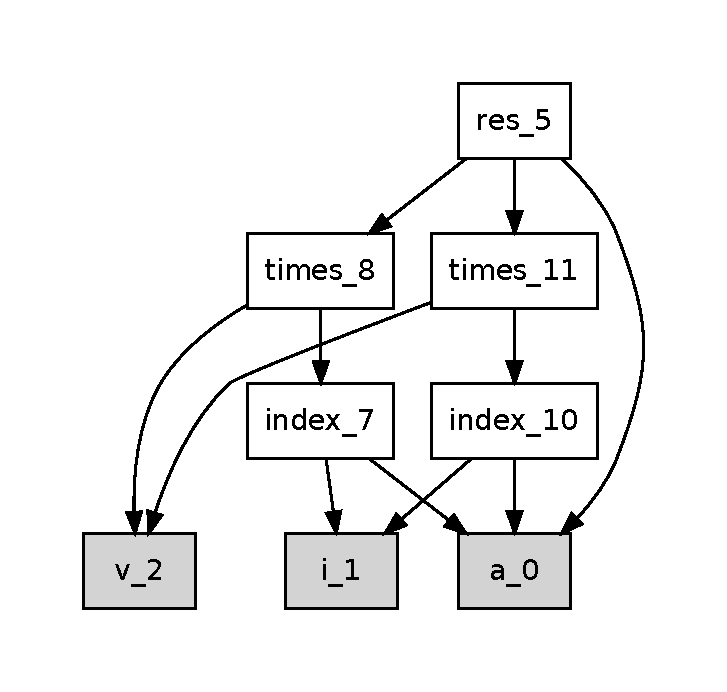
\includegraphics[width=4.5cm]{img/rebinder-ddg.pdf}
\caption{Data dependency graph for example program}
\label{fig:rebinder-example-graph}
\end{figure}

None of these bindings can be removed, as the names they bind may be
used in subexpressions, but their right-hand sides (RHS) can be
changed freely.  This is what is exploited to perform CSE.  The
following steps are performed:

\begin{description}
\item[\texttt{index\_10}:] Inserted unchanged, but we record its RHS,
  in case we end up seeing an identical expression later on.
\item[\texttt{times\_11}:] Likewise inserted unchanged, as its RHS
  does not correspond to any previously seen.
\item[\texttt{index\_7}:] Since the RHS of this binding is identical
  to the RHS of \texttt{index\_10}, we replace the RHS of
  \texttt{index\_7} with the variable \texttt{index\_10}.  We insert
  the resulting binding \texttt{let~times\_11~=~index\_7} and record
  the substitution $\texttt{index\_y}\rightarrow\texttt{index\_10}$.
\item[\texttt{times\_8}:] The substitution
  $\texttt{index\_y}\rightarrow\texttt{index\_10}$ is performed on the
  immediate subexpressions of the RHS, obtaining
  \texttt{v\_2~*~index\_10}, then check whether the resulting
  expression has been seen before.  This turns out to be identical to
  the RHS of \texttt{times\_11}, and therefore we insert the binding
  \texttt{let~times\_8~=~times\_11}.
\item[\texttt{res\_5}:] The substitution
  $\texttt{index\_y}\rightarrow\texttt{index\_10},\texttt{times\_8}\rightarrow\texttt{times\_11}$
  is performed, although no changes are made.  The binding is then
  inserted.
\end{description}

The result is the following program:

\begin{colorcode}
fun int main([int] a_0, int i_1, int v_2) =
  let index_10 = a_0[i_1] in
  let times_11 = v_2 * index_10 in
  let index_7 = index_10 in
  let times_8 = times_11 in
  let {res_5} =
    reduceT(fn \{int\} (int sum_3, int x_4) =>
              let plus_6 = sum_3 + x_4 in
              let plus_9 = plus_6 + times_8 in
              \{plus_9\},
            \{times_11\}, a_0) in
  res_5
\end{colorcode}

Copy propagation can then be used to remove the \texttt{index\_7} and
\texttt{times\_8} bindings.

\subsection{Hoisting Bindings}
\label{sec:hoisting-bindings}

The problem is as follows: We are given a potentially hoistable set,
$\{(p_{i}, e_{i})\}$, of patterns $p_{i}$ and $e_{i}$.  Each pattern
$p_{i}$ defines several names that may be used by other expressions in
the set.

We need to split the potentially hoistable set into a
\textit{hoistable set}, and a set of the bindings that cannot be
hoisted further, the \textit{unhoistable set}.  To this end, we are
given a unary relation $\mathcal{B}$, that given a binding $(p_{i},
e_{i})$, tells us whether $e_{i}$ is blocked from being hoisted.  As
the most archetypical reason, $\mathcal{B}(p_{i}, e_{i})$ whenever
$e_{i}$ uses a parameter of the function that we are trying to hoist
out of, but the relation also checks the other cases mentioned in
\cref{sec:when-not-to-hoist}.  We will consider as unhoistable any
binding that is unhoistable according to $\mathcal{B}$, as well as any
binding that depends on an unhoistable binding.

Each of the expressions $e_{i}$ may use variables from any of the
patterns $p_{j}$ (except its own), but there may also be free
variables that are not contained in any pattern in the potentially
hoistable set.  These correspond to names bound higher up in the
program.

Since the potentially hoistable set is partially ordered, we can
process its elements in dependency order.  We keep track of the names
bound by unhoistable bindings in an \textit{unhoisted name set},
initially empty.  For each binding $(p_{i},e_{i})$, we check whether
$\mathcal{B}(p_{i},e_{i})$ or $e_{i}$ uses a name in the unhoisted
name set:
\begin{itemize}
\item If so, the binding is put into the unhoistable set, and the
  names in $p_{i}$ are added to the unhoisted name set.
\item Otherwise, the binding is put into the hoistable set.
\end{itemize}
The end result is a set of hoistable bindings, and a set of
nonhoistable bindings.  Because of the ordering, we are guaranteed
that no binding in the former uses a name bound in the
latter.

\subsection{Inserting Bindings}

After dividing the potentially hoistable set into hoistable and
non-hoistable bindings, we have to insert all non-hoistable bindings
around the core expression.  Concretely, we are given a core
expression $e_{c}$ and an ordered set of expressions
$\{(p_{i},~e_{i})\}$, where binding $(p_{i},~e_{i})$ must precede
binding $(p_{i+1},~e_{i+1})$.  We can take this opportunity to perform
dead code elimination by removing any binding $(p_{i},~e_{i})$ that is
not used in either $e_{c}$ or any enclosed binding.  The idea is to
track which names are actually used in the lexical scope of the
binding, and remove bindings that are never referenced.

The algorithm is as follows.  We will track two pieces of data: A set
$\mathcal{F}$, which is initialised to the free variables of $e_{c}$
\footnote{This can be done efficiently if the rebinder constantly
  tracks the free variables of the core expression.}.  Then we proceed
\textit{backwards} through the list of bindings, i.e., we first
process the binding that should be innermost.  For each binding
$(p_{i},~e_{i})$, we check whether any of the names bound by $p_{i}$
are present in $\mathcal{F}$.  If so, we add the free variables of
$e_{i}$ to $\mathcal{F}$ and insert the binding.  If the binding is
not used, we skip it.

\subsection{Simplification of Expressions}
\label{sec:simplification-of-expressions}

The CSE technique described in the previous sections depends heavily
on semantically identical code also having ($\alpha$-)equivalent
bindings.  However, in many cases, two expressions may have different
syntax trees, yet semantically be the same.  For example, consider the
expressions \texttt{(x*y)*z} versus \texttt{x*(y*z)}.  If we assume
that \texttt{*} is associative\footnote{Strictly not the case for
  floating-point multiplication.}, these expressions will always
compute the same value.  With respect to A-normal form, the two
different normalised expressions are shown on
\cref{fig:differing-normalisation}.

\begin{figure}
\begin{subfigure}[t]{.33\textwidth}
\centering
\begin{colorcode}
let a = x * y in
let b = a * z in
b
\end{colorcode}
\subcaption{\texttt{(x * y) * z}}
\end{subfigure}%
\begin{subfigure}[t]{.33\textwidth}
\centering
\begin{colorcode}
let a = y * z in
let b * x * a in
b
\end{colorcode}
\subcaption{\texttt{x * (y * z)}}
\end{subfigure}%
\begin{subfigure}[t]{.33\textwidth}
\centering
\begin{colorcode}
let a = z * y in
let b * x * a in
b
\end{colorcode}
\subcaption{\texttt{x * (z * y)}}
\end{subfigure}
\caption{Normalisation of syntactically different expressions}
\label{fig:differing-normalisation}
\end{figure}

Despite the syntactical difference between these two expressions, they
are clearly semantically identical, and we would like for CSE to
remove one of them.  Given the way our CSE optimisation works, the
only solution is to ensure that equivalent expessions A-normalise to
$\alpha$-equivalent bindings.  In general, this is a very hard-problem
- in fact, determining whether two expressions will always evaluate to
the same result is undecideable, as it reduces to the halting problem.
Fortunately, the problem becomes quite tractable with restricted to
arithmetic operations, through the use of \textit{simplification}
before employing the normaliser.

One solution, which was implemented in an unpublished bachelors thesis
by Jonas Brunsgaard and Rasmus Wriedt Larsen, is to simplify
arithmetic expressions into a form known as \textit{sum-of-products}.
In this form, the top node of the syntax tree for an arithmetic
expression is always an addition node with $n$ multiplication
children.  Each of these multiplication nodes may have $m$ children,
which can be arbitary numeric expressions.  By ordering the children
of each node according to some criterion (say, lexicographically), we
obtain a unique tree structure for arithmetic expressions that ignores
superficial syntactical differences, such as one shown on
\cref{fig:differing-normalisation}.  This unique tree structure can
then be A-normalised into an equally unique set of bindings.

%%% Local Variables: 
%%% mode: latex
%%% TeX-master: "thesis.tex"
%%% End: 


\chapter{Fusion}
\label{chap:fusion}

This chapter will outline the principles behind
\textit{producer-consumer} loop fusion, describe their implementation
in the \LO{} compiler, and discuss possible complications and
restrictions of my handling of loop fusion.

In producer-consumer fusion, the aim is to merge (or \textit{fuse})
two loops, where the output of the first loop -- the producer -- is
used as input to the second -- the consumer.  We currently only fuse
loops that are expressed via SOACs, not the \texttt{do}-notation.  The
reason for this is to simplify analysis, as it can be hard to
determine in which cases arbitrary \texttt{do}-loops can be combined,
whereas it is possible to define simple rules for how and when SOACs
can be fused.

As a simple case, we can fuse the two loops in
\[
\texttt{(map~$f$)~$\circ$~(map~$g$)}
\]
and get
\[
\texttt{map~$(f~\circ~g)$},
\]
thus removing the need to construct an intermediary array for the
result of \texttt{map~$g$}, and in the context of GPGPU, reducely the
likelyhood of global memory accesses.  We will write ``$c_{1}$-$c_{2}$
fusion'' for the case where a fusion is formed with $c_{1}$ as the
producer and $c_{2}$ as the consumer.  Therefore, the previous example
would be ``\texttt{map}-\texttt{map}''-fusion.

\section{Fusion in \LO{}}

The language used to describe the fusion algorithm in this chapter is
\texttt{let}-normalised, internal \LO{}, as described in chapter
\ref{chap:internal}.  We will also assume that all instances of
\texttt{replicate(n,x)} have been rewritten as
\texttt{map(fn~t~(int~i)~=>~x,~iota(n))}.  For clarity, expository
examples will use the external \LO{}.

\begin{figure}
  \begin{center}
    \begin{tabular}{c|c}
      \textbf{Producers} & \textbf{Consumers} \\\hline
      \texttt{map} & \texttt{map} \\\hline
      & \texttt{reduce} \\\hline
      \texttt{scan} & \texttt{scan} \\\hline
      \texttt{filter} & \texttt{filter} \\\hline
      & \texttt{redomap} \\\hline
    \end{tabular}
  \end{center}
  \caption{Producers and consumers in \LO}
  \label{fig:producers-consumers}
\end{figure}

\fref{fig:producers-consumers} lists which \LO{} SOACs are producers,
which are consumers, and which are both.  In particular, note that
even if we have a \texttt{reduce}-expression returning an array, this
does not mean that the \texttt{reduce}-expression is a producer - it
can under no circumstances be fused into another SOAC-expression.  The
reason is that the output of the reduction is only fully known after
the final input array element has been processed.  Consider the
following program:

\begin{colorcode}
let b = reduce(fn [int] ([int] acc, int x) =>
                 map(op + (x), acc),
               iota(10), a) in
map(f, b)
\end{colorcode}

The contents of the array \texttt{b} is not determined until the very
last element of \texttt{a} has been processed, and thus fusion with
the \texttt{map}-expression cannot take place.  While it is possible
to use \texttt{reduce} in a way that could theoretically be fused with
a consumer (for example by using it to simulate \texttt{map}), the
analysis necessary to determine whether a given reduction is fusable
would be quite onerous, and likely not useful in any but contrived
examples, such as the above-mentioned simulation of \texttt{map}.

In this way, \texttt{reduce} differs from \texttt{map}, in which each
element of the output is calculated from one element of the input ---
a classic case of data-parallelism.

Even if we have a producer-consumer-pair, not all such pairs
\textit{can} be fused, and not all are \textit{desirable} to fuse.
For instance, \texttt{filter}-\texttt{map} fusion is not possible,
although \texttt{filter}-\texttt{reduce} is.  The reason is that the
size of the \texttt{map}-output is the same as the size of its input,
yet the size of the output of \texttt{filter} cannot be known in
advance, which preclude an efficient fused form.

The \textit{fusion algebra} in section \ref{sec:fusionalgebra}
describes in detail which producer-consumer pairs can be fused, as
well as the form of the resulting SOAC.

Section \ref{sec:invalidfusion} goes into greater detail on invalid
fusion, and section \ref{sec:whentofuse} covers cases in which fusion
may actually be detrimental to performance.

...

My structural analysis is rooted in the
T$_{1}$-T$_{2}$-transformation~\cite{red_dragon}.\fxnote{Insert more
  about the transformation.}

\section{Invalid fusion}
\label{sec:invalidfusion}

We must be careful not to run afoul of uniqueness constraints when
doing fusion.  For example, consider the following program.

\begin{colorcode}
let b = map(f, a) in
let c = a with [i] <- x in
map(g, b)
\end{colorcode}

Without the contraints imposed upon us by the semantics of in-place
modification, we could fuse to the following program.

\begin{colorcode}
let c = a with [i] <- x in
map(g \(\circ\) f, a)
\end{colorcode}

However, this results in a violation of Uniqueness Rule 1, and the
resulting program is thus invalid.  In general, we must track the
possible execution paths from the producer-SOAC to the consumer-SOAC,
and only fuse if none of the inputs of the producer have been consumed
(in the uniqueness type sense of the word) by a \texttt{let-with} or
function call on any possible execution paths.

\section{When to fuse}
\label{sec:whentofuse}

Even when fusion is possible, it may not be beneficial, and may be
harmful to overall performance in the following cases.

\begin{description}[style=nextline]
\item[Computation may be duplicated.]

In the program
\begin{colorcode}
let x = map(f, a) in
\{map(g, x), map(h, x)\}
\end{colorcode}
fusing the \texttt{x}-producer into the two consumers will double the
number of calls to the function \texttt{f}, which might be expensive.
The implementation in the \LO{} compiler will currently only fuse if
absolutely no computation is duplicated, although this is likely too
conservative.  Duplicating cheap work, for example functions that use
only primitive operations on scalars, is probably not harmful to
overall performance, although I have not investigated this
fully.\fxnote{Reference someone who has.}

In general, in the context of GPU, the tradeoff between duplicating
computation and increasing communication is not an easy problem to
solve.  Accessing global memory can be more than a hundred times
slower than accessing local (register) memory, hence duplicating
computation is in many cases preferable.

\item[Can reduce memory locality.]

  Consider a simple case of fusing
  \texttt{(map~$f$)~$\circ$~(map~$g$)}.  When $g$ is executed for an
  element of the input array, neighboring elements will be put into
  the cache, making them faster to access.  This exhibits good data
  locality.  In contrast, the composed function $f~\circ~g$ will
  perform more work after accessing a given input element, increasing
  the risk that the input array may be evicted from the cache before
  the next element is to be used.  On GPUs, there is the added risk of
  the kernel function exercising additional register pressure, which
  may reduce hardware occupancy (thus reducing latency hiding) by
  having fewer computational cores active.  In this case, it may be
  better to execute each of the two \texttt{map}s as separate kernels.

  The \LO{} compiler does not currently handle this problem, as it is
  envisioned that a later (and as-of-yet unimplemented) transformation
  will perform \textit{loop distribution} (sometimes called
  \textit{loop fission}).  This step is necessary in any case, as it
  can be used to improve the degree of parallelism, compared to the
  original program.  \fref{fig:loop-distribution} demonstrates a fully
  fused \texttt{map} where the degree of parallelism is can be
  improved by distributing the inner reductions out of the loop.  In
  the original program, the inner map had to wait for the two
  reductions to finish computing \texttt{x} and \texttt{y} before
  executing its inner loop, whereas the distributed program consists
  of three parallel loop nests.
\end{description}

\begin{figure}
\begin{center}
\begin{bcolorcode}
map(fn int ([int] r) =>
      let x = reduce(f, 0, r) in
      let y = reduce(g, 0, r) in
      map(h(x,y), r),
    a)
\end{bcolorcode}

$\Downarrow$

\begin{bcolorcode}
let xs = map(reduce(f,0),a) in
let ys = map(reduce(g,0),a) in
map(fn [int] (\{int,int,[int]\} t) =>
      let \{r,x,y\} = t in
      map(h(x,y), r),
    zip(a,xs,ys))
\end{bcolorcode}
\end{center}
\caption{Loop distribution}
\label{fig:loop-distribution}
\end{figure}

\section{Composition}

\newcommand\mapcompose[7]{ (#1,#2) \underset{\texttt{map}}{\overset{#3}\circ}(#4,#5) \Rightarrow (#6,#7) }
\newcommand\filtercompose[7]{ (#1,#2) \underset{\texttt{filter}}{\overset{#3}\circ}(#4,#5) \Rightarrow (#6,#7) }
\newcommand\foldcompose[7]{ (#1,#2) \underset{\texttt{fold}}{\overset{#3}\circ}(#4,#5) \Rightarrow (#6,#7) }
\newcommand\inputmapping[0]{\mathcal{I}}
\newcommand\arrparams[1]{\textrm{params}(#1)}

To begin our discussion of the precise mechanics of fusion, I will
present the mechanics behind composing the functions involved in a
fusion operation.  For example, consider the trivial example of
\texttt{map}-\texttt{map}-fusion.  In principle, the equation seems
simple enough:
\[
\texttt{map}\ f \circ \texttt{map}\ g = \texttt{map}\ (f \circ g).
\]
However, while the intuition behind the above equation is correct, it
is woefully imprecise.  Fusion in \LO{} is not performed on simple
\texttt{map}s that take input from only one other \texttt{map}, but
complex \texttt{mapT}s that may take input from several sources, where
only some may be fusable.  Hence, a more detailed elaboration is
necessary.

In this section, we will assume that each output of a producer is used
exactly once in every relevant \texttt{redomap}- and
\texttt{map}-consumer.  This assumption can be provided through
trivial rewriting prior to performing function composition, as
illustrated on \fref{fig:single-input-transform}.  We gain the
property that each output of the producer is bound to exactly one
parameter of the consumer's function, making it easier to describe the
relationship between producer and consumer.\footnote{In the actual
  implementation, this transformation is not done.  Instead, the
  composition uses more complicated bookkeeping, but presenting all
  details would obscure the exposition of the central mechanism.}

\begin{figure}
\begin{center}
\begin{bcolorcode}
let \{x, y, z\} = mapT(f, a) in
mapT(fn int (int a, int b, int c) => \(e\), x, y, x)
\end{bcolorcode}

$\Downarrow$

\begin{bcolorcode}
let \{x, y, z\} = mapT(f, a) in
mapT(fn int (int a, int b, int d) =>
       let c = a in \(e\),
     x, y, z)
\end{bcolorcode}
\end{center}
\caption{Single-input transformation}
\label{fig:single-input-transform}
\end{figure}

The presentation will be of the form of \textit{judgements}.  To skip
ahead a bit, I will write the \texttt{map}-composition of two
functions as
\[
\mapcompose{l_{b}}{e_{b_{1}},\ldots,e_{b_{m}}}{o_1,\ldots,o_k}{l_{a}}{e_{a_{1}},\ldots,e_{a_{n}}}{l_{r}}{e_{r_{1}},\ldots,e_{r_{l}}}.
\]
This judgement is said to \textit{hold} if the preconditions specified
for the judgement are upheld.

\subsection{\texttt{map}-\texttt{map} composition}
\label{sec:map-map-composition}

We are given two functions:
\[
l_{a}\equiv\texttt{fn $t_{a_{r}}$ ($p_{a_{1}}$, \ldots, $p_{a_{n}}$) => $e_{a}$}
\]
whose inputs are \texttt{$e_{a_{1}}$,\ldots,$e_{a_{m}}$} and whose
outputs are \texttt{$o_1$,\ldots,$o_k$}; and
\[
l_{b}\equiv\texttt{fn $t_{b_{r}}$ ($p_{b_{1}}$, \ldots, $p_{b_{m}}$) => $e_{b}$},
\]
whose inputs are \texttt{$e_{b_{1}}$,\ldots,$e_{b_{m}}$}.

The goal is to compute a function
\[
l_{r} \equiv \texttt{fn $t_{b_{r}}$ ($p_{r_{1}}$, \ldots, $p_{r_{l}}$)
=> $e_{r}$}
\]
that corresponds to the intuitive notion of the composition $l_{b}
\circ l_{a}$.

For notational convenience, we define the following sets of parameters
of the two functions.
\[
\arrparams{l_{a}} = \{p_{a_{1}}, \ldots, p_{a_{n}}\}
\]
\[
\arrparams{l_{b}} = \{p_{b_{1}}, \ldots, p_{b_{m}}\}
\]

If the inputs of $l_{b}$ are disjoint from the outputs of $l_{a}$,
then we are done, and $l_{r} = l_{b}$.  Otherwise, there is a
non-empty mapping
\[
\inputmapping(o_{i}) = p_{b_{j}} \quad \textrm{when $o_{i} = e_{b_{j}}$}
\]
of outputs of $l_{a}$ to the corresponding parameters of $l_{b}$.  The
parameters (and corresponding inputs) to the desired function $l_{r}$
are the parameters of $l_{b}$, except those in $\inputmapping$,
concatenated with the parameters of $l_{a}$:
\[
\{e_{r_{1}},\ldots,e_{r_{l}}\} = \arrparams{l_{r}} = (\arrparams{l_{b}} \backslash \delta) \oplus \arrparams{l_{a}}
\]
where $\delta$ are the parameters $p_{b_{j}}$ in the range of
$\inputmapping$.

The body of $l_{r}$ is then defined as follows:
\[
e_{r} \equiv \texttt{let \{$\inputmapping(o_{1})$,\ldots,$\inputmapping(o_{k})$\} = $e_{a}$ in $e_{b}$}
\]

I will refer to this entire operation as
\[
\mapcompose{l_{b}}{e_{b_{1}},\ldots,e_{b_{m}}}{o_1,\ldots,o_k}{l_{a}}{e_{a_{1}},\ldots,e_{a_{n}}}{l_{r}}{e_{r_{1}},\ldots,e_{r_{l}}}
\]

\subsection{\texttt{filter}-\texttt{filter} composition}

We are given two functions:
\[
l_{a}\equiv\texttt{fn \{bool\} ($p_{a_{1}}$, \ldots, $p_{a_{n}}$) => $e_{a}$}
\]
which takes as inputs \texttt{$e_{a_{1}}$,\ldots,$i_{e_{n}}$}, and whose
outputs are \texttt{$o_1$,\ldots,$o_k$}; and
\[
l_{b}\equiv\texttt{fn \{bool\} ($p_{b_{1}}$, \ldots, $p_{b_{n}}$) => $e_{b}$},
\]
whose inputs are \texttt{$e_{b_{1}}$,\ldots,$e_{b_{n}}$}.

Every input $e_{b_{i}}$ must correspond to some output $o_{j}$, and
every output $o_{i}$ must correspond to some input $e_{b_{i}}$.  That
is, the producer set of $l_{a}$ is equal to the input set of $l_{b}$.
Or to put it another way, $l_{b}$ takes input from no other source.

The goal is to compute a function
\[
l_{r} \equiv \texttt{fn \{bool\} ($p_{a_{1}}$, \ldots, $p_{a_{n}}$)
=> $e_{r}$}
\]
whose inputs are \texttt{$i_{r_{1}}$,\ldots,$i_{r_{l}}$}, that
corresponds to the intuitive composition of $l_{a} \wedge l_{b}$.
Note that the parameters are the same as for $l_{a}$, which means that
we have to explicitly create a \texttt{let}-binding for the names of
the parameters of $l_{b}$ or they will be free in $e_{b}$.  To this end,
define the mapping
\[
\inputmapping(o_{i}) = p_{b_{j}} \quad \textrm{when $o_{i} = e_{b_{j}}$}.
\]

The body of $l_{r}$ is now definable as
\begin{align*}
e_{r} \equiv\quad&\texttt{let \{$ok$\} = $e_{a}$ in $ok$ \&\&} \\
& \texttt{let \{$\inputmapping(o_{1})$,\ldots,$\inputmapping(o_{k})$\} = \{$p_{a_{i}}$,\ldots,$p_{a_{n}}$\} in $e_{b}$}
\end{align*}
where $ok$ is some fresh variable.

I will refer to this entire operation as
\[
\filtercompose{l_{b}}{e_{b_{1}},\ldots,e_{b_{n}}}{o_{1},\ldots,o_{k}}{l_{a}}{e_{a_{1}},\ldots,e_{a_{n}}}{l_{r}}{e_{a_{1}},\ldots,e_{a_{n}}}
\]

\subsection{\texttt{filter}-\texttt{fold} composition}

We are given two functions:
\[
l_{a}\equiv\texttt{fn \{bool\} ($p_{a_{1}}$, \ldots, $p_{a_{n}}$) => $e_{a}$}
\]
which takes as inputs \texttt{$e_{a_{1}}$,\ldots,$i_{e_{n}}$}, and whose
outputs are \texttt{$o_1$,\ldots,$o_k$}; and
\[
l_{b}\equiv\texttt{fn $t_{b_{r}}$ ($u_{b_{1}}$, \ldots, $u_{b_{m}}$, $p_{b_{1}}$, \ldots, $p_{b_{n}}$) => $e_{b}$},
\]
whose inputs are \texttt{$e_{b_{1}}$,\ldots,$e_{b_{n}}$} and every
input $e_{b_{i}}$ corresponds to some output $o_{j}$, and every output
$o_{i}$ corresponds to some input $e_{b_{i}}$.  That is, the producer
set of $l_{a}$ is equal to the input set of $l_{b}$.  Or to put it
another way, $l_{b}$ takes input from no other source.  The $u_{b}$s
are accumulator parameters that do not correspond to an array input.

The goal is to compute a function
\[
l_{r} \equiv \texttt{fn $t_{b_{r}}$ ($p_{r_{1}}$, \ldots, $p_{r_{l}}$)
=> $e_{r}$}.
\]

Note that the parameters are the same as for $l_{a}$, which means that
we have to explicitly create a \texttt{let}-binding for the names of
the parameters of $l_{b}$ before $e_{b}$ makes sense.  To this end,
define the mapping
\[
\inputmapping(o_{i}) = p_{b_{j}} \quad \textrm{when $o_{i} = e_{b_{j}}$}.
\]

The body of $l_{r}$ is now definable as
\begin{align*}
e_{r} \equiv\quad&\texttt{let \{$ok$\} = $e_{a}$ in if $ok$} \\
& \texttt{then let \{$\inputmapping(o_{1})$,\ldots,$\inputmapping(o_{k})$\} = \{$p_{a_{i}}$,\ldots,$p_{a_{n}}$\} in $e_{b}$} \\
& \texttt{else \{$u_{b_{1}}$, \ldots, $u_{b_{m}}$\}}
\end{align*}
where $ok$ is some fresh variable.

I will refer to this entire operation as
\[
\foldcompose{l_{b}}{e_{b_{1}},\ldots,e_{b_{n}}}{o_{1},\ldots,o_{k}}{l_{a}}{e_{a_{1}},\ldots,e_{a_{n}}}{l_{r}}{e_{a_{1}},\ldots,e_{a_{n}}}
\]

\section{Fusion rules}
\label{sec:fusion-rules}

\newcommand\fusesto[4]{\bfrac{#2\overset{#1}{\leadsto}#3}{\Rightarrow #4}}

With function composition defined, we can define fusion rules for
SOACs.  I present fusion as a judgement
\[
\boxed{
\fusesto{os}{producer}{consumer}{result}.
}
\]
This means that $producer$, which produces outputs $os$, can be fused
with $consumer$, yielding $result$ as the combined SOAC.  Valid
judgements of this form are given by the following inference rules,
which should mostly be intuitive.

\begin{align*}
  \nfrac{
    \mapcompose{l_{b}}{\overline{es_{b}}}{\overline{os}}{l_{a}}{\overline{es_{a}}}{l_{r}}{\overline{es_{r}}}
  }{
    \fusesto
    {os}
    {\texttt{mapT($l_{a}$,$\overline{es_a}$)}}
    {\texttt{mapT($l_{b}$,$\overline{es_b}$)}}
    {\texttt{mapT($l_{r}$,$\overline{es_r}$)}}
  }
  \tagsc{Fuse-Map-Map}
\end{align*}

\begin{align*}
  \nfrac{
    \mapcompose
    {l_{b}}
    {\overline{es_{b}}}
    {\overline{os}}
    {l_{a}}
    {\overline{es_{a}}}
    {l_{r}}
    {\overline{es_{r}}}
  }{
    \fusesto
    {os}
    {\texttt{mapT($l_{a}$,$\overline{es_a}$)}}
    {\texttt{scanT($l_{b}$,\{$\overline{us}$\},$\overline{es_b}$)}}
    {\texttt{scanT($l_{r}$,\{$\overline{us}$\},$\overline{es_r}$)}}
  } \mbox{($\overline{es_{a}}$ and $\overline{es_{b}}$ match)}
  \tagsc{Fuse-Map-Scan}
\end{align*}

Fusing \texttt{map}-\texttt{reduce} and
\texttt{filter}-\texttt{reduce} is usually done by first rewriting
\texttt{reduce} to \texttt{redomap}, although when the producer-output
and consumer-input match exactly, \texttt{filter}-\texttt{reduce} can
fuse to \texttt{reduce}.

\begin{align*}
  \nfrac{
    \fusesto
    {\texttt{\{$os$\}}}
    {\texttt{filterT($l_{a}$,$\overline{es_a}$)}}
    {\texttt{redomapT($l_{b}$,$l_{b}$,\{$\overline{us}$\},$\overline{es_b}$)}}
    {\texttt{redomapT($l_{b}$,$l_{r}$,\{$\overline{us}$\},$\overline{es_r}$)}}
  }{
    \fusesto
    {os}
    {\texttt{filterT($l_{a}$,$\overline{es_a}$)}}
    {\texttt{reduceT($l_{b}$,\{$\overline{us}$\},$\overline{es_b}$)}}
    {\texttt{reduceT($l_{r}$,\{$\overline{us}$\},$\overline{es_a}$)}}
  } (\textrm{types of $os = $ types of $\overline{es_{r}}$})
  \tagsc{Fuse-Filter-Reduce-1}
\end{align*}

Note that \textsc{Fuse-Filter-Reduce-1} has a side condition that
implies that the types of $\overline{es_{a}}$ are equal to the types of $\overline{es_{b}}$.
This permits us to keep the result as a \texttt{reduceT} rather than a
\texttt{redomapT}.

\begin{align*}
  \nfrac{
    \mapcompose
    {\texttt{fn $t_{b_{r}}$ ($\overline{ps_{b}}$) => $e_{b}$}}
    {\overline{es_{b}}}
    {\overline{os}}
    {l_{a}}
    {\overline{es_{a}}}
    {\texttt{fn $t_{b_{r}}$ ($\overline{ps_{r}}$) => $e_{r}$}}
    {\overline{es_{r}}}
  }{
    \fusesto
    {os}
    {\texttt{mapT($l_{a}$,$\overline{es_{a}}$)}}
    {\texttt{redomapT($\oplus$,\texttt{fn $t_b$ ($\overline{us_{b}}$, $\overline{ps_{b}}$) => $e_{b}$},\{$\overline{vs}$\},$\overline{es_{b}}$)}}
    {\texttt{redomapT($\oplus$,\texttt{fn $t_b$ ($\overline{us_{b}}$, $\overline{ps_{r}}$) => $e_{r}$},\{$\overline{vs}$\},$\overline{es_{r}}$)}}
  }
  \tagsc{Fuse-Map-Redomap}
\end{align*}

\begin{align*}
  \nfrac{
    \foldcompose
    {\texttt{fn $t_{b_{r}}$ ($\overline{ps_{b}}$) => $e_{b}$}}
    {\overline{es_{b}}}
    {\overline{os}}
    {l_{a}}
    {\overline{es_{a}}}
    {\texttt{fn $t_{b_{r}}$ ($\overline{ps_{r}}$) => $e_{r}$}}
    {\overline{es_{a}}}
  }{
    \fusesto
    {os}
    {\texttt{filterT($l_{a}$,$\overline{es_{a}}$)}}
    {\texttt{redomapT($\oplus$,\texttt{fn $t_b$ ($\overline{us_{b}}$, $\overline{ps_{b}}$) => $e_{b}$},\{$\overline{vs}$\},$\overline{es_{b}}$)}}
    {\texttt{redomapT($\oplus$,\texttt{fn $t_b$ ($\overline{us_{b}}$, $\overline{ps_{r}}$) => $e_{r}$},\{$\overline{vs}$\},$\overline{es_{a}}$)}}
  }
  \tagsc{Fuse-Filter-Redomap}
\end{align*}

\begin{align*}
  \nfrac{
    \fusesto
    {\texttt{\{$os$\}}}
    {\texttt{filterT($l_{a}$,$\overline{es_a}$)}}
    {\texttt{redomapT($l_{b}$,$l_{b}$,\{$\overline{us}$\},$\overline{es_b}$)}}
    {\texttt{redomapT($\oplus$,$l_{r}$,\{$\overline{us}$\},$\overline{es_r}$)}}
  }{
    \fusesto
    {os}
    {\texttt{filterT($l_{a}$,$\overline{es_a}$)}}
    {\texttt{reduceT($l_{b}$,\{$\overline{us}$\},$\overline{es_b}$)}}
    {\texttt{redomapT($\oplus$,$l_{r}$,\{$\overline{us}$\},$\overline{es_r}$)}}
  }
  \tagsc{Fuse-Filter-Reduce-2}
\end{align*}

\section{Dataflow}

\newcommand{\unfusable}[0]{\textsc{unfusable}}
\newcommand{\inputs}[0]{\textsc{arrInputs}}
\newcommand{\soacs}[0]{\textsc{SOACs}}
\newcommand{\patNames}[1]{\textsc{patNames}(#1)}
\newcommand{\childExps}[1]{\textsc{childExps}(#1)}
\newcommand{\parentExp}[1]{\textsc{parentExp}(#1)}

We will track the following pieces of information.\fxnote{All of this can be done in one pass - explain how and why.}

\begin{description}
\item[$\soacs : Exp \rightarrow Label \times Pat \times Exp$.] The set
  of all SOAC expressions in an expression, modelled as a mapping from
  a (unique) identifier to a pair of a SOAC expression and its output
  pattern.  We shall say $\soacs(e)$ to refer to this mapping, and
  $\soacs(e)[l]$ to refer to the SOAC with label $l$.  For example,
  \begin{align*}
  & \soacs(\texttt{let \{$a$,$b$,$c$\} = mapT($f$,$x$,$y$,$z$) in \{$a$,$b$,$c$\}}) =\\
  & \quad \{ (\ell, \texttt{\{$a$,$b$,$c$\}},\texttt{mapT($f$,$x$,$y$,$z$)}) \},
  \end{align*}
  where $\ell$ is a fresh label.  After the $\soacs$ set has been
  computed, we can use $\soacs(e_{b})$, where $e_{b}$ is the body of a
  function to refer to the set of all SOACS in that function.  Since
  the fusion transformation is strictly intraprocedural, this is
  sufficient for our needs.

\item[$\unfusable : Exp \rightarrow Names$.] The \textit{unfusable set}, which
  is key to preventing unwanted fusion, as it indicates which SOACs
  should never be fused.  The unfusable set prevents both undesired
  and invalid fusion, as outlined in sections \ref{sec:whentofuse} and
  \ref{sec:invalidfusion} respectively.  Given an \LO{} expression
  $e$, we shall say $\unfusable(e)$ to refer to the unfusable set
  produced by $e$.  For example:
  \begin{align*}
  \unfusable(&\texttt{let x = mapT(f,a) in}\\
  &\texttt{let y = mapT(g,a) in \{x,y\}}) = \{a\},
  \end{align*}
  because $a$ is used twice, and hence fusing its producer into
  \texttt{f} and \texttt{g} would cause work duplication.  (To
  simplify the example, I have ignored $f$ and $g$ when computing the
  unfusable set, although as we shall see below, this is not the case
  in practice.)

\item[$\inputs : Exp \rightarrow Name \rightarrow Labels$.] A mapping from arrays to a set of the SOACs that use the array
  as input.  This is modelled as a set of pairs, each pair consisting
  of an array name and a SOAC name.  We shall refer to the mapping
  generated by a given expression $e$ as $\inputs(e)$.  For example,
  \[
  \inputs(\texttt{mapT($f$, $x$, $y$, $z$)}) = \{ (x, \{\ell\}), (y, \{\ell\}), (z, \{\ell\}) \},
  \]
  where $\ell$ is the label of the \texttt{mapT}-SOAC.

  We define an associative and commutative operation $\sqcup$ to
  combine input mappings by taking the union of values of
  corresponding keys, as follows.
  \begin{align*}
  &\{(v_{1},s_{1}),\ldots,(v_{n},s_{n})\} \sqcup \{(v_{n+1},s_{n+1}),\ldots,(v_{n+m},s_{n+m})\} =\\
  &\quad \{(v_{i}, \bigcup_{(v_{i},s_{i}),n+m \leq i \leq n+m} s_{i})\},
  \end{align*}

  Intuitively, $x \sqcup y$ is a mapping that contains the union of
  the keys in $x$ and $y$, with the value for a key being the union of
  the values for that key in $x$ and $y$ (or just an untouched value,
  if the key was only present in one of the mappings).

  Similarly, we define $\sqcap$ to define a similar mapping, except
  taking the intersection of values.
\begin{align*}
  &\{(v_{1},s_{1}),\ldots,(v_{n},s_{n})\} \sqcap \{(v_{n+1},s_{n+1}),\ldots,(v_{n+m},s_{n+m})\} =\\
  &\quad \{(v_{i}, \bigcap_{(v_{i},s_{i}),n+m \leq i \leq n+m} s_{i})\},
  \end{align*}
\end{description}

If more specific rules are not given, the data flows default to the
following.

\begin{align*}
  \unfusable(e) &= \bigcup_{e'\in\childExps{e}} \unfusable(e') \\
  \\
  \inputs(e) &= \bigsqcup_{e'\in\childExps{e}} e'\\
  \\
  \soacs(e) &= \bigcup_{e'\in\childExps{e}} \soacs(e')
\end{align*}
Where $\childExps{e}$ are the \textit{immediate} children of $e$, e.g.
\[
\childExps{\texttt{if p(x) then t(y) else f(z)}} = \{\texttt{p(x)}, \texttt{t(y)}, \texttt{f(z)}\}.
\]

Now for specific rules, based on the shape of the given expression.

\begin{description}[style=nextline]
\item[Case $e \equiv v$]

  This rule is only applied when $v$ is not an array input to a SOAC.
  This implies that the producer of $v$ cannot be fused, as its output
  $v$ is used here.
\begin{align*}
  & \unfusable(e) = \{v\} \\
\end{align*}

\item[Case $e \equiv \texttt{$v$[$e_{1}$, \ldots, $e_{n}$]}$]

  If an element is retrieved from an array through indexing, we have
  no choice but to manifest that array, thus forcing us to avoid
  fusion due to our principle of avoiding duplication of computation.
  In many cases, for example if the array $v$ is the result of a
  \texttt{map} operation, it might be beneficial to replace the index
  operation by an inlined copy of the \texttt{map} function, and let
  the original \texttt{map} be fused.  Duplicating computation of a
  single element is likely acceptable, but not done by the current
  implementation. \fxnote{We actually do this in limited cases.}
  \begin{align*}
  & \unfusable(e) = \{v\} \cup \bigcup_{1\leq i \leq n}\unfusable(e_{i}) \\
\end{align*}

\item[Case $e \equiv \texttt{if $e_{c}$ then $e_{t}$ else $e_{f}$}$]

  The \unfusable{} of a conditional consists of whatever is in the
  \unfusable{} sets of its branches, plus any SOAC outputs that may be
  used multiple times.  Note that an output can be used in both the
  true and the false branch, and it will still only have been
  considered to be used once.

\begin{align*}
  & \inputs(e) =\\
  & \quad \{ (v,s')\ |\ (v,s) \in \inputs(e_{t}) \cup \inputs(e_{f}) \}\\
  & \quad\quad \text{Where $s'$ is the set of all SOAC consumers of $v$ in both $e_{t}$ and $e_{f}$.} \\
  \\
  & \unfusable(e) =\\
  & \quad \unfusable(e_{c}) \cup \unfusable(e_{t}) \cup \unfusable(e_{f})\\
  & \quad \cup (\inputs(e_{c}) \sqcap \inputs(e_{t}))\\
  & \quad \cup (\inputs(e_{c}) \sqcap \inputs(e_{f}))\\
\end{align*}

The reason for these rules can be illustrated by the following
examples.  In \fref{fig:fuse-across-if-ok}, it is clear that fusing
computation of \texttt{b} with both \texttt{map(g,b)} and
\texttt{map(g,b)} will not cause duplicated computation, as the two
consumers are on separate control-flow paths.  On the other hand, if
even one branch contains multiple uses, as in
\fref{fig:fuse-across-if-bad}, we should not fuse.  Additionally, if
both the conditional expression and a branch consumes the same array,
as on \fref{fig:fuse-across-if-bad-condition}, then we should also not
fuse.

\begin{figure}
\begin{center}
\begin{bcolorcode}
let b = map(f, a) in
if p(x) then map(g,b)
        else map(h,b)
\end{bcolorcode}
\end{center}
\caption{Fusion into branches acceptable}
\label{fig:fuse-across-if-ok}
\end{figure}

\begin{figure}
\begin{center}
\begin{bcolorcode}
let b = map(f, a) in
if p(x) then concat(map(g,b),map(v,b))
        else map(h,b)
\end{bcolorcode}
\end{center}
\caption{Duplicating computation in one branch}
\label{fig:fuse-across-if-bad}
\end{figure}

\begin{figure}
\begin{center}
\begin{bcolorcode}
let b = map(f, a) in
if p(map(v,b)) then map(g,b)
               else map(h,b)
\end{bcolorcode}
\end{center}
\caption{Duplicating computation in conditional}
\label{fig:fuse-across-if-bad-condition}
\end{figure}

\item[Case $e \equiv \texttt{loop ($p$ = $e_{1}$) = for $v$ < $e_{2}$ do $e_{3}$ in $e_{4}$}$]

  For loops, we add any arrays used as SOAC inputs in the loop body to
  the unfusable set, as fusing into the loop would duplicate
  computation, by re-evaluating the function in the consumer for every
  iteration of the loop -- see \fref{fig:cannot-fuse-loop} for an
  example of this.  This is similar to how we ban fusing into
  SOAC-functions.
\begin{align*}
  & \unfusable(e) =\\
  & \quad \unfusable(e_{1}) \cup \unfusable(e_{2}) \cup \unfusable(e_{3}) \cup \unfusable(e_{4}) \\
  & \quad \cup \{ v\ |\ (v,s) \in \inputs(e_{3}) \}
\end{align*}

\begin{figure}
\begin{center}
\begin{bcolorcode}
let b = \emphh{map(f, a)} in
loop (v) = for i < n do
             let c = \emp{map(g, b)} in
             h(v,c) in
...
\end{bcolorcode}
\end{center}
\caption{Fusing the \emphh{producer} into the \emp{consumer} in the loop body would duplicate computation}
\label{fig:cannot-fuse-loop}
\end{figure}

\item[Case $e \equiv \texttt{let \{$\overline{vs}$\} = $soac$ in $e_{b}$}$]

  The big question here is whether $soac$ can be fused as producer
  with something in $\soacs(e_{b})$.  In the following, $\ell_{p}$ is
  a fresh name.  Let
  \[
  \zeta = \bigcup_{v \in vs} \inputs(e_{b},v)
  \]
  be the set of the labels of all SOACs that take our output as input.
  Additionally, let $e_{f}$ be the body of the function of $soac$.  In
  case $soac$ is \texttt{redomapT}, the second function (the inner
  fold) is used, as this is the one that is actually composed.

  For all $\ell_{c} \in \zeta$, we find the corresponding triple
  $(\ell_{c},vs_{c},soac_{c})$ in $\soacs(e_{b})$.  We can check
  whether fusion is possible by determining whether the following
  judgement is derivable.

\[
   \fusesto
    {vs}
    {soac}
    {soac_{c}}
    {soac_{c_{r}}}
\]

If so, we can fuse $soac$ with $soac_{c}$ and get $soac_{c_{r}}$.  We
only perform fusion if we can fuse with \textit{all} consumers in
$\zeta$, as we might otherwise duplicate computation.

Additionally, we must also check whether any of $\overline{vs}$ are in
the unfusable set.  That is, if the intersection
\[
\overline{vs} \cap \unfusable(e_{b})
\]
is non-empty, we cannot fuse at all.

\begin{description}
\item[Can fuse:]

  In this case, we are fusing with several SOACs $soac_{c}$, each with
  a corresponding label $\ell_{c}$, and fused as $soac_{c_{r}}$.

\begin{align*}
  & \soacs(e) =\\
  & \quad (\soacs(e_{b}) \backslash \zeta)\\
  & \quad \cup \soacs(e_{f})\\
  & \quad \cup \{ (\ell_{c}, (vs, soac_{r}))\ |\ \textrm{for each $soac_{c_{r}}$} \}\\
  \\
  & \inputs(e) =\\
  & \quad (\textrm{$\inputs(e_{b})$ with all mappings to each $\ell_{c}$ removed}) \\
  & \quad \sqcup \{ (v,\ell_{c})\ |\ \textrm{for all array inputs $v$ in each $soac_{c_{r}}$} \}\\
  \\
  & \unfusable(e) =\\
  & \quad \unfusable(e_{b})\\
  & \quad \cup \{ v\ |\ (v,s) \in \inputs(e_{f}) \} \\
\end{align*}

\item[Cannot fuse:]

  If we \textit{cannot} fuse with all consumers in $\zeta$, or one of
  the outputs of $soac$ is in the unfusable set, then we cannot fuse
  with $soac$ as a producer, and we must add it by itself.  It may be
  fused as the consumer at some later stage of the algorithm, however.

\begin{align*}
  & \unfusable(e) =\\
  & \quad \unfusable(e_{b})\\
  & \quad \cup \{ v\ |\ (v,s) \in \inputs(e_{f}) \} \\
  & \quad \cup \{ v\ |\ \textrm{$v$ is used as input to $soac$ but is also in $\inputs(e_{b})$} \}\\
  \\
  & \inputs(e) =\\
  & \quad \inputs(e_{b})\\
  & \quad \sqcup \inputs(e_{f})\\
  & \quad \sqcup \{(e_{1},\{\ell_{p}\}), \ldots, (e_{n},\{\ell_{p}\})\}\\
  \\
  & \soacs(e) = \soacs(e_{b}) \cup \{(\ell_{p}, (vs, soac))\} \\
  &
\end{align*}
\end{description}\fixme{unfusable rule is still too unclear.}

\item[Case $e \equiv \texttt{let $v_{1}$ = $v_{2}$ with [$e_{1}$,\ldots,$e_{n}$] <- $e_{v}$ in $e_b$}$]

Record the in-place modification of $v_{2}$. \fxnote{Not sure how to model this yet.}

\end{description}

\section{Fusion algebra}
\label{sec:fusionalgebra}

\fxnote{This is horrible.  Fix me.}

\begin{figure}[bt]
\begin{colorcode}
// \emp{replicate can be fused}
// \emp{without restrictions}
let x = replicate(N,a)in 
let y = mapT(f, x, b) in
let z = mapT(g, x, c) in 
let x[i] = ...
    \emphh{\mymath{\equiv}}
let x = replicate(N, a) in 
let y = mapT( fn \mymath{\beta\myindx{1}} (\mymath{\alpha\myindx{1}} b\mymath{\myindx{i}}) 
              => f(a,b\mymath{\myindx{i}}), b)
let z = mapT( fn \mymath{\beta\myindx{2}} (\mymath{\alpha\myindx{2}} c\mymath{\myindx{i}}) 
              => g(a,c\mymath{\myindx{i}}), c)
in let x[i] = ...   


//\emp{mapT o mapT \mymath{\Rightarrow} mapT}  
let (x1, x2) = mapT(f, a1)
in  mapT(g, x1, y)   
    \emphh{\mymath{\equiv}}
mapT(fn \mymath{\beta} (\mymath{\alpha\myindx{1}} a1\mymath{\myindx{i}}, \mymath{\alpha\myindx{2}} y\mymath{\myindx{i}})
  =>let (x1\mymath{\myindx{i}}, x2\mymath{\myindx{i}}) = f(a1\mymath{\myindx{i}})
    in  g(x1\mymath{\myindx{i}}, y\mymath{\myindx{i}})
, a1, y )


//\emp{reduceT o mapT\mymath{\Rightarrow}redomapT}
let (x1, x2) = mapT(f, a1)
in  reduceT(\mymath{\oplus},e\mymath{\myindx{1}},e\mymath{\myindx{2}}, x1,y)   
    \emphh{\mymath{\equiv}}
redomapT(\mymath{\oplus}
, fn (\mymath{\beta\myindx{1}},\mymath{\beta\myindx{2}}) ( \mymath{\beta\myindx{1}} e\mymath{\myindx{1}}, \mymath{\beta\myindx{2}} e\mymath{\myindx{2}}
             , \mymath{\alpha\myindx{1}} a1\mymath{\myindx{i}},\mymath{\alpha\myindx{2}} y\mymath{\myindx{i}})
   => let (x1\mymath{\myindx{i}}, x2\mymath{\myindx{i}}) = f(a1\mymath{\myindx{i}})
      in  \mymath{\oplus}(e\mymath{\myindx{1}},e\mymath{\myindx{2}},x1\mymath{\myindx{i}},y\mymath{\myindx{i}})
, (e\mymath{\myindx{1}}, e\mymath{\myindx{2}}), a1, y )


//\emp{redomapT o mapT\mymath{\Rightarrow}redomapT}
let (x1, x2) = mapT(f, a1)
in  redomapT(\mymath{\oplus}, g, e, x1, y)
    \emphh{\mymath{\equiv}}
redomapT(\mymath{\oplus}
, fn \mymath{\beta} (\mymath{\beta} e, \mymath{\alpha\myindx{1}} a1\mymath{\myindx{i}}, \mymath{\alpha\myindx{2}} y\mymath{\myindx{i}})
   => let (x1\mymath{\myindx{i}}, x2\mymath{\myindx{i}}) = f(a1\mymath{\myindx{i}})
      in  g(e, x1\mymath{\myindx{i}}, y\mymath{\myindx{i}})
, e, a1, y )

//\emp{filterT o filterT\mymath{\Rightarrow}filterT}
//\emp{{\em{}IFF} consumer's input set}
//\emp{  \mymath{\subseteq} producer's output set}
let (x1,x2)=filterT(c\mymath{\myindx{1}},a1,a2)
in  let y = filterT(c\mymath{\myindx{2}}, x1) ..
    \emphh{\mymath{\equiv}}
let (y, dead) = filterT(
  fn bool (\mymath{\alpha\myindx{1}} a1\mymath{\myindx{i}},\mymath{\alpha\myindx{2}} a2\mymath{\myindx{i}})=> 
      if   c\mymath{\myindx{1}}(a1\mymath{\myindx{i}}, a2\mymath{\myindx{i}}) 
      then c\mymath{\myindx{2}}(a1\mymath{\myindx{i}}) 
      else false 
, a1, a2 ) ..

//\emp{reduceT o filterT\mymath{\Rightarrow}redomapT}
//\emp{{\em{}IFF} consumer's input list}
//\emp{  \mymath{\equiv} producer's output list}
let x = filterT(c, a)
in  reduceT(\mymath{\oplus}, e, x)
    \emphh{\mymath{\equiv}}
reduceT(fn \mymath{\beta} (\mymath{\beta} e, \mymath{\beta} a\mymath{\myindx{i}}) =>
  if c(a\mymath{\myindx{i}}) then \mymath{\oplus}(e,a\mymath{\myindx{i}}) else e
, e, a )

//\emp{reduceT o filterT\mymath{\Rightarrow}redomapT}
//\emp{{\em{}IFF} consumer's input set}
//\emp{  \mymath{\subseteq} producer's output set}
let (x1,x2)=filterT(c, a1, a2)
in  reduceT(\mymath{\oplus}, e, x1)
    \emphh{\mymath{\equiv}}
redomapT(\mymath{\oplus}
, fn \mymath{\beta} (\mymath{\beta} e, \mymath{\alpha\myindx{1}} a1\mymath{\myindx{i}}, \mymath{\alpha\myindx{2}} a2\mymath{\myindx{i}})
   => if c(a1\mymath{\myindx{i}}, a2\mymath{\myindx{i}})
      then \mymath{\oplus}(e, a1\mymath{\myindx{i}}) else e
, e, a1, a2 )

//\emp{redomapT o filterT\mymath{\Rightarrow}redomapT}
//\emp{{\em{}IFF} consumer's input set}
//\emp{  \mymath{\subseteq} producer's output set}
let (x1,x2)=filterT(c, a1, a2)
in  redomapT(\mymath{\oplus}, g, e, x1)
    \emphh{\mymath{\equiv}}
redomapT(\mymath{\oplus}
, fn \mymath{\beta} (\mymath{\beta} e, \mymath{\alpha\myindx{1}} a1\mymath{\myindx{i}}, \mymath{\alpha\myindx{2}} a2\mymath{\myindx{i}})
   => if c(a1\mymath{\myindx{i}}, a2\mymath{\myindx{i}})
      then g(e, a1\mymath{\myindx{i}}) else e
, e, a1, a2 )
\end{colorcode}
\caption{Compositional Algebra For Fusion}
\label{fig:fusion-algebra}
\end{figure}

%%% Local Variables: 
%%% mode: latex
%%% TeX-master: "thesis.tex"
%%% End: 


\chapter{Fusion-enabling SOAC transformations}
\label{chap:fusion-enabling-soac-transformations}

In this chapter, we will have need of a more convenient notation for
perfectly nested \texttt{mapT}s.

\begin{colorcode}
mapT\(\myindu{1}\)(f, a\(\myindx{1}\), \ldots , a\(\myindx{k}\)) \emphh{\(\equiv\)}
mapT(g, a\(\myindx1\), \ldots, a\(\myindx{k}\))

mapT\(\myindu{n+1}\)(f, a\(\myindx{1}\), \ldots, a\(\myindx{k}\)) \emphh{\(\equiv\)}
mapT(fn \{[\(\beta\myindx{1}\)], \ldots, [\(\beta\myindx{t}\)]\} ([\(\alpha\myindx{1}\)] x\(\myindx{1}\), \ldots, [\(\alpha\myindx{k}\)] x\(\myindx{k}\))) =>
       mapT\(\myindu{n}\)(f, x\(\myindx{1}\), \ldots, x\(\myindx{k}\))
\end{colorcode}

\section{Fusing across \texttt{reshape}}

\section{Fusing across \texttt{transpose}}

\begin{colorcode}
let x=mapT\mymath{\myindu{n}}(f,a) in let y=transpose(1,n-k,x) in mapT\mymath{\myindu{n}}(g,y)
        \emphh{\mymath{\equiv}}
mapT\mymath{\myindu{n}}(g o f, transpose(1,n-k,a) ) 
// \emphh{i.e., the mapT produced by ISWIM may be further fused.}
\end{colorcode}

\begin{align*}
  \nfrac{
    \fusesto
    {\texttt{\{$os$\}}}
    {soac_{p}}
    {\texttt{mapT$^{k+n}$($f$,$es'$)}}
    {soac_{r}}
  }{
    \fusesto
    {\texttt{$os$}}
    {soac_{p}}
    {\texttt{mapT$^{k+n}$($f$,$es$)}}
    {\texttt{transpose(k, n, $soac_{r}$)}}
  }
  \tagsc{Push-Transpose}
\end{align*}

\section{ISWIM - Interchange scan with inner maps}

Interchanging Scan With Inner Maps (ISWIM) Example

\begin{colorcode}
scanT( fn [real] ([real] x, [real] y) => mapT(op +, x, y), 
     , \{0.0,..,0.0\}, a )   \emphh{\mymath{\equiv}}
transpose( mapT (fn [real] ([real] x)=>scanT(op +,0.0,x)
                , transpose(a) )
\end{colorcode}

%%% Local Variables: 
%%% mode: latex
%%% TeX-master: "thesis.tex"
%%% End: 


\chapter{Hindrance removal}
\label{chap:hindrance-removal}

%%% Local Variables: 
%%% mode: latex
%%% TeX-master: "thesis"
%%% End: 


\part{Evaluation}

\chapter{Optimisation Results}
\label{chap:optimisation-results}

It is difficult at this point to quantitatively report the impact of
fusion and our other optimisations, because the compiler does not yet
produce quality parallel code.  There are three main problems:

\begin{enumerate}
\item The optimisation is ``incomplete'', in the sense that we are
  still too conservative about duplicating trivial computation.  In
  addition, we have no heuristics for avoiding fusion in cases where
  the added memory traffic becomes a detriment (as outline
  \cref{sec:whentofuse}).

\item There is not yet a way to execute \LO{} code in an efficient
  manner.  The \LO{} compiler has an interpreter, but its performance
  characteristics are very different from parallel hardware -- for
  example, variable bindings carry great overhead.

  The compiler also has a code generator which generates strictly
  sequential C code.  The resulting C code uses very naïve memory
  management, however.  In particular it copies arrays very often when
  executing SOACs, although this might put the fusion optimisation in
  a better light, as it will reduce the number of distinct SOAC
  expressions in the program.

\item Finally, fusion, which is our primary optimisation, does not
  really reduce the number of discrete computation steps necessary to
  execute the program.  The purpose of our fusion optimisation is to
  increase parallelism and reduce the number of discrete GPU kernels,
  which is not something that will benefit the sequential code
  generated by our code generator.
\end{enumerate}

Nevertheless, this chapter presents an evaluating the impact of the
fusion optimisation.  This will primarily be in the form of manual
inspection of program structure before and after optimisation, with
comments on the quality of the result.  The reader can be assured that
said inspection of hundreds of lines of machine-generated code was
enormously tedious.

Six programs will be used for evaluation: three relatively simple,
artificial benchmarks, and three real-world financial programs that
have been manually translated from C++ to what we consider
``idiomatic'' \LO{}\footnote{Or at least as much as it makes sense to
  talk about an ``idiomatic'' style for a language whose sole users
  are also its designers.}.  We present run-time statistics for these
programs in \cref{sec:runtime-results}.

The code for the artificial benchmarks can be found in
\cref{app:artificial-benchmark-programs}, as well as the programs
resulting from optimisation, but are summarised here:

\begin{description}
% data/benchmarks/BlackScholes.l0
\item[P0] Black-Scholes\cite{black1973pricing} pricing computation.
  34 SLOC (Source Lines Of Code - ignoring comments and blank lines).

% data/tests/MatMultFun.l0
\item[P1] Matrix multiplication written in a functional style (i.e, no
  use of \texttt{loop} and \texttt{let-with}).  13 SLOC.

% data/benchmarks/BabyBear.l0
\item[P2] Shortest path algorithm written in a functional style.  27
  SLOC.
\end{description}

The real world benchmarks are as follows.

\begin{description}
% data/benchmarks/PricingLexiFi.l0
\item[R0] A stochastic option pricing engine. The optimisation of this
  program has previously been studied in the
  literature\cite{LexiFiPricing}.  344 SLOC.

% data/benchmarks/HiperfitEgCos.l0
\item[R1] A program for doing stochastic volatility calibration, i.e.,
  given a set of (observed) prices of contracts, we identify the
  parameters of a model of such prices, as a function of volatility
  (unknown), time and strikes (known), and unobserved parameters like
  alpha, beta, nu, etc.

  In this program, the volatility is modelled as a system of
  continuous partial differential equations, which are solved via
  Crank-Nicolson's finite differences
  method\cite{crank-nicolson-method}.

  %The model seems to be a variation of SABR.
  172 SLOC.

% data/benchmarks/CalibLexiFi.l0
\item[R2] A dynamic evolution model method, i.e., genetic algorithm,
  for calibrating the interest rate based on a known history of
  swaption prices.

  Briefly, the interest rate is modelled as a sum of two stochastic
  processes, which gives four unknown (real) parameters, and in
  addition the two processes are assumed correlated as well, i.e., a
  fifth parameter.

  These five (unknown) parameters appear in the formula that computes
  the swaption's price, i.e., numerical integration via
  hermitian-polynomials approximation.

  The genetic algorithm is used to find the five parameters that best
  fit the (known) history of swaption prices.

  798 SLOC.

\end{description}

\begin{figure}
\begin{tabular}{p{1.6cm}|p{1.6cm}|p{1.6cm}|p{1.6cm}|p{1.6cm}|p{1.6cm}}
\multicolumn{2}{c}{\textbf{P0}} & \multicolumn{2}{c}{\textbf{P1}} & \multicolumn{2}{c}{\textbf{P2}} \\
\hline
Before & After & Before & After & Before & After \\
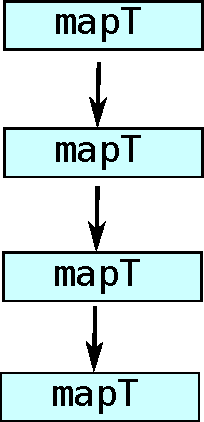
\includegraphics[width=1.6cm]{img/BlackScholes-unfused.pdf} &
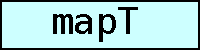
\includegraphics[width=1.6cm]{img/BlackScholes-fused.pdf} &
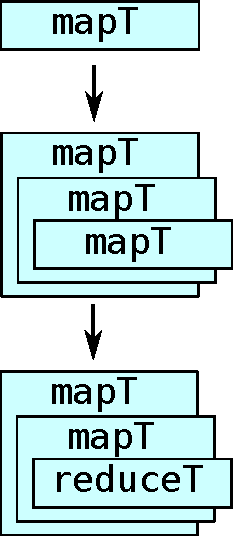
\includegraphics[width=1.6cm]{img/MatMultFun-unfused.pdf} &
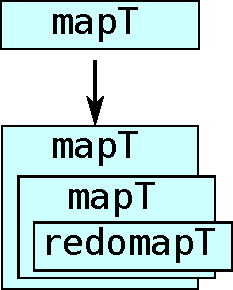
\includegraphics[width=1.6cm]{img/MatMultFun-fused.pdf} &
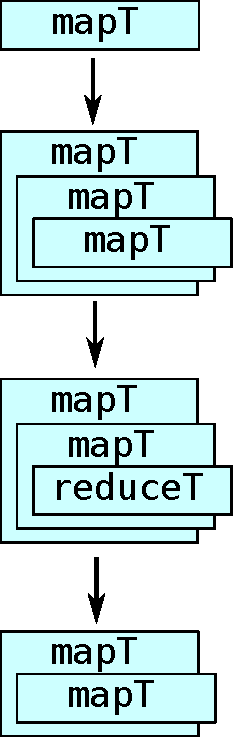
\includegraphics[width=1.6cm]{img/BabyBear-unfused.pdf} &
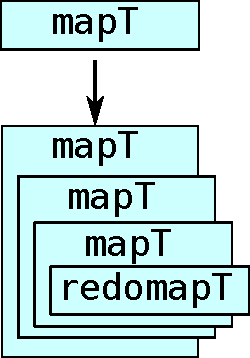
\includegraphics[width=1.6cm]{img/BabyBear-fused.pdf}
\end{tabular}
\caption{Artificial benchmark dataflows, before and after optimisation}
\label{fig:artificial-dataflows}
\end{figure}

The structure of the artificial benchmarks are shown on
\cref{fig:artificial-dataflows}.  P0, being a straightforward sequence
of four \texttt{map}s, fuses well.  P1 also fuses well - the main loop
becomes a two-dimensional \texttt{tmap}, with the dot product at each
location being computed in a \texttt{redomap}.  Although not visible
in the data flow diagram, it is worth remarking that hoisting has
moved all \texttt{assert} expressions (originating in the use of
\texttt{zip}) out of the main loop, which can thus be evaluated with
no bounds checking - or indeed, any branching at all.

There is clearly a missed opportunity for fusion, though, the reason
for which becomes clear when we inspect the code around the unfused
\texttt{map}:
\begin{colorcode}
...
let {untuple_13} =
  mapT(fn \{[[int]]\} ([int] param_0_8) =>
         // tmp_repl_11 aliases param_0_8
         let tmp_repl_11 = replicate(N_2, param_0_8) in
         \{tmp_repl_11\},
       x_0) in
let tmp_size_14 = size(2, untuple_13) in
... // untuple_13 is eventually input to main loop.
\end{colorcode}
The size analyser is not smart enough to rewrite the \texttt{size}
expression, and \texttt{untuple\_13} is thus used several times,
blocking fusion.  The most reasonable solution is to improve the size
analyser, for which a potential approach is outlined in
\cref{sec:future-work}.  P2 suffers from the same problem, although
again the main loop is fully fused.

When illustrating the dataflow for the real-world benchmarks, I
performed some minor simplifications.  Specifically, prologue and
epilogue code has been removed in order to emphasise the main loop.

\begin{figure}
\begin{center}
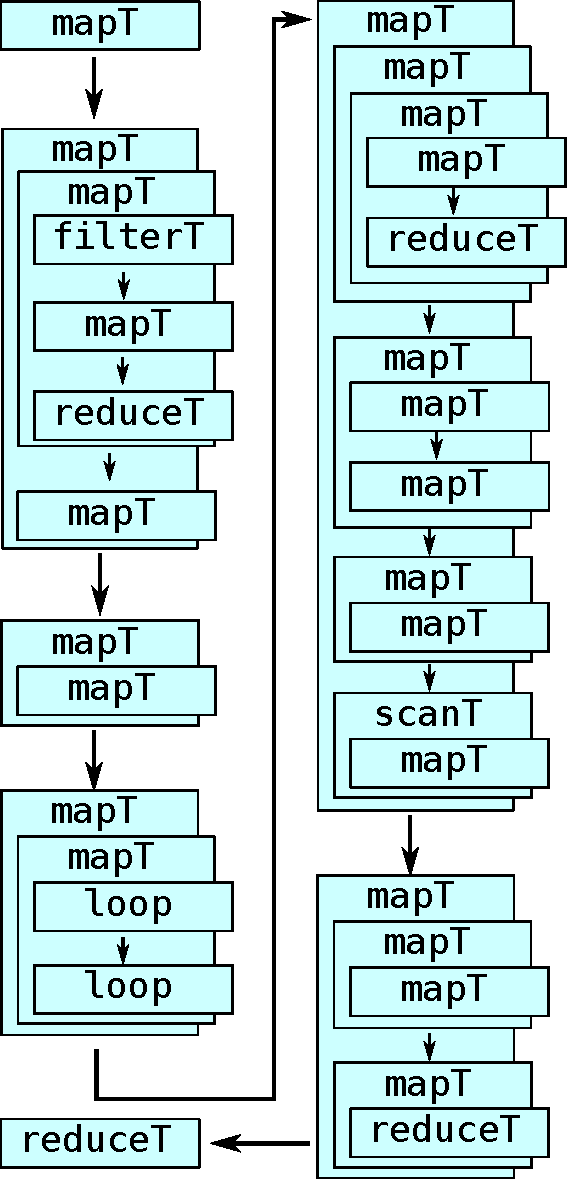
\includegraphics[width=3.2cm]{img/PricingLexiFi-unfused.pdf}
\hspace{1cm}
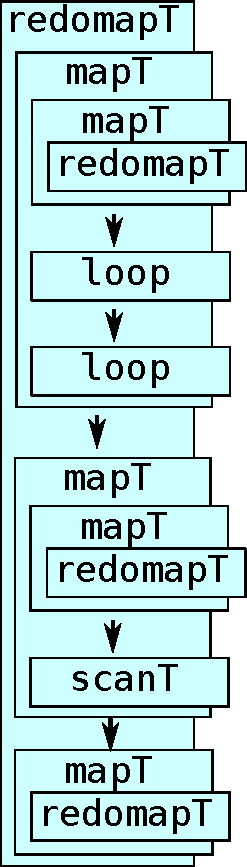
\includegraphics[width=1.6cm]{img/PricingLexiFi-fused.pdf}
\end{center}
\caption{R0 benchmark dataflow, before and after optimisation}
\label{fig:r0-dataflow}
\end{figure}

Of the real-world benchmarks, R0, whose dataflow is illustrated on
\cref{fig:r0-dataflow}, benefits the most from optimisations.  The
program is turned into a big \texttt{redomapT} that runs over an array
of a thousand elements.  The body of the \texttt{redomapT} runs three
loops in sequence.  The two first could in principle be fused, but we
are again foiled by limitations of the size analyser.  In this case,
the use of an explicit \texttt{loop} prevents the size analyser from
determining the column size of the two-dimensional array returned by
the \texttt{mapT}.  The fusion of R0 also requires fusing across
\texttt{transpose} and \texttt{reshape}.

\begin{figure}
\begin{center}
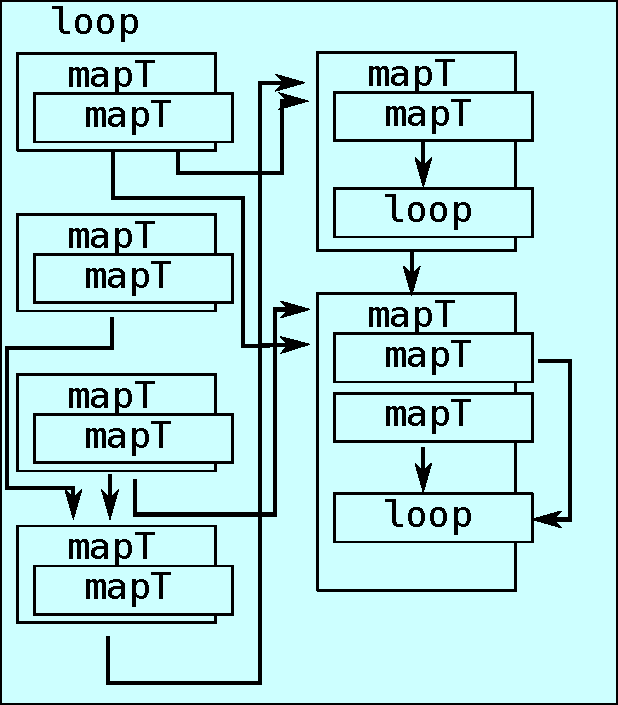
\includegraphics[width=3.2cm]{img/HiperfitEgCos-unfused.pdf}
\hspace{1cm}
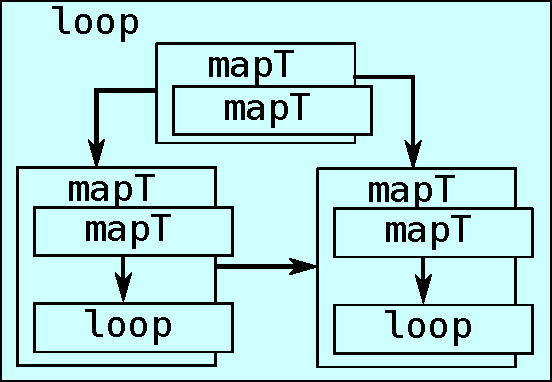
\includegraphics[width=3.2cm]{img/HiperfitEgCos-fused.pdf}
\end{center}
\caption{R1 benchmark dataflow, before and after optimisation}
\label{fig:r1-dataflow}
\end{figure}

For R1, the gains are more muted.  The overall structure is a
sequential, iterative main loop, which of course limits what we can
do, but the body of this loop can in principle be parallelised.  The
unoptimised and optimised loop bodies can be seen on
\cref{fig:r1-dataflow}.  At first sight, two possible avenues for
further fusion are possible:

\begin{enumerate}
\item The first \texttt{mapT} could be fused into its two consumers.
  While this would surely duplicate computation, perhaps it is
  worthwhile in this case.  Inspecting the code, which is shown in
  \cref{fig:r1-unfused-map}, we find that the computation that would
  be duplicated for each element is approximately four primitive
  arithmetic operations, and two calls to exponent and logarithm
  functions.  Such duplication would likely be acceptable in this
  case, as it enables an instance of fusion.

\item The reason for why the two latter \texttt{mapT}s are not fused
  is more tricky.  Although not expressed in the diagram, the input to
  the rightmost \texttt{mapT} is \textit{transposed}, and we have no
  fusion rule capable of handling a transposition in this case, as
  neither consumer nor producer is a map nest.

  It is not immediately clear how this could be solved.
\end{enumerate}

\begin{figure}
\begin{center}
\begin{bcolorcode}
mapT(fn \{*[real], *[real], *[real], *[real]\} (real xi_481) =>
       let tmp_call_488 = log(xi_481) in
       let bop_493 = 0.5 * tmp_call_488 in
       let \{soac_v_506, soac_v_507, soac_v_508, soac_v_509\} =
         mapT(fn \{real, real, real, real\} (real yj_495) =>
                let bop_496 = bop_493 + yj_495 in
                let bop_498 = bop_496 - bop_477 in
                let val_504 = 2.0 * bop_498 in
                let tmp_call_505 = exp(val_504) in
                \{0.0, tmp_call_505, 0.0, 0.36\},
              untuple_247) in
       \{soac_v_506, soac_v_507, soac_v_508, soac_v_509\},
     untuple_130)
\end{bcolorcode}
\end{center}
\caption{Unfused map in R1}
\label{fig:r1-unfused-map}
\end{figure}

\begin{figure}
\begin{center}
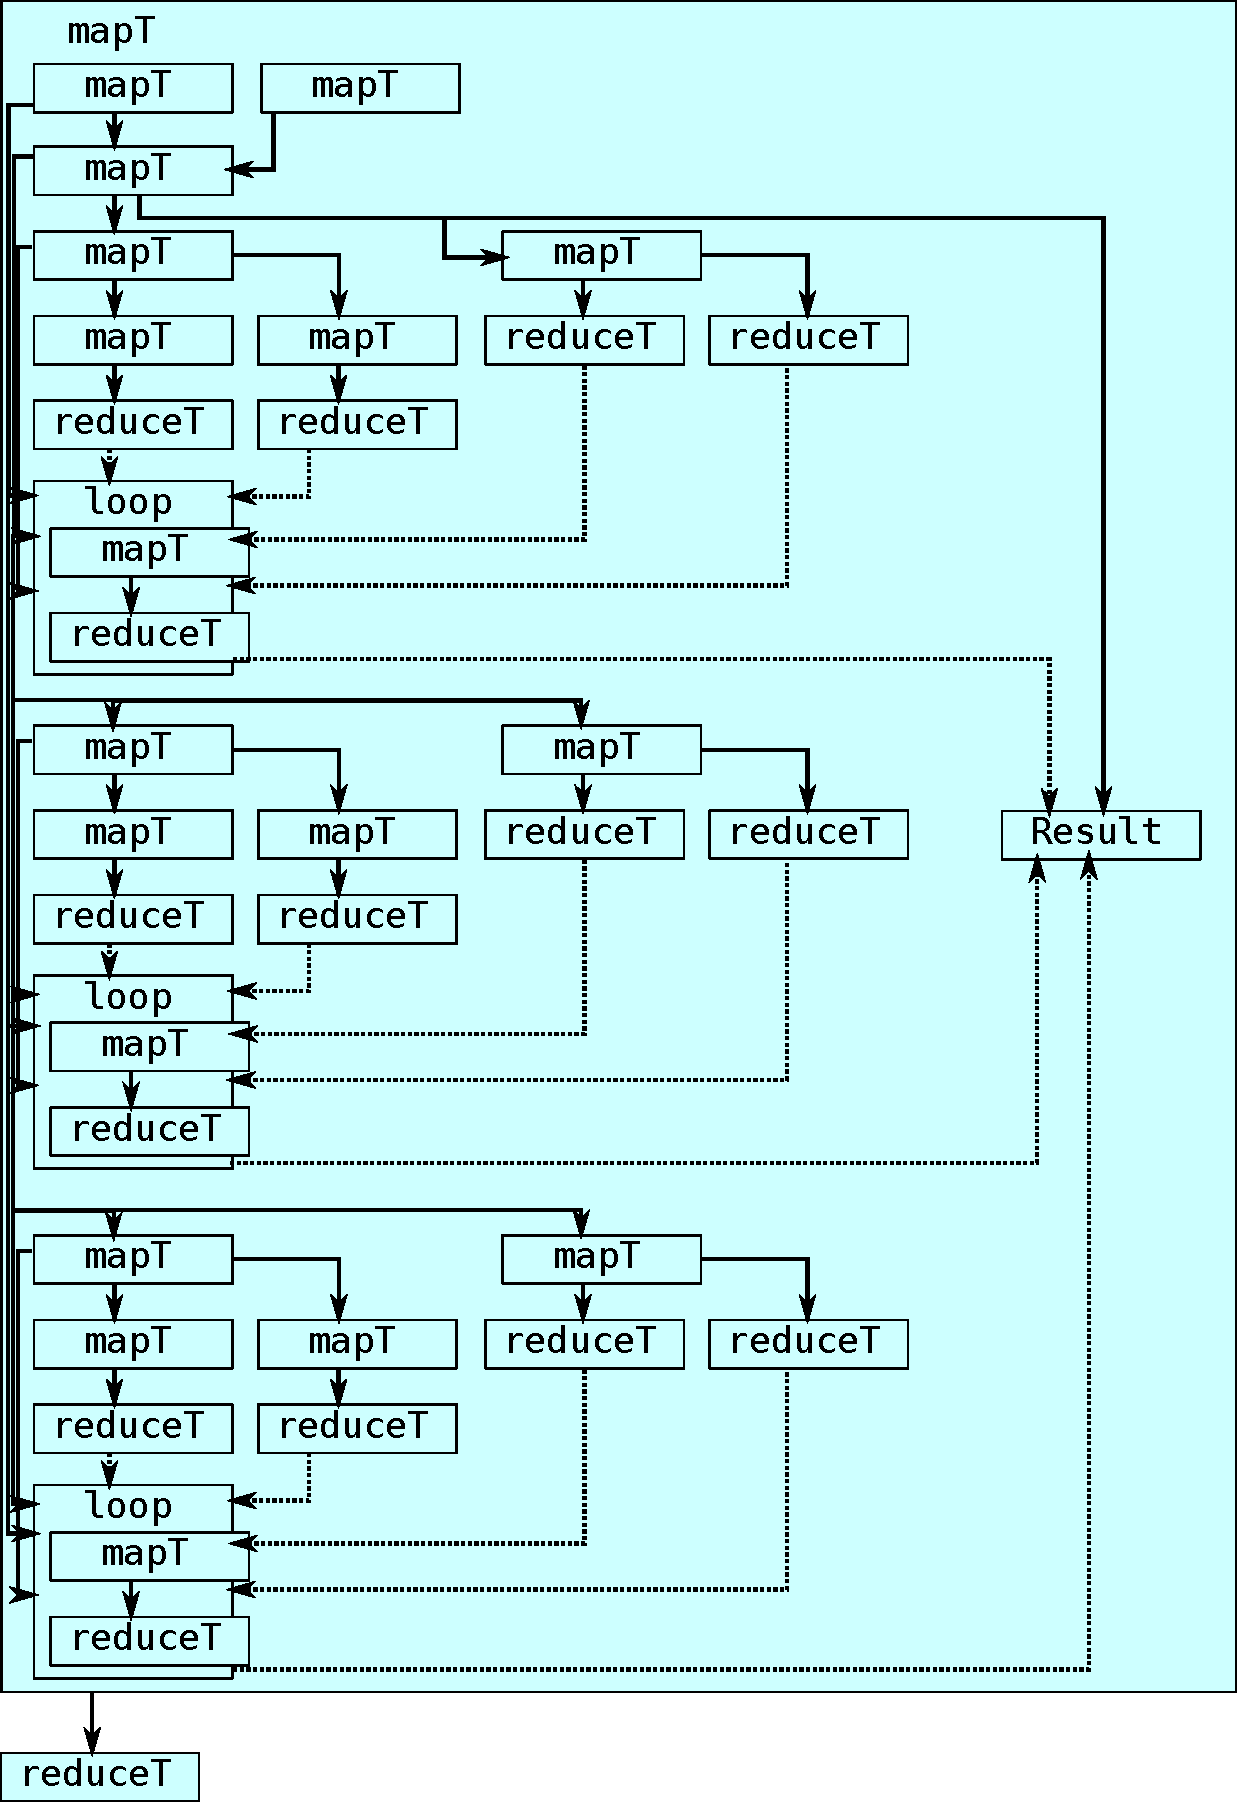
\includegraphics[width=5.7cm,valign=t]{img/CalibLexiFi-unfused.pdf}
\hspace{0.2cm}
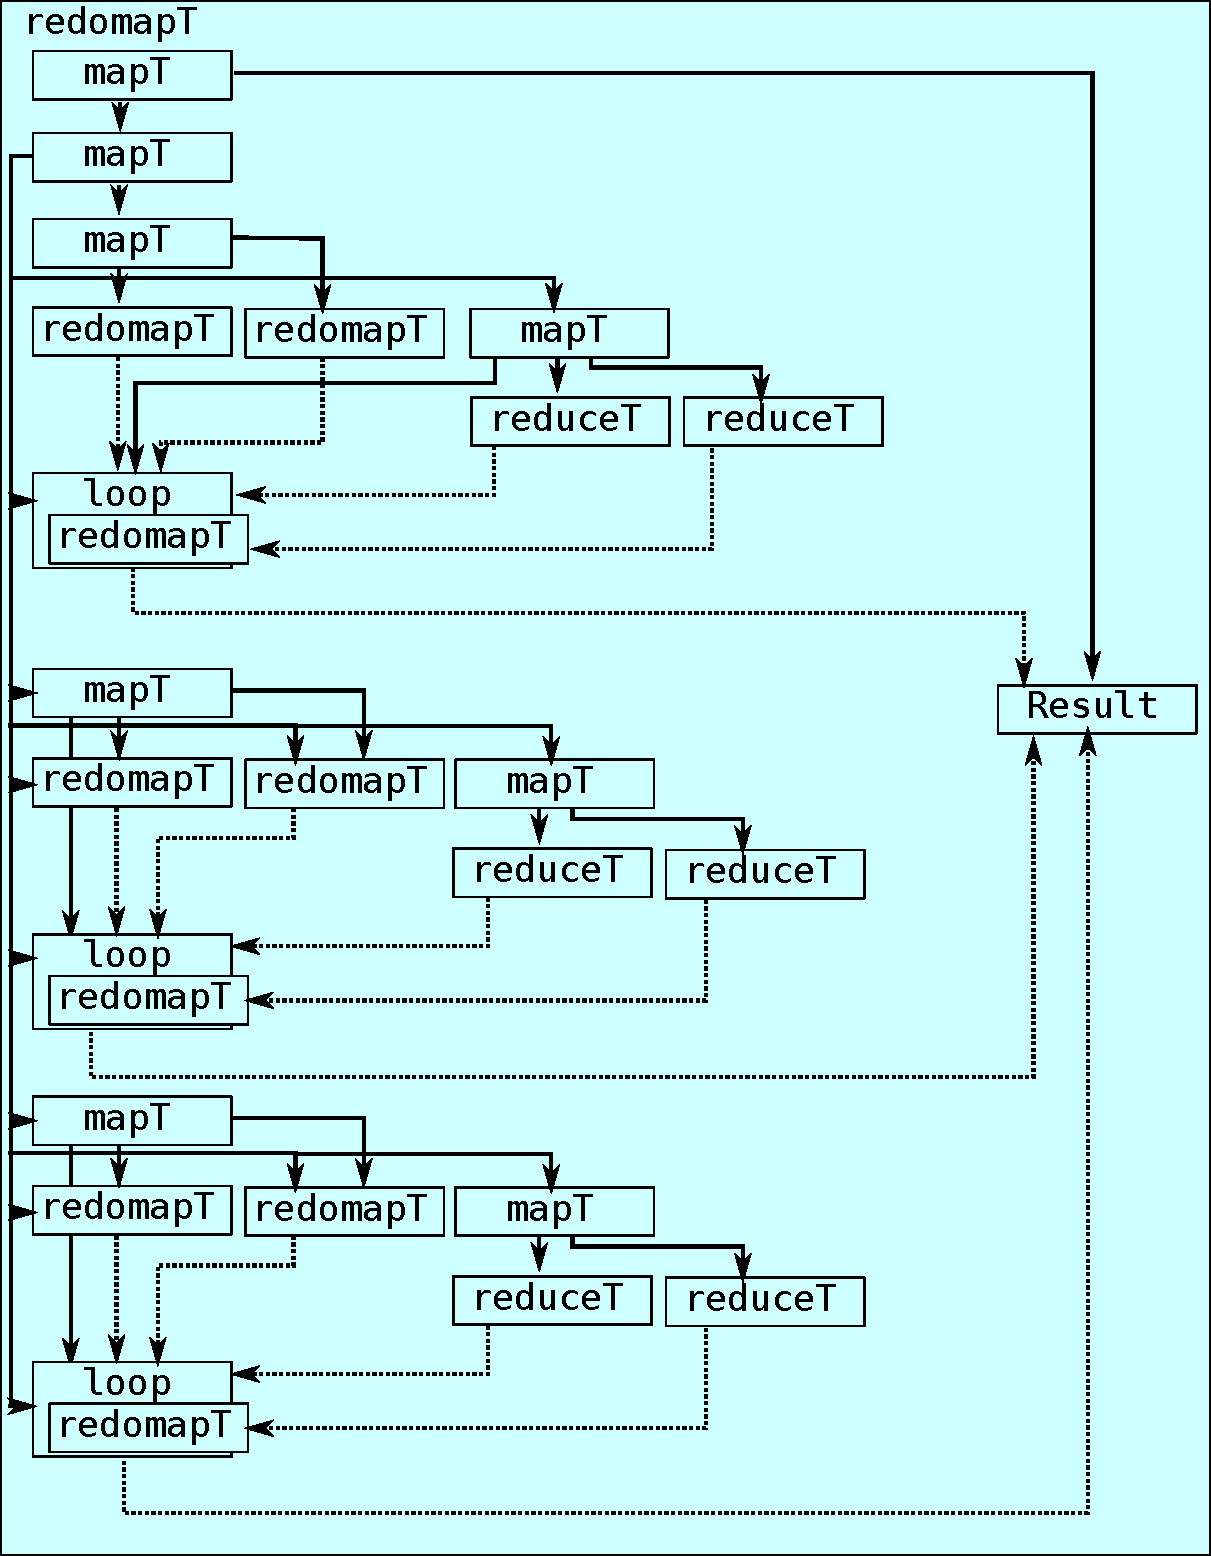
\includegraphics[width=5.7cm,valign=t]{img/CalibLexiFi-fused.pdf}
\end{center}
\caption{R0 benchmark dataflow, before and after optimisation}
\label{fig:r2-dataflow}
\end{figure}

R2 is easily the most complex benchmark, and also the one for which
fusion has the smallest impact on the data flow graph.  As shown on
\cref{fig:r2-dataflow}, the body of the main loop contains three
independent (but near-identical) loops whose results are combined
using a non-fusible series of reductions (summarised as a single
node).  The optimised structure is virtually identical: the only
optimisation is a few instances of \texttt{map}-\texttt{map} and
\texttt{map}-\texttt{reduce} fusion.  However, it is worth noting that
there are instances where we take advantage of our fusion algorithms
ability to fuse just part of the input to a SOAC.

\begin{figure}
\begin{center}
\begin{bcolorcode}
...
let \{soac_v_685, soac_v_686\} =
  mapT(fn \{real, real\} (real arg_675, real arg_676, real arg_677, real arg_678) =>
         let baix_679 = arg_675 * mux_239 in
         \{arg_677 * exp(-baix_679),
           (arg_678 - baix_679) / arg_676\},
       soac_v_669, soac_v_670, soac_v_671, soac_v_672) in
let \{untuple_690\} =
  reduceT(fn \{real\} (real x_687, real y_688) =>
            \{x_687 + y_688\},
          \{0.0\}, soac_v_685) in
let \{untuple_695\} =
  reduceT(fn \{real\} (real param_0_691, real param_1_692) =>
            if param_0_691 < param_1_692
            then \{param_1_692\}
            else \{param_0_691\},
          \{-10000000000000000000000000000000000000000000000000.0\},
          soac_v_686) in
...
\end{bcolorcode}
\end{center}
\caption{Unfused loops in R2}
\label{fig:r2-unfused-loops}
\end{figure}

As in R1, each of the three inner loops have a case where multiple
uses of the output of a \texttt{mapT} SOAC prevents us from fusing it
into a \texttt{reduceT}.  Again, it is worth inspecting the code to
see whether our reluctance to duplicate computation is again too
conservative.  The code in question (slightly simplified for
readability) is shown on \cref{fig:r2-unfused-loops}.

Again we see that that a relatively cheap \texttt{mapT} operation
cannot be fused without duplicating computation.  This case is
particularly interesting, because the \texttt{mapT} conceptually
computes two distinct arrays, with only the computation of
\texttt{baix\_679} (a single multiplication per element) being shared.
This structure was also present in the original program.  In a future
elaboration of the fusion algorithm, it may be worthwhile to split
SOACs apart to make the representation of shared computation even more
precise.

\section{Runtime results}
\label{sec:runtime-results}

The real-world benchmarks were repeatedly passed through \LO{}
optimisations until no further transformation was achieved, then
compiled with a code generator generating sequential C code.

The resulting programs were compiled with GCC 4.8.2 using maximum
optimisation (\texttt{-O3}) on an Intel Core i7-2630QM CPU running at
2.00GHz.  Each program was executed one thousand times and the
run-times averaged.  The results are shown on \cref{fig:speedups}

\begin{figure}
\begin{center}
\begin{tabular}{l|c|c|c}
   & \textbf{Unoptimised} & \textbf{Fused} & \textbf{Speedup} \\\hline
R0 & 0.430s & 0.292s & 46\% \\
R1 & 0.098s & 0.057s & 71\% \\
R2 & 0.061s & 0.047s & 31\%
\end{tabular}
\end{center}

\caption{Benchmark runtimes}

\label{fig:speedups}
\end{figure}

It is hard to determine how much of the speedup is due to fusion in
isolation and how much is due to other optimisations, as they all
interact to enable each other.  However, given that the C programs
were compiled with full optimisation, it is likely that the C compiler
performed much hoisting and most of our simpler optimisations itself.

%%% Local Variables: 
%%% mode: latex
%%% TeX-master: "thesis.tex"
%%% End: 


\chapter{Conclusions}
\label{chap:conclusions}

This chapter summarises the result of our work.
\Cref{sec:related-work} compares our fusion algorithm with fusion in
other data-parallel programming languages, as well as looking at other
approaches to uniqueness typing.  \Cref{sec:future-work} outlines a
number of possible future improvements to \LO{} and the compiler.
\Cref{sec:conclusion} provides a final summary of the results of this
thesis.

\section{Related Work}
\label{sec:related-work}

Our approach to performining fusion, via rewrite rules, is not unique
by itself, as this is the approach used in e.g. Data-Parallel
Haskell~\cite{Chak06DPH} (DPH).  What sets us apart is the fact that
our rewriting rules are defined on the dataflow graph, and not the
program itself.  While DPH obtains good results, its rewrite rules are
quite limited -- they are an inherently local view of the program, and
would be unable to cope with limitations in the presence of in-place
array updates, and whether the result of an array operation is used
multiple times.  The Glasgow Haskell Compiler itself also bases its
list fusion on rewrite rules and cross-module
inlining~\cite{jones2001playing,gill1993short}.

The Repa~\cite{keller2010regular} approach to fusion is based on a
delayed representation of arrays, which models an array as a function
from index to value.  With this representation, fusion happens
automatically through function composition, although this can cause
duplication of work in many cases.  To counteract this, Repa lets the
user \textit{force} an array, by which it is converted from the
delayed representation to a traditional sequence of values.  The pull
arrays of Obsidian~\cite{claessen2012expressive} use a similar
mechanism.  This approach puts the onus on the programmer to specify
points where the manifestation of arrays is beneficial, even though
this may be a low-level consideration that depends on details of the
target hardware.  We therefore consider this a job better suited for
the compiler.

Accelerate~\cite{mcdonell2013optimising} uses an elaboration of the
delayed arrays representation from Repa, and in particular manages to
avoid duplicating work.  All array operations have a uniform
representation as constructors for delayed arrays, on which fusion is
performed by tree contraction.  Accelerate supports multiple arrays as
input to the same array operation (using a \texttt{zipWith}
construct).  Although arrays are usually used at least twice (once for
getting the size, once for the data), it does not seem that they can
handle the difficult case where the output of an array operation is
used as input to two other array operations.

NESL has been extended with a GPU backend~\cite{bergstrom2012nested},
for which the authors note that fusion is critical to the performance
of the flattened program.  The NESL approach is to use a form of
copy-propagation on the intermediary code, and lift the resulting
functions to work on entire arrays.  This approach only works for what
we would term \texttt{map}-\texttt{map} fusion, however.

Our uniqueness attributes have some similarities to the ``owning
pointers'' found in the impure language Rust~\cite{rust}, albeit there
are deep differences.  In Rust, owning pointers are used to manage
memory -- when an owning pointer goes out of scope, the memory it
points to is deallocated -- while we use uniqueness attributes to
handle side effects.  In addition, we allow function calls to consume
arrays passed as unique-type parameters, whereas in Rust this causes a
deep copy of the object referenced by the owning pointer.

A closer similarity is found in the pure functional language Clean,
which contains a sophisticated system of uniqueness
typing~\cite{barendsen1996uniqueness}.  Clean employs uniqueness
typing to re-use memory in cases where a function receives a unique
argument, but also (and perhaps more importantly) to control side
effects including arbitrary I/O.  As in \LO{}, alias analysis is used
to ensure that uniqueness properties are not violated.  A notable
difference is that the Clean language itself does not have any
facilities for consuming unique objects, apart from specifying a
function parameter as unique, but delegate this to (unsafe) internal
functions, that are exposed safely via the type system.  Furthermore,
a unique return value in Clean may alias some of the parameters to the
function, which is forbidden in \LO{}.  We have found that this
greatly simplifies analysis, and allows it to be fully
intraprocedural.

\section{Future Work}
\label{sec:future-work}

A very important immediate goal is the implementation of a code
generator targeting GPU execution.  Furthermore, a number of other
avenues for further research and development of \LO{} ae available.

\subsection{Size Information in Type System}

The size analysis presented in \cref{chap:hindrance-removal} is quite
restricted, and was designed and extended on an ad-hoc basis in order
to enable fusion of the real-world benchmarks.  Considering the great
importance of accurate size information in not only doing high-level
optimisations, but also generating efficient low-level code, it
appears very worthwhile to integrate tracking of array sizes into the
language itself.

We suggest a type system extension inspired by \textit{dependent
  types}, although much simpler.  As an example, let us look at how we
would like to be able to define matrix multiplication:

\begin{colorcode}
fun [[int,N],P] matMult([[int,N],M] a, [[int,M],P] b ) =
  ...
\end{colorcode}

This function declares that it takes two \texttt{int} array arguments,
the first of size $N \times M$ and the second of size $M \times P$,
and returns an integer array of size $N \times P$.  Any caller of
\texttt{matMult} must first prove to the type system that the
arguments have the correct size, while \texttt{matMult} itself must
prove that its body always returns an array of the appropriate size.

Such a proof could be provided through a mechanism much like the
current \texttt{assert}, which allows us a sort of ``escape hatch''
for when we cannot statically guarantee the size of our data - for
example, when it is given to us as input from the outside world, or
the result of a \texttt{filter}.  As the current \LO{} compiler is
already able to optimise and hoist many assertions away, this would be
useful by itself.

However, this would not solve the problem encountered in
\cref{chap:optimisation-results}, when the inability to transform a
\texttt{size} expression prevented fusion in program R0.  The
problematic part of R0 has this essential structure (where \texttt{N}
is some variable in scope):

\begin{colorcode}
let b = map(fn [real] (int x) =>
              let xa = replicate(N,x) in
              loop (xa) = for i < N do
                let xa = f(xa) // Does not change size of xa
                in
              xa,
            a) in
let n = size(1,b) in
map(g(n), b)
\end{colorcode}

The current ad-hoc size analyser is not smart enough to figure out the
inner size (\texttt{N}) of the array \texttt{b}.  Integrating size
information into the type system would allow us to annotate the return
type of the anonymous function as follows:

\begin{colorcode}
let b = map(fn [real,\emp{N}] (int x) =>
              ...,
            a) in
...
\end{colorcode}

We now statically promise that the inner size of \texttt{b} will
always be \texttt{N}, possibly backed by an assertion within the body
of the map.  The intent is that this promise can be checked by the
type-checker.  Presumably, for the body of the function to be
type-correct, the function \texttt{f} would have been defined to
return an array of the same size as its input.

It is not yet clear exactly how we should deal with cases where the
size of an array dimension cannot be statically known, or where it is
the result of a complex expression.  It is not desirable to support
the full power of dependent types, nor to include a full theorem
prover in \LO{}, as this could make it very cumbersome to use \LO{} as
a compiler target language.  In the end, it is important to remember
that our primary motivation is to improve size tracking for the
benefit of optimisation and code generation.

\subsection{Improved Aliasing Analysis}
\label{sec:improved-aliasing-analysis}

The system of uniqueness types presented in
\cref{chap:uniqueness-types} hinges crucially on tracking potential
sharing between arrays.  However, the current model of aliasing is
very coarse-grained, as it cannot describe sharing at a more precise
level than entire arrays.  For example, assume that we have the
following function:

\begin{colorcode}
  fun *[int] replace(*[int] arr, int i, int x) =
    let arr[i] = x in arr
\end{colorcode}

The result of \texttt{replace(a,i,x)} is the array \texttt{a} with the
element at index \texttt{i} replaced by \texttt{x}.  We may want to
use this function to replace an element within a slice of an array,
like so\footnote{Of course, in this contrived example, we could just
  use \texttt{let-with} rather than a separate function.}:

\begin{colorcode}
let b = a with [j] <- replace(a[j], j, x) in
...
\end{colorcode}

Unfortunately, this code will be refused by the compiler: The call to
\texttt{replace} consumes the array \texttt{a}, because \texttt{a[j]}
is aliased with \texttt{a}, yet \texttt{a} is used as the source in a
let-binding.  Making a separate binding for the call to
\texttt{replace} may make things more clear:

\begin{colorcode}
let r = replace(a[j], j, x) in \emp{// Consumes a}
let b = a with [j] <- r in
...
\end{colorcode}

As far as the type system is concerned, both the call to
\texttt{replace} and the \texttt{let-with} expression consume the
entirety of \texttt{a}, hence causing a compile-time
double-consumption error.  The only solution is to use \texttt{copy}:

\begin{colorcode}
let r = replace(\emphh{copy}(a[j]), j, x) in \emp{// Consumes a}
let b = a with [j] <- r in
...
\end{colorcode}

It is clear to us however, that the call to \texttt{replace} only
modifies the memory associated with the \texttt{j}th row of
\texttt{a}.  Furthermore, when \texttt{a} is next accessed (and
consumed), the \texttt{j}th row is replaced anyway.  Thus, it should
be possible to perform this entire operation in $O(1)$ space.

We could of course make a specialised variant of \texttt{replace} for
two-dimensional arrays, but this leads to unnecessary code bloat.
Thus, we believe that more precising tracking of sharing would be
worthwhile.  The problem is not easy, however, as the expression for
the array index may be arbitrarily complicated.

\subsection{Array Views}

Array indexing in \LO{} is quite limited - only entire dimensions can
be extracted.  With \texttt{split}, we can get slightly more control,
but extracting e.g. the inner elements of a $2$-dimensional array is
an enormously clumsy affair, as illustrated on
\cref{fig:inner-elements-l0}.

\begin{figure}
\centering
\begin{subfigure}[t]{.5\textwidth}
\begin{colorcode}
fun [[int]] inner([[int]] a) =
  let n = size(0,a) in
  let m = size(1,a) in
  let \{_,a2\}   = split(1,a) in
  let \{rows,_\} = split(n-2,a2) in
  map(fn [int] ([int] row) =>
        let \{_, row2\} =
          split(1,row) in
        let \{res, _\}  =
          split(m-2,row2) in
        res,
      rows)
\end{colorcode}
\subcaption{\LO{} \label{fig:inner-elements-l0}}
\end{subfigure}\hfill
\begin{subfigure}[t]{.4\textwidth}
\begin{colorcode}
def inner(a):
  a[1:-1, 1:-1]










\end{colorcode}
\subcaption{Numpy \label{fig:inner-elements-numpy}}
\end{subfigure}
\caption{Removing the outer elements of a $2$-dimensional array}
\label{fig:inner-elements}
\end{figure}

The primary reason for this is that \texttt{split} only slices the
outer dimension.  In other systems, such as the Python library
Numpy~\cite{oliphant2006guide}, it is comparatively much simpler to
simultaneously slice on every dimension of an array, as illustrated on
\cref{fig:inner-elements-numpy}.

As an array-oriented programming language, \LO{} should have similar
convenient support for slicing arrays.  It is not only practical when
writing code, but the resulting slice expressions are much easier to
analyse than a dense expression using \texttt{size} and
\texttt{split}.

More radically, many operations in \LO{} are operationally just
transformations of the index space of an underlying array.
Transpositions, \texttt{reshape}, \texttt{replicate}, and even array
indexing, merely provide different views of underlying data.  Thus,
perhaps the best solution would be to provide a language construct
that can express this mapping directly.  We can envision a syntax like
the following:

\begin{colorcode}
fun [[int]] transpose([[int]] a) =
  \emphh{arrange} a as
    size (n,m) => (m,n) \emp{// Determine size of output array}
    elem [i,j] => [j,i] \emp{// Map position (i,j) in output to position (j,i) in input}
\end{colorcode}

A crucial property is that every element of the output array maps
directly to some element in the input array, which means that at
compile time, we can remove the \texttt{arrange} intermediary and
access the original array directly.  This design is very similar to
the delayed arrays of Repa~\cite{keller2010regular}, which represent
arrays as a function from the index space to the value space.  The
built-in \texttt{replicate} could be reformulated as follows:

\begin{colorcode}
fun [[[int]]] replicate(int k, [[int]] r) =
  \emphh{arrange} r as
    size (n,m)   => (k,n,m)
    elem [i,j,p] => [j,p]
\end{colorcode}

We can also express entirely novel transformations, such as a
rearrangement that repeats every element of its input array twice:

\begin{colorcode}
fun [int] dupElem([int] a) =
  \emphh{arrange} a as
    size (n)     => (n)
    elem (2*i)   => [i]
    elem (2*i+1) => [i]
\end{colorcode}

A large potential problem with a construct such as \texttt{arrange} is
whether the compiler will be able to recognise ``known''
transformations.  For example, we demonstrated in
\cref{chap:fusion-enabling-soac-transformations} that the fusion
algorithm depends on being able to recognise and rewrite
\texttt{transpose} expressions, which it must be able to do, even if
they are formulated in terms of \texttt{arrange}.  Hence, it would be
important that every \texttt{arrange} can be reduced to a canonical
form that uniquely represents the transformation it performs.

\subsection{Software Engineering}

The world already has plenty of papers and theses stuffed with long
listings of Haskell code, and we have therefore tried to shy away from
talking too much about the software architecture of the \LO{}
compiler.  While the overall code base is healthy and well-structured,
there are still several instances of technical debt that should be
paid off:

\begin{itemize}
\item While the compiler is nicely divided into discrete passes, the
  order in which said passes should be invoked is a bit unclear.  As
  it stands, programs are passed through every pass several times,
  simply to ensure that they get optimised fully.  This requires some
  bit of re-engineering, probably also involving changing some passes
  (particularly the fusion module) to be less sensitive as to the
  shape of the input program.

\item For this thesis, \LO{} has been divided into an external and
  internal language.  In the compiler, both of these are included in
  the same abstract syntax tree definition, with most passes either
  silently ignoring or loudly crashing if they encounter a construct
  that belongs to the external language.  This creates undue
  complexity, and should be resolved by splitting the language more
  clearly, even if the cost is some code duplication (for example, we
  might need separate but very similar parsers).

\item Somewhat related to the previous issue, the \LO{} syntax tree
  definition does not statically enforce normalisation.  Again,
  compiler passes either ignore them or crash when an un-normalised
  term is encountered.

\item Many optimisations depend on every variable in the program
  posessing a unique name.  This property is ensured by tagging each
  input name with a unique integer, then passing around a counter that
  can be used to generate fresh, globally unique integers.
  Unfortunately, many transformations (e.g. inlining) end up
  duplicating bits of code, which then have to be entirely renamed in
  order to preserve uniqueness.  Furthermore, passing the counter
  around is cumbersome, even if packaged in a state monad.  An
  alternative approach to handling name binding, based on de Bruijn
  indices~\cite{McBride:2004:FPI:1017472.1017477}, is being
  considered.  Such an approach would allow us to get rid of the
  counter, while still being able to cheaply avoid unwanted name
  capture.
\end{itemize}

\section{Conclusion}
\label{sec:conclusion}

In this master’s thesis, we have presented the design of a pure
functional data-parallel language, with a design that enables both (i)
a degree low-level imperative programming, as well as (ii) supporting
high-level structural transformations such as loop fusion.  The
language contains a type system for in-place modification and aliasing
of arrays and array slices that ensures referential transparency,
which in turn supports equational reasoning.

Previous work on fusion has taken two main directions: Either fusion
is performed aggressively, and the programmer is provided primitives
to inhibit fusion, for example by forcing array to materialise, or
fusion is performed via rewriting rules on the syntax tree.  The
latter approach relies tightly on the inliner engine, and its
applicability is limited to the case when each fused array is consumed
by one array combinator.

This thesis has presented a program-level, structural-analysis
approach to fusion that handles the difficult case in which an array
produced by a second-order array combinator (SOAC), such as
\texttt{map}, is consumed by several other SOACs (if the SOAC
producer-consumer dependency graph is reducible).  This essentially
allows fusion to operates across \texttt{zip}/\texttt{unzip}.

Furthermore, we have shown a compositional algebra for fusion that
includes array combinators, such as \texttt{map}, \texttt{reduce},
\texttt{filter}, \texttt{scan}, and \texttt{redomap}, and other
built-in functions that would otherwise hinder fusion applicability,
such as \texttt{size}, \texttt{transpose}, and \texttt{reshape}.  This
algebra also includes transformations that in come cases allow fusion
with \texttt{scan} as both consumer and producer.

%%% Local Variables: 
%%% mode: latex
%%% TeX-master: "thesis.tex"
%%% End: 


\clearpage

\part{Closing Credits}

% We want the bibliography in the ToC, but it shouldn't have a chapter
% number.
\phantomsection
\addcontentsline{toc}{chapter}{Bibliography}
\defbibheading{bibliography}{\chapter*{Bibliography}}
\printbibliography

\backmatter
\appendix
\chapter{Artificial Benchmark Programs}
\label{app:artificial-benchmark-programs}

\section{P0}

\verbatiminput{../benchmarks/BlackScholes.l0}

\section{P0 -- optimised}

\verbatiminput{../benchmarks/BlackScholes-fused.l0}

\section{P1}

\verbatiminput{../benchmarks/MatMultFun.l0}

\section{P1 -- optimised}

\verbatiminput{../benchmarks/MatMultFun-fused.l0}

\section{P2}

\verbatiminput{../benchmarks/BabyBearFun.l0}

\section{P2 -- optimised}

\verbatiminput{../benchmarks/BabyBearFun-fused.l0}

%%% Local Variables:
%%% mode: latex
%%% TeX-master: "thesis"
%%% End:


\end{document}
